% =====================================================================
%  Manuscript for Pharmaceutical Statistics (portable Overleaf version)
%  Regenerated from docs/manuscript_full_draft_pharm_stats.md
%  (source of record). Numbers are the genuine two-head DeepSets
%  evidence package; keep this .tex in sync with the .md.
%
%  This uses the standard `article` class so it compiles on Overleaf
%  with no extra .cls upload. For the official Wiley submission format,
%  replace the class line with the Wiley NJD template, e.g.
%     \documentclass[AMA,STIX1COL]{WileyNJD-v2}
%  (upload WileyNJD-v2.cls + WileyNJD-AMA.bst from the Wiley
%  "Pharmaceutical Statistics" author template), then the body below
%  should transfer with minimal changes.
% =====================================================================
\documentclass[11pt]{article}

\usepackage[T1]{fontenc}
\usepackage[utf8]{inputenc}
\usepackage{lmodern}
\usepackage[margin=1in]{geometry}
\usepackage{amsmath,amssymb}
\usepackage{booktabs}
\usepackage{longtable}
\usepackage{array}
\usepackage{graphicx}
% Figure files live in results/figures/final_v2/ (vector PDF + 300 dpi TIFF).
% On Overleaf, upload those PDFs (flat) — the first path below then applies.
\graphicspath{{figures/}{../results/figures/final_v2/}{results/figures/final_v2/}}
\usepackage{xcolor}
\usepackage[hidelinks]{hyperref}
\usepackage{enumitem}
\usepackage{setspace}
\usepackage{float}
% Lightweight algorithm float (portable; no algorithmicx/algorithm2e needed).
\floatstyle{ruled}
\newfloat{algorithm}{htbp}{loa}
\floatname{algorithm}{Algorithm}

\newcommand{\lamz}{\lambda_{0}}
\setlength{\parskip}{0.4em}
\setlength{\parindent}{0pt}

\title{Retrospective predictive calibration of oncology trial similarity
for Bayesian historical borrowing}

\author{[Author names and affiliations to be completed by the authors]}
\date{\today}

\begin{document}
\maketitle

% ---------------------------------------------------------------------
\begin{abstract}
\noindent\textbf{Background.} Bayesian historical borrowing can sharpen the
estimate of an objective response rate (ORR) in a small oncology trial, but
its value depends on \emph{which} historical evidence is used and on the
frame in which its error rates are assessed. Textual similarity between
registry records is not sufficient for the first, and --- since strict
worst-case type~I control forfeits the power gains of borrowing in
one-parameter designs of the kind studied here ---
nominal safety language is not sufficient for the second.

\noindent\textbf{Methods.} An explainable retrieve--rerank--borrow pipeline
converts ClinicalTrials.gov records into a beta-binomial mixture prior via
a \emph{selective} two-head DeepSets model (per-candidate mixture weight
and information discount; set-level total borrowing), anchored at an
intercept-only empirical-Bayes (EB) prior that is also the reference for
every comparison. The \emph{final design} adds a historical mixture-mass
cap of $0.5$ and contains no outcome-adaptive component (SAM retained as
sensitivity only). Evaluation separates a \emph{primary analysis} ---
donor availability enforced at decision time, on an audit-informed
title-screened binary-response subset of measured $\approx 80\%$ purity --- from a
hypothetical full-information upper bound, and assesses simulation
operating characteristics under a worst-case frame and an exploratory
corpus-specific decision analysis (mixing measure = the corpus-estimated
drift distribution; tolerated pointwise inflation ceiling $0.05$;
thresholds fixed on one batch, re-evaluated on an independent
five-fold-larger batch; between-design comparisons size-adjusted).

\noindent\textbf{Results.} In the primary analysis the final design is
predictively neutral but not yet useful ($\Delta$NLL versus the
availability-consistent EB reference $+0.006$, $95\%$ CI
$[-0.005,+0.016]$; engaged subgroup $+0.030$, CI $[-0.021,+0.079]$),
where its uncapped ablation is significantly harmful ($+0.035$; engaged
subgroup $+0.173$) --- a training-pool-size failure, reproduced at
matched pool sizes without the availability restriction, that the cap
converts to neutrality. On the upper-bound tiers the capped design's
forward and title-screened deltas are the evaluation's only significant
selective-versus-EB intervals ($-0.041$ to $-0.049$, surviving
donor-block resampling), but every capped real-data result is a post hoc
exploratory redesign evaluation: the cap postdates examination of earlier
uncapped results on the same outcome sets. In simulation, worst-case
calibration yields no material power gain for any design, as expected in
this one-parameter setting; the exploratory decision analysis finds the
final design's worst null cell at $0.036$ against the tolerated $0.05$
ceiling ($0.060$ under anchor-precision stress, exceeding it), and a
size-adjusted average power difference over calibrated no borrowing whose
single-analysis point estimates are positive but small ($+0.002$ to
$+0.006$) and whose sign is not established once threshold-estimation
uncertainty is propagated (repeated cross-fitting: $-0.0007$, $95\%$
split interval $[-0.0014,+0.0039]$). A cell-specific ROC-efficiency
diagnostic --- which conditions on the unknown true drift and is not an
implementable power benefit --- locates the design's local advantage at
small drift of either sign ($\approx +0.07$ near zero, reversing beyond
$|{\rm drift}| \approx 1$). The wide corpus
drift distribution (SD $\approx 1.3$ logits) is itself why decision-time
gains are hard; an external-control stress battery shows that scenario's
protection belongs to the EB anchor, not the method.

\noindent\textbf{Conclusions.} On decision-time-available registry data,
predictive gains over a fitted marginal EB prior remain undemonstrated.
Across the evaluated retrospective datasets and canonical simulation
settings the cap \emph{attenuated} the observed harm of learned borrowing;
neither a general harm bound nor robust type-I-error protection has been
demonstrated, and the cap evaluations on pre-existing outcome sets are
post hoc, not independent confirmation. The average power case is
exploratory and corpus-specific, and at this corpus's drift dispersion no
average net difference at matched size is established in either
direction. All claims are graded by frame in the text; expert review,
prospective validation on new registry vintages, and protocol-specific
operating characteristics remain prerequisites for any decision-informing
use.

\vspace{0.5em}
\noindent\textbf{Keywords:} Bayesian historical borrowing; mixture prior;
prior-data conflict; oncology trials; trial similarity; predictive
calibration; operating characteristics.
\end{abstract}

% ---------------------------------------------------------------------
\section{Introduction}

A recurring problem in oncology drug development is to estimate how well a
treatment works in a new trial, expressed through an endpoint such as objective
response rate (ORR) --- the proportion of treated patients whose tumour burden
shrinks by a pre-specified amount under a standard response criterion. This
estimate is often harder to obtain in oncology than the sample-size arithmetic
suggests: many trials are small, single-arm, restricted to a narrow histology or
biomarker-defined subgroup, or constrained by the number of eligible patients
who can realistically be enrolled, so the resulting estimate carries wide
uncertainty. The intuitive remedy is that the registry of completed trials
already contains relevant evidence --- earlier studies of the same agent, the
same class, or the same disease setting --- that could sharpen the estimate if
it were used. The difficulty is that this remedy cuts both ways: historical
evidence that is genuinely comparable improves precision, whereas historical
evidence that is not comparable biases the estimate, distorts type~I error and
coverage, and can mislead the decision the trial was designed to inform
[1,~2]. The methodological question is therefore not only \emph{how} to combine
current and historical data, but \emph{which} historical trials should be
allowed to contribute at all --- and \emph{how much} each of them should
contribute.

The first family of answers comes from the Bayesian historical-borrowing
literature, which supplies formal machinery for letting past trial results
inform the prior for a new trial. The classical constructions are now
standard: simple pooling of concurrent and historical controls [1]; the power
prior, which raises the historical likelihood to a fractional exponent so that
the historical data count for less than their nominal sample size [3]; the
commensurate prior, which ties borrowing strength to an estimated
commensurability parameter between historical and current parameters [6]; and
the meta-analytic-predictive (MAP) prior, which summarises multiple historical
studies through a random-effects meta-analysis and derives the predictive
distribution for a new study [4,~15]. A second generation of constructions makes
borrowing self-limiting: the robust MAP prior adds a vague mixture component so
that borrowing collapses when the current data disagree with history [5],
heavy-tailed priors achieve a similar conflict resolution through their tail
behaviour [10], and the self-adapting mixture (SAM) prior sets the mixture
weight as an explicit function of the observed prior--data conflict [11].
Effective sample size (ESS) provides the accompanying accounting device,
translating a prior's influence into a number of patients [7]. The strengths of
this family are considerable --- the constructions are principled, extensively
studied, and in their dynamic forms able to discount conflicting history
automatically --- but two limitations matter for the problem posed above. First,
and most importantly, these methods take the historical set as given: they
answer ``how much should we borrow from \emph{these} studies?'' and are silent on
how those studies were chosen, which in practice is done by manual clinical
review of a small, already-curated candidate list. Second, most assign a single
pooled borrowing weight to the historical evidence as a whole, so they cannot
express the common situation in which one donor trial is highly informative and
another, in the same pool, is not; and they typically collapse allocation (which
component receives weight) and information size (how much information that
component carries) into one quantity.

Bayesian borrowing is not the only route to an efficacy estimate, and the
weaknesses of the alternatives are informative. Machine-learning models for
trial-outcome prediction --- hierarchical interaction networks and related
deep or graph-based architectures [26] --- predict trial success directly from
molecule structure, disease codes, and protocol text, and their strength is the
richness of the features they can exploit at registry scale; their weakness for
present purposes is that they emit a predicted label or success probability
rather than a calibrated prior distribution, and their internal reasoning is
difficult to audit, which is disqualifying in a regulatory setting.
External and synthetic
control arms, and model-based meta-analysis, reuse patient-level or
summary-level data from prior studies and have an established place in
regulatory submissions [8,~18]; their weakness is that they presuppose a
curated, pre-selected set of comparators and require substantial manual
assembly and covariate harmonisation, with propensity-score-integrated power
priors and composite-likelihood approaches formalising the covariate side of
that work [20,~21]. Biomarker- and pharmacokinetic/pharmacodynamic models
predict efficacy from mechanism [27], which is their strength; they are also
data-hungry and drug-specific, and so do not offer a general way of reusing the
published trial literature.
Across all
three, the same gap recurs: none provides an auditable and statistically
calibrated way to \emph{select} historical trials and \emph{weight} them for a
mixture prior.

The third family attacks selection directly, through trial similarity and
retrieval. Keyword and TF--IDF matching, general biomedical language-model
embeddings such as Bio\_ClinicalBERT [13], trial-specific self-supervised
representations such as Trial2Vec [12], and semi-supervised section-based
retrieval such as SECRET [14] can all rank registry records by resemblance to a
query trial. Their strength is recall and scale: they operate over the whole of
ClinicalTrials.gov without manual curation. Their weakness is that textual
similarity is not borrowability. Two oncology trials can be strikingly similar
in wording while differing in treatment line, endpoint definition, response
assessment window, follow-up duration, eligibility restrictions, or the
availability and maturity of posted results --- differences that are decisive
for whether a beta-binomial component can be built at all, yet nearly invisible
to a text encoder. Conversely, a trial with less obvious surface similarity may
contain exactly the endpoint observation needed for a well-calibrated
historical component. We therefore separate \emph{retrievability} --- can the
record be found? --- from \emph{borrowability} --- should it be borrowed from,
and how much?

Reading the three families together makes the missing piece precise. Borrowing
methods weight a set that someone else has already chosen; outcome-prediction
methods return labels rather than priors; retrieval methods rank by textual
resemblance rather than by the statistical consequence of borrowing. What is
absent is an explainable pipeline that connects retrieval to candidate-specific,
conflict-aware Bayesian borrowing and is validated by predictive calibration
rather than assumed to be correct. Filling that gap requires four things at
once: weights assigned per candidate rather than pooled across the historical
set; a separation of allocation from information size, so that ``which donor''
and ``how much information'' are distinct decisions; an explicit check for
prior--data conflict; and an evaluation protocol that functions in the absence
of expert borrowability labels, which do not exist at scale.

We propose a three-stage retrieve $\rightarrow$ rerank $\rightarrow$ borrow
pipeline that converts ClinicalTrials.gov records into a Bayesian mixture prior
(Figure~\ref{fig:pipeline}). Stage~1 (retrieve) reuses existing tools --- a
deterministic hashing backend, Bio\_ClinicalBERT embeddings [13], an optional
Trial2Vec-style backend [12], and a SECRET-inspired section pool [14] --- to
assemble a high-recall candidate set, taking the recall strength of family~C
while deferring the borrowability judgement. Stage~2 (rerank) is an explainable
scorer over nine clinical and statistical features relevant to borrowing, so
that candidate selection is inspectable feature by feature rather than
delegated to an opaque model, which addresses the auditability weakness of
family~B. Stage~3 (borrow) contains the core methodological contribution: a
\emph{selective} two-head DeepSets model (S2H-DS), which treats the retrieved
candidates as an unordered set and is therefore permutation-invariant by
construction [24], and which learns three distinct quantities --- for each
candidate a mixture weight $\lambda_i$ and a separate information discount
$a_i$, and, through a set-level head that places the weak component inside the
same softmax, a per-query total borrowing fraction. Fixing the weak-component
mass in advance, as our own earlier fixed-budget architecture and many mixture
constructions do, forces a constant share of prior mass onto whatever
candidates survive gating, however weak they are; making it learnable lets the
model decline to borrow when the retrieved set is uninformative. The weak
component is anchored at an intercept-only empirical-Bayes (EB) beta prior
fitted to training-era queries, and that same EB prior --- a two-parameter
marginal prior using no candidate information --- is the reference against
which every real-data result is judged. A
SAM-style conflict adapter can then down-weight historical components that
disagree with the observed data [11], supplying a dynamic-borrowing safeguard
whose trigger behaviour can be reported and inspected; because it consults the
current outcome, it is evaluated by simulation rather than by same-outcome
predictive scores. Preceding all
learned weighting, a conservative clinical gate zeroes out candidates that are
endpoint-incompatible or whose posted results are unusable, so that statistical
fit can never override clinical incompatibility. The novelty we claim is not
any single component but the linkage: an auditable retrieval stage connected to
candidate-specific, selectively weighted mixture-prior construction, evaluated
against a marginal EB reference by predictive calibration.

\begin{figure}[htbp]
  \centering
  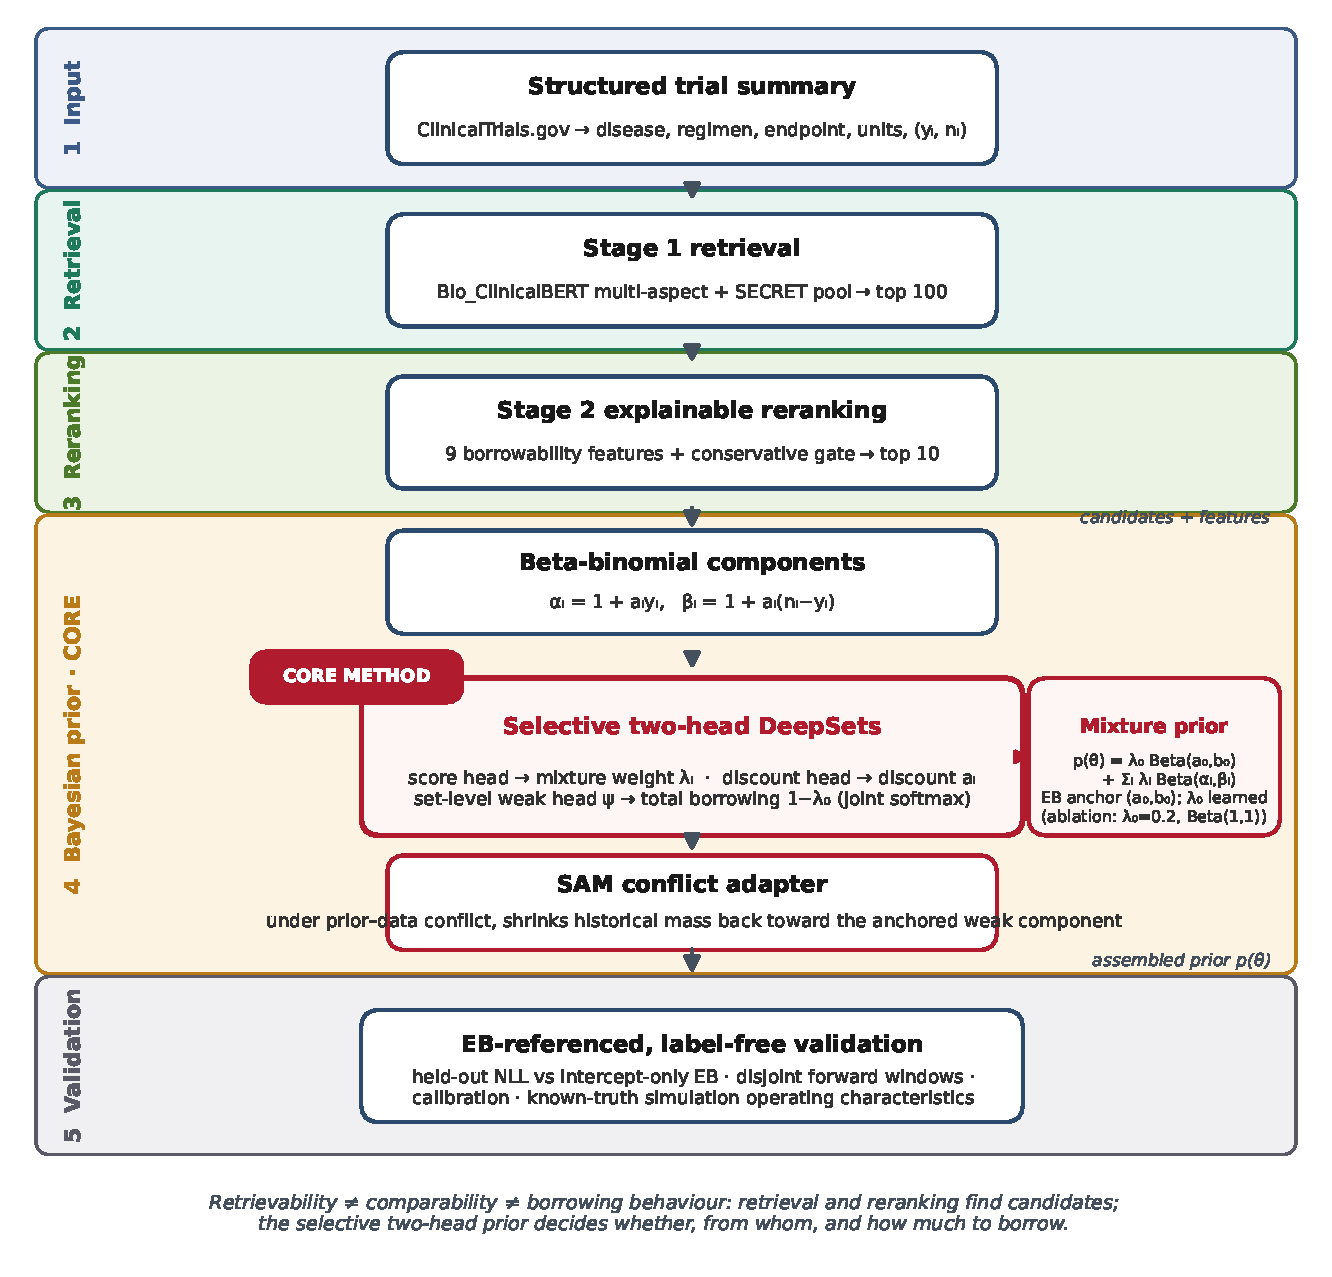
\includegraphics[width=\textwidth]{F7_pipeline_schematic}
  \caption{\textbf{Pipeline overview.} Schematic of the borrowability
  pipeline: ClinicalTrials.gov parsing, structured trial summary, Stage~1
  retrieval with the SECRET-inspired section pool, explainable Stage~2
  reranking, beta-binomial mixture components, and selective two-head DeepSets
  weighting --- separating the mixture weight $\lambda$ from the
  borrowed-size discount $a$, with a set-level head that learns the
  total borrowing $1-\lambda_0$ per query --- followed by the historical
  mixture-mass cap that completes the final design. The SAM conflict
  adapter (dashed) is a sensitivity analysis only and is not part of the
  final design.}
  \label{fig:pipeline}
\end{figure}

We are explicit about what this evidence can and cannot establish. No corpus of
expert borrowability labels exists for oncology registry trials, so we make no
claim to adjudicate clinical suitability, and every result below is a
calibration statement rather than a clinical one. In place of labels we assemble
a retrospective evidence package: leakage-controlled pseudo-queries, in which
completed trials are replayed with their outcomes hidden; held-out beta-binomial
predictive negative log-likelihood (NLL) as a proper scoring rule; true-date
temporal validation using ClinicalTrials.gov completion dates rather than NCT
numeric proxies; simulation operating characteristics reported following
established reporting standards for simulation studies [25]; comparison against
weak-only, rule-based, power-prior-, MAP- and UIP-style baselines
[3,~4,~19]; and feature ablation. The contributions
are therefore fivefold, and we foreground the second and third as the central
methodological novelty: (i) the retrieve $\rightarrow$ rerank $\rightarrow$
borrow pipeline linking registry retrieval to prior construction;
(ii)~\emph{the selective two-head DeepSets model, which learns, for each
individual donor trial, a mixture weight
and a separate information discount, and, through a set-level head, the
per-query total borrowing fraction, all as permutation-invariant functions of
the whole retrieved set, so that donor selection, per-donor information size,
and whether to borrow at all become decoupled, learnable quantities} --- with
the evidence for each decision graded explicitly: the architecture
permits separate per-source discounting, but in the final selective model
the learned discount response was empirically flat (Supplement~S4), and
the observed gain is attributable primarily to the EB anchor and the
set-level total-borrowing head; the set-level decisions
(when to borrow, and how much in total, under an explicit cap) are the ones
our data support, while donor-level discrimination and an active
per-source discount remain architectural
capabilities that are not empirically demonstrated;
(iii)~\emph{the capped final design and its assessment frames}: a
historical mixture-mass cap of $0.5$ fixed before the cap analyses, a
corpus-estimated donor--query
drift distribution --- to our knowledge the first such measurement on
registry ORR data --- used as the mixing measure of an exploratory
corpus-specific decision analysis with a tolerated pointwise inflation
ceiling, an
independent large validation batch so that threshold selection and
error-rate assessment never share simulation data, size-matched power
comparisons so liberality cannot masquerade as benefit, and worst-case
reporting alongside, in explicit acknowledgement that strict unrestricted
type~I control forfeits all power gains from borrowing in one-parameter
settings of this kind [28];
(iv) an EB-referenced, leakage-partitioned, availability-tiered evaluation
protocol that scores every design-time prior against an intercept-only
empirical-Bayes reference, assesses outcome-adaptive layers (a transparent
SAM-style conflict adapter) by known-truth simulation, and puts the
availability-consistent primary analysis first; and
(v) an honest empirical accounting, of independent cautionary value, of how
much candidate-level borrowing adds over marginal priors on registry-scale
oncology data --- nothing yet on decision-time-available data, a small
mixture-average gain concentrated where donors are approximately
exchangeable in simulation, and an upper-bound gain concentrated where the
retrieved candidate set is information-rich. We draw the
boundary plainly: automated retrospective evidence of this kind supports method
development and pre-specification, not clinical borrowing decisions, which
continue to require disease-specific expert review. The remainder of the paper
is organised as follows. Section~2 describes the data, the three stages, and
the evaluation protocol; Section~3 sets up the gold-standard and
external-control simulations; Section~4 reports the EB-referenced borrowing
comparisons, forward validation, calibration diagnostics, simulation operating
characteristics, and worked case studies; Section~5 discusses the
implications, the relationship to existing adaptive-borrowing methods, and the
limitations of the approach.


\subsection*{Positioning relative to existing adaptive-borrowing methods}

We state at the outset what is and is not new here, because the individual
statistical components of this framework have close precedents and we do not
wish to claim otherwise.

Per-source adaptive weights driven by the information content of each
historical dataset are the defining feature of the unit information prior (UIP)
of Jin and Yin [19], which also requires only summary statistics. Deciding how
much to borrow from covariates without looking at the current outcome --- what
we call prospective allocation --- is the basis of propensity-score integrated
power priors and related proactive overlap-based borrowing [20,~21]. Dynamic
borrowing from trial-level summaries with covariates has been developed as a
Bayesian model-averaging construction [22], and covariate-adjusted dynamic
borrowing has been studied in this journal [23]. Outcome-dependent conflict
adaptation is the SAM prior [11]. The permutation-invariant set architecture we
use is DeepSets [24], applied here with two output heads; multi-head networks
are standard practice. Taken individually, therefore, neither a per-source
borrowed sample size, nor prospective allocation, nor a two-head set network
constitutes a new statistical method, and we do not present them as such.

What we did not find a precedent for is the integration: a \emph{learned set
function} that maps a large, retrieval-derived candidate pool of free-text
trial records to both a mixture allocation and a per-source effective
sample-size discount, trained end-to-end against held-out predictive
likelihood. Within that integration, two concrete methodological increments are,
to our knowledge, new. \emph{First}, we \emph{decouple} the two borrowing
decisions that existing dynamic-borrowing priors tie together: a single
permutation-invariant network emits, per donor, a mixture weight $\lambda_i$
(which donor) \emph{and} a separate borrowed-size discount $a_i$ (how
much information), so that ``which'' and ``how much'' are learned independently
rather than through one shared weight. \emph{Second}, we add a design-time,
\emph{outcome-free} set-level conflict signal that---unlike SAM or UIP-JS, which
require the current outcome---is available before the trial reads out, and which
is what makes the learned discount head responsive to comparability in the
\emph{fixed-budget} architecture; in the final selective model even that
role disappears --- the discount response is empirically flat and
adaptivity migrates to the set level (Supplement~S4) --- so we no longer
claim an active per-source discount as a working mechanism of the final
design. The contribution we defend is this integration together with a
gold-standard simulation protocol that makes the borrowing decision itself ---
not merely the resulting estimate --- an object of evaluation with known truth.
We are candid that, measured only by donor ranking, these increments are modest,
and we report them as such---including where they do not help; their value is
that they make an otherwise inert learned discount function work, and that they
operate entirely at design time.

% ---------------------------------------------------------------------
\section{Methods}

\subsection{Method overview}
\label{sec:overview}
The pipeline converts a query oncology trial into a Bayesian mixture prior for
its endpoint in three stages (Figure~\ref{fig:pipeline} and
Algorithm~\ref{alg:pipeline}). \emph{Stage~1 (retrieve)} uses existing retrieval
backends to pull a high-recall pool of candidate historical trials from
ClinicalTrials.gov. \emph{Stage~2 (rerank)} scores each candidate on nine
auditable, borrowing-relevant features and applies a conservative clinical gate
that removes endpoint-incompatible or unusable candidates. \emph{Stage~3
(borrow)} turns each surviving candidate into a beta-binomial historical
component and combines the components into a mixture prior, setting each
candidate's mixture weight and borrowed-size discount either by a
transparent rule or by the learned two-head DeepSets model. Of these parts,
Stage~1 retrieval and the optional SAM adapter reuse published tools
[11,~12,~13,~14,~24]; the novel element is Stage~3's learned set function, which
maps a large free-text candidate pool jointly to a per-donor allocation and a
per-donor information size. The remainder of this section describes the data
(Section~\ref{sec:data}), the three stages, and the label-free evaluation
protocol (Section~\ref{sec:eval}).

\begin{algorithm}[htbp]
\caption{Retrieve $\rightarrow$ rerank $\rightarrow$ borrow. Steps marked
(existing) reuse published tools; the step marked (new) is this paper's core
contribution.}
\label{alg:pipeline}
\small
\textbf{Input:} query trial $q$ with its endpoint outcome hidden; corpus of
historical trials. \quad
\textbf{Output:} Bayesian mixture prior for the query endpoint.
\begin{enumerate}[nosep,leftmargin=1.9em,label=\arabic*.]
\item \textbf{Stage 1 --- retrieve} \emph{(existing)}: encode $q$ and score the
corpus with the chosen backend (hashing / ClinicalBERT [13] / Trial2Vec [12] /
SECRET pool [14]); keep the top-$M$ candidates.
\item \textbf{Stage 2 --- rerank} \emph{(existing components, assembled here)}:
compute the nine borrowing features $x_i$ for each candidate; apply the
conservative clinical gate $\mathrm{gate}_i$; keep the top-$K$.
\item \textbf{Stage 3 --- borrow} \emph{(new)}: for each surviving candidate
$i$, extract the endpoint observation $(y_i, n_i)$; the selective two-head
DeepSets model maps the whole set $\{x_j\}$ to a candidate score $z_i$
\emph{and} a separate borrowed-size discount $a_i$, while a set-level head
emits a weak-component logit $z_0$ from the pooled set context; a joint
softmax over $[z_0, z_i + \log \mathrm{gate}_i]$ yields the weights
$(\lamz, \lambda_i)$, so the total borrowing $1-\lamz$ is learned per query.
Build each beta component $\mathrm{Beta}(1+a_i y_i,\ 1+a_i(n_i-y_i))$.
\item Assemble the mixture prior
$p(\theta) = \lamz\,\mathrm{Beta}(a_0,b_0) + \sum_i \lambda_i\,\mathrm{Beta}(\alpha_i,\beta_i)$,
with $(a_0,b_0)$ the empirical-Bayes anchor fitted to training-era queries
(flat $(1,1)$ with fixed $\lamz=0.2$ in the fixed-budget ablation).
\item \emph{(sensitivity analysis; not part of the final design)}
\textbf{SAM adapter} \emph{(existing [11])}: if the
observed outcome conflicts with the historical mixture relative to the anchored
weak component, down-weight historical mass and return it to that weak
component.
\end{enumerate}
\end{algorithm}

\noindent The candidate budgets $M$ (default $100$) and $K$ (default $10$) are
illustrative values used for demonstration; both are configurable pipeline
parameters rather than fixed constants of the method.

\subsection{Data source and structured trial summaries}
\label{sec:data}
The pipeline uses local ClinicalTrials.gov oncology trial records. Each record
is parsed into a structured summary that includes disease context, patient
population, regimen, endpoint text, follow-up or time-frame text, eligibility
criteria, result availability, extractable endpoint observations, and red
flags. The structured summary is the shared representation used by retrieval,
reranking, candidate feature construction, and temporal validation.

True date metadata are extracted separately to support temporal validation.
The date extraction module reads newer ClinicalTrials.gov API-style records
and local legacy exported JSON structures. It extracts primary completion
date, completion date, results first posted date, and start date. Dates are
normalized with precision labels (day, month, year, missing, unparseable).
Month-only dates are mapped to deterministic mid-month anchors for sorting
while retaining the precision label. Primary completion date is preferred for
temporal sorting, followed by completion date, results first posted date,
start date, and NCT numeric proxy only when true date metadata are
unavailable. In the current extract this module produced true
ClinicalTrials.gov temporal metadata for 7{,}173 oncology trials: primary
completion date was available for all 7{,}173 trials (6{,}631 at day-level and
542 at month-level precision), and start and results-first-posted dates were
available for all records, enabling temporal analyses based on primary
completion dates rather than NCT numeric proxy ordering.

\subsection{Leakage-controlled pseudo-query construction}
Completed trials are used retrospectively as pseudo-queries. For each
pseudo-query, the query outcome is hidden from retrieval and reranking.
Candidate selection uses only structured trial information and historical
candidate records. The held-out pseudo-query endpoint observation is used only
for retrospective predictive evaluation. Pipeline-result rows used for
training or evaluation require explicit leakage-control metadata and held-out
query outcomes; rows lacking those fields are rejected by the training and
evaluation code.

The current empirical evidence package focuses on objective response rate
(ORR) pseudo-queries, because ORR endpoint observations are the most commonly
extractable from ClinicalTrials.gov result tables in this prototype. Extending
the full retrieval and two-head pipeline to other endpoints requires
per-endpoint pseudo-query construction and is treated as a future validation
target.

\subsection{Stage 1 retrieval and SECRET pool construction}
Stage~1 retrieval identifies high-recall candidate historical trials. The
implemented backends include hashing, ClinicalBERT-style embeddings [13],
optional Trial2Vec-style retrieval [12], and SECRET-style section retrieval
[14]. Trial2Vec-style
retrieval depends on local package, model, and index availability and was
treated as an optional backend rather than a required component of the present
evidence package. The SECRET-style path is a deterministic section-weighted
implementation that emphasizes borrowing-relevant trial sections rather than
title similarity alone; it should be interpreted as a SECRET-inspired pool
construction path, not a complete reproduction of the SECRET method [14]. Candidate
pools produced by Stage~1 are then available for Stage~2 reranking and
endpoint observation extraction.

The ClinicalBERT backend encodes five weighted aspect views of each trial ---
disease and population (weight $0.30$), intervention ($0.25$), endpoint
($0.20$), design ($0.15$), and results and safety ($0.10$) --- using
mean-pooled \texttt{emilyalsentzer/Bio\_ClinicalBERT} token embeddings
(maximum sequence length 256) and retrieves candidates by cosine similarity of
the weighted aspect representation. Bio\_ClinicalBERT is a biomedical language
model rather than a model trained specifically for trial-to-trial similarity,
so it is used here only as a high-recall candidate-discovery backend. Stage~1
returns up to 100 candidates per query, of which the top 10 reranked candidates
are carried forward to endpoint extraction and mixture-prior construction; these
two counts are illustrative defaults chosen for demonstration and are
configurable pipeline parameters, not fixed constants of the method.

\subsection{Explainable Stage 2 reranking}
\label{sec:rerank}
Stage~2 reranking scores candidate pairs using borrowing-relevant features.
The current feature schema includes overall similarity, disease match, regimen
match, endpoint match, follow-up match, eligibility match, result quality,
negative red-flag severity, and information size. These features are intended
to make the basis for candidate prioritization auditable. They are not expert
labels and are not interpreted as final clinical borrowing decisions. The
rule-based raw weight for a component combines clinical gating, discounting,
similarity, and information size:
\begin{equation}
w_i \;=\; \mathrm{gate}_i \cdot a_i \cdot \frac{\max(\mathrm{overall}_i,0)}{100}
\cdot \log(1+n_i).
\end{equation}
Here $\mathrm{overall}_i$ is the Stage~2 overall similarity on a $0$--$100$
scale and $n_i$ the candidate endpoint denominator; the individual reranking
dimensions are scored on a $0$--$5$ scale. The gate is deliberately
conservative: $\mathrm{gate}_i = 0$ when the endpoint match falls below $1.5$
on the $0$--$5$ scale or result usability is zero; otherwise
$\mathrm{gate}_i = 1$, multiplied by $0.2$ for severe disease mismatch (disease
match below $1.5$), by $0.6$ for moderate disease mismatch (below $2.5$), and
by $0.5$ when a low-quality red flag is present. Endpoint-incompatible
candidates, candidates without usable result data, severe disease mismatch, and
red flags can therefore remove or downweight a candidate before any learned
model assigns mixture mass. This design prevents retrospective predictive fit
from overriding basic endpoint, result, and clinical-compatibility checks. The
raw weights $w_i$ are not used as final quantities: they are normalized across
candidates into the mixture weights $\lambda_i$ of
Section~\ref{sec:mixture}, and in the learned pipeline the two-head model
replaces this rule-based weighting entirely.

\subsection{Endpoint observations and beta-binomial components}
For candidate $i$, the pipeline extracts an endpoint observation
$(y_i,n_i)$ when a compatible result table is available, where $y_i$ is the
candidate endpoint response or event count and $n_i$ is the candidate endpoint
denominator. Candidates without compatible endpoint observations can still be
retrieved and reranked, but they do not contribute a historical beta-binomial
component. When an endpoint observation is usable, the candidate contributes a
beta component
\begin{equation}
\alpha_i = 1 + a_i y_i, \qquad
\beta_i  = 1 + a_i (n_i - y_i),
\end{equation}
where $a_i$ is an borrowed-size discount that controls the amount of
information borrowed inside the candidate beta component.

\subsection{Mixture prior, mixture weights, and borrowed-size discounts}
\label{sec:mixture}
The present construction targets \emph{binary} endpoints---an endpoint expressed
as a response or event count out of a denominator, such as ORR---so $\theta$ is
a response probability and each historical component is beta-binomial;
extension to time-to-event and continuous endpoints is left to future work. The
prior for the response probability $\theta$ is represented as a weak
component plus historical components:
\begin{equation}
p(\theta) \;=\; \lamz\,\mathrm{Beta}(\theta\mid a_0,b_0)
\;+\; \sum_i \lambda_i\,\mathrm{Beta}(\theta\mid \alpha_i,\beta_i),
\end{equation}
where $(a_0, b_0)$ parameterizes the weak (anchor) component. The rule-based
prototype fixes $\lamz = 0.2$ and a flat anchor
$(a_0,b_0) = (1,1)$: raw historical weights are normalized to the remaining
prior mass $1-\lamz$, and if all raw historical weights are zero the prior
falls back to a weak-only form with $\lamz = 1$. Two consequences of that
fixed budget matter for everything that follows. First, whenever \emph{any}
candidate passes its gate, a constant $80\%$ of prior mass is forced onto the
retrieved candidates, however weak they are. Second, the flat anchor places
the fallback mass on a prior with mean $0.5$, far from the marginal ORR
distribution of oncology trials. The selective learned model of
Section~\ref{sec:twohead} removes both restrictions: the anchor becomes an
empirical-Bayes fit and the total borrowing becomes a learned, per-query
quantity. The component weight $\lambda_i$ and the
discount $a_i$ are conceptually distinct throughout: the former controls
allocation across mixture components, whereas the latter controls the nominal
information size inside a component. When model-based weights are applied, the
implementation retains rule-based weights and rule-based beta parameters for
auditability.

\subsection{Selective two-head DeepSets model for weights, discounts, and total borrowing (core method)}
\label{sec:twohead}
The selective two-head DeepSets model is the central methodological
contribution of this work. Classical robust priors assign a single pooled
weight to all historical evidence and set the borrowing discount separately or
by fixed rule; our own earlier fixed-budget architecture learned
candidate-specific weights and discounts but still forced a constant total
borrowing fraction. Here \emph{three} quantities are learned as functions of
design-time borrowability features, permutation-invariant in the retrieved
candidate set: the per-candidate mixture weight $\lambda_i$, the per-candidate
information discount $a_i$, and --- through a set-level head that places the
weak component inside the same softmax --- the per-query total borrowing
fraction $1-\lamz$. The paired
benchmarks of the primary analysis
(Section~\ref{sec:primary-results}), the upper-bound tiers
(Sections~\ref{sec:headtohead-results}
and~\ref{sec:forward-results}), and the calibration analysis at the end of
Section~\ref{sec:forward-results} evaluate this model (\texttt{selective}) against
the empirical-Bayes reference and against the fixed-budget predecessor
(\texttt{two\_head}), which is retained as an ablation; \texttt{selective\_sam}
denotes the combination with the outcome-adaptive SAM conflict adapter of
Section~\ref{sec:sam}.

\paragraph{Candidate features.} Each candidate $i$ is represented by a
nine-dimensional feature vector
\begin{equation}
x_i = \big[\, s_i,\ d^{\mathrm{dis}}_i,\ d^{\mathrm{reg}}_i,\ d^{\mathrm{end}}_i,\
d^{\mathrm{fu}}_i,\ d^{\mathrm{elig}}_i,\ q^{\mathrm{res}}_i,\
-\,\mathrm{rf}_i,\ \log(1+n_i) \,\big],
\end{equation}
where $s_i$ is the Stage~2 overall similarity divided by $100$, each match term
$d^{\bullet}_i$ is the corresponding $0$--$5$ dimension score divided by $5$,
the red-flag severity $\mathrm{rf}_i \in [0,1]$ enters with a negative sign, and
$\log(1+n_i)$ encodes information size on a diminishing-returns scale. These are
the same auditable borrowability dimensions used by the rule reranker
(Section~\ref{sec:rerank}), so the learned and rule priors operate on identical inputs and
differ only in how those inputs are combined.

\paragraph{DeepSets backbone.} A shared per-candidate encoder $\phi$ (a
one-hidden-layer network of width $16$ with a ReLU activation) maps each $x_i$
to a hidden vector. The set context is the mean of $\phi$ over the retrieved
candidate set, $c = \tfrac{1}{K}\sum_j \phi(x_j)$; this permutation-invariant
pooling is the DeepSets construction and makes every candidate score
independent of candidate ordering and dependent on the whole candidate pool
rather than the candidate in isolation. A function $\rho$ combines the
candidate embedding $\phi(x_i)$ with the pooled context $c$ to yield a raw score
$z_i$, so that borrowing ``this candidate relative to the rest of the set'' is
expressible --- the property a single pooled prior cannot represent.

\paragraph{Head 1 --- mixture allocation, jointly with the weak component.}
A set-level head maps the pooled context $c$ to a weak-component logit
$z_0 = \psi(c)$ (a one-hidden-layer network of width $16$), and allocation is
a single softmax over the weak component and the gated candidates,
\begin{equation}
\lamz = \frac{\exp(z_0)}{\exp(z_0) + \sum_j \exp(z_j)\,\mathrm{gate}_j},
\qquad
\lambda_i = \frac{\exp(z_i)\,\mathrm{gate}_i}{\exp(z_0) + \sum_j \exp(z_j)\,\mathrm{gate}_j},
\end{equation}
so candidates with $\mathrm{gate}_i = 0$ (the conservative clinical gate of
Section~\ref{sec:rerank}) are masked entirely and
$\lamz + \sum_i \lambda_i = 1$ with $\lamz$ free to vary per query. When the
candidate logits are weak relative to $z_0$ the model borrows little; when the
set is information-rich it borrows more --- this is the selectivity mechanism,
and Section~\ref{sec:triage-results} verifies that the learned $\lamz$ in fact
tracks a pre-specified design-time information measure. If every gate is zero
the prior collapses to weak-only ($\lamz = 1$). The fixed-budget predecessor
is recovered exactly by replacing $\exp(z_0)$ with
$\tfrac{\lamz^{\mathrm{fix}}}{1-\lamz^{\mathrm{fix}}}\sum_j \exp(z_j)\,\mathrm{gate}_j$
for $\lamz^{\mathrm{fix}} = 0.2$, which is how the \texttt{two\_head} ablation
is defined.

\paragraph{Empirical-Bayes anchor.} The weak component is
$\mathrm{Beta}(\hat a_0, \hat b_0)$ with $(\hat a_0, \hat b_0)$ fitted by
beta-binomial maximum likelihood to the training-era query outcomes only ---
the training split for the primary fit ($\mathrm{Beta}(0.68, 1.70)$, mean
$0.28$, nominal information $2.4$ patients), and past-only data at each cutoff
for the forward refits. Declining to borrow therefore means falling back to
the marginal ORR distribution of comparable-era trials rather than to a flat
prior with mean $0.5$. The identical EB prior, used alone, is the reference
baseline of Section~\ref{sec:eval}.

\paragraph{Head 2 --- information discount.} The second head outputs a
per-candidate discount $a_i \in (0,1]$, which reconstructs that candidate's beta
component as $\alpha_i = 1 + a_i y_i$ and $\beta_i = 1 + a_i(n_i - y_i)$, so
that $a_i n_i$ is the component's nominal borrowed sample size.
Separating $a_i$ (how much information a borrowed component carries) from
$\lambda_i$ (how much mixture mass it receives) is a key modeling choice:
allocation and information size are learned independently rather than tied to a
single weight. If a checkpoint has no discount head, the rule discount and its
beta parameters are used.

\paragraph{Training objective.} The model is trained end-to-end by minimizing,
over training pseudo-queries, the combined loss
\begin{equation}
\mathcal{L} = \mathcal{L}_{\mathrm{pred}}
+ \rho\,\mathrm{KL}(\lambda^{\mathrm{rule}}\,\|\,\lambda^{\mathrm{model}})
+ \eta\,\mathcal{L}_{\mathrm{list}}
+ \mathcal{L}_{\mathrm{ESS}},
\end{equation}
whose terms are: (i)~the primary predictive loss $\mathcal{L}_{\mathrm{pred}}$,
the mean training-outcome beta-binomial mixture predictive NLL under the
EB-anchored selective mixture (Section~\ref{sec:eval});
(ii)~a Kullback--Leibler term with weight $\rho = 0.1$ pulling the
\emph{normalized} candidate allocation $\lambda_i / \sum_j \lambda_j$ toward
the normalized rule allocation --- a mild regularizer that stabilizes relative
allocation on small data without penalizing or rewarding the learned total
borrowing $\sum_i \lambda_i$; (iii)~an optional
listwise allocation term with weight $\eta$ (disabled by default, $\eta = 0$)
whose target $t_i = \mathrm{softmax}_i(r_i/T)$ is built from each candidate's
relative log predictive
$r_i = \log P(y_0\mid n_0,\alpha_i,\beta_i) - \log P(y_0\mid n_0,1,1)$, giving a
within-candidate-set signal for which donors best explain the training outcome;
and (iv)~a borrowed-information penalty
$\mathcal{L}_{\mathrm{ESS}} = 10^{-4}\,\max\!\big(\sum_i \lambda_i a_i n_i - \mathrm{ESS_{cap}},\,0\big)^2$
with $\mathrm{ESS_{cap}} = 100$ on the weighted nominal borrowed sample size
(Section~\ref{sec:eval} discusses why this quantity is a nominal summary
rather than a mixture-prior effective sample size). Held-out evaluation uses
only the pure predictive NLL and excludes all regularizers. Optimization used
Adam (learning rate $0.01$) for $100$ epochs with hidden width $16$; the model
was fit on an $80\%$ split of the pseudo-queries (seed $20260603$) and, for the
forward analysis with past-only refits at each temporal
cutoff (Section~\ref{sec:forward-results}).

\paragraph{Inference.} For a new query with no available outcome, Stages~1--2
produce the candidate set and features; the model outputs $\lambda_i$ and $a_i$,
the mixture prior is assembled, and the rule-based $\lambda^{\mathrm{rule}}$ and
beta parameters are retained alongside the learned values so that reports can
compare rule-based versus learned prior mass. The SAM conflict adapter
(Section~\ref{sec:sam}) is applied afterward only when the current outcome is available
and conflict adaptation is requested.

\subsection{SAM-style prior-data conflict adaptation}
\label{sec:sam}
A conflict adapter in the style of the self-adapting mixture (SAM)
prior [11] is evaluated as a named sensitivity analysis for the
\emph{uncapped} selective prior. It is not part of the final design
(Section~\ref{sec:cap}): the mixture-mass cap there achieves the same
worst-case protection at lower power cost, and the simulation reports both
so the redundancy is measured rather than asserted.
The adapter downweights historical components when the pseudo-query outcome
conflicts with the prior predictive distribution. Let
$P_{\mathrm{weak}} = P(y_0 \mid n_0, a_0, b_0)$ be the predictive of the
prior's own weak component at the held-out outcome---the flat
$\mathrm{Beta}(1,1)$ for the rule and fixed-budget priors, the EB anchor for
the selective prior---and
$P_{\mathrm{hist}} = \sum_i \tilde\lambda_i\,P(y_0 \mid n_0, \alpha_i, \beta_i)$
the historical-informative predictive, where $\tilde\lambda_i$ are the active
candidate weights renormalized to sum to one. With the conflict ratio
$R = P_{\mathrm{hist}}/P_{\mathrm{weak}}$, the borrowing multiplier is $1$ when
$R \ge 1$ and $R^{\tau}$ when $R < 1$ (temperature $\tau = 1$); each active
candidate weight is scaled by this multiplier and the removed mass is returned
to that same weak component, so a SAM-adjusted selective prior collapses
toward the EB anchor rather than toward a flat prior. Borrowing is thus preserved when the historical prior is
at least as consistent with the data as the weak prior, and progressively
withdrawn as prior-data conflict grows. In this manuscript, SAM adaptation is
interpreted as a transparent conflict-sensitivity mechanism, not as a regulatory
qualification procedure. Because SAM uses the observed (pseudo-)query outcome to
assess prior-data conflict, it cannot be used to pre-select historical evidence
before the trial outcome is observed; any applied use would require embedding it
within a pre-specified dynamic-borrowing design.

Two evaluation consequences follow and are enforced throughout the paper.
First, a same-outcome predictive score of a SAM-adjusted prior is not a proper
out-of-sample score of a design-time prior: the adapter has already shifted
mass toward whichever side of the mixture better fits the outcome being
scored, so part of any NLL advantage is mechanical. SAM-adjusted rows are
therefore segregated into an explicitly labelled \emph{outcome-adaptive} block
of the results tables, are never compared as equals with design-time priors,
and are never the basis of a performance claim. Second, the legitimate
evaluation of an outcome-adaptive rule is frequentist and prospective: the
known-truth simulation of Section~\ref{sec:simulation}, in which SAM's effect
on type~I error, power, coverage, and trigger behaviour is measured over
replicates against the generating truth. The selective architecture of
Section~\ref{sec:twohead} supplies the design-time counterpart of the same
instinct: it withholds borrowing using candidate-set features available before
the outcome exists, rather than the outcome itself.

\subsection{Historical mixture-mass cap and the final design}
\label{sec:cap}
The selective prior of Section~\ref{sec:twohead} is a mixture
$\pi = \lambda_0\,\mathrm{Beta}(a_0,b_0) + \sum_i \lambda_i\,
\mathrm{Beta}(\alpha_i,\beta_i)$ with $\lambda_0 + \sum_i \lambda_i = 1$;
call $m = \sum_i \lambda_i$ its \emph{historical mass}. The historical
mixture-mass cap (``the cap'' hereafter) is the projection
\[
  \lambda_i \;\leftarrow\; \lambda_i \cdot \min\!\big(1,\; c/m\big),
  \qquad
  \lambda_0 \;\leftarrow\; 1 - \textstyle\sum_i \lambda_i ,
\]
so that historical components can never jointly carry more than $c$ of the
\emph{prior mixture probability}; the excess returns to the anchored weak
component. The cap is a
deterministic function of the design-time prior, applies identically in
simulation and at real-data scoring, requires no retraining, and preserves
the learned \emph{allocation} across donors while bounding the learned
\emph{total}. We are precise about what it does and does not bound: it caps
component probability, \emph{not} information or influence --- a precise
historical component at mass $0.5$ can still dominate the posterior when
the data favour it, so $c = 0.5$ must not be read as ``at most half the
information,'' and the equal-footing motivation (historical evidence
should not carry more prior probability than the anchored representation
of the current trial's own context, in the spirit of Pocock's caution
[1]) is a heuristic, not a theorem. The cap's actual protection is
therefore measured rather than asserted: posterior-influence diagnostics
on real data and precision-stress simulations (donor arm sizes $\times 4$;
anchor precision $\times 4$ and $\times 1/4$) are reported in
Section~\ref{sec:goldsim-results}. The value $c = 0.5$ was fixed before
any of the round-4 cap analyses (we do not call it a priori in the strict
sense: it was chosen during a revision cycle, after earlier rounds of data
contact); the full cap--power--error curve over $c \in \{0.1,\dots,0.9\}$
(Section~\ref{sec:goldsim-results}) is reported so the reader can see what
the choice trades away, and neighbouring caps are carried as sensitivity
analyses in every real-data tier.

\paragraph{The final design.} The complete specified design of this paper is
the \emph{capped selective prior}: selective two-head allocation
(Section~\ref{sec:twohead}), EB anchor, mixture-mass cap $c = 0.5$, and a
success threshold calibrated as specified in
Section~\ref{sec:goldsim}. It contains no outcome-adaptive component:
the SAM adapter of Section~\ref{sec:sam} is measured to be largely redundant
under the cap (Section~\ref{sec:goldsim-results}) and is reported only as a
sensitivity analysis for the uncapped prior. Wherever this paper says
``final design'' it means exactly this object; the uncapped selective prior
is its ablation.

\subsection{Prospective set-level conflict signal}
\label{sec:prospective}
The nine reranking dimensions all describe design and surface comparability:
disease, regimen, endpoint definition, follow-up window, eligibility, result
quality, red flags and information size. None of them carries any information
about whether a candidate's \emph{observed outcome} is discrepant. We therefore
add one further input, computed from the donors alone.

For candidate $i$ with observed rate $r_i = y_i/n_i$, let $m_{-i}$ be the
sample-size-weighted median of $\{r_j : j \neq i\}$ and let $s_{-i}$ be the
corresponding weighted median absolute deviation, scaled by $1.4826$ and
floored at $0.02$. The set-level conflict signal is
\[
  g_i \;=\; \min\!\left(\frac{|r_i - m_{-i}|}{s_{-i}},\; 8\right).
\]
The leave-one-out construction matters: including candidate $i$ in the
consensus it is measured against would let a single dominant donor define its
own reference and mask the outlier we are trying to detect.

Crucially $g_i$ uses only outcomes that are already published for the candidate
trials; the query trial's outcome never enters. The signal is therefore
available at design time, which distinguishes it from SAM (Section~\ref{sec:sam}) and
from UIP-JS [19], both of which compute their conflict measure against the
current trial's data. We report $g_i$-augmented and $g_i$-free versions of the
same model throughout, so that its contribution can be read directly.

\subsection{Evaluation without expert borrowability labels}
\label{sec:eval}
Expert borrowability labels were unavailable. Evaluation therefore used
internal retrospective and simulation evidence, organised around three design
decisions.

\paragraph{The empirical-Bayes reference.} Every real-data comparison is
judged against the intercept-only EB prior of Section~\ref{sec:twohead}: a
single $\mathrm{Beta}(\hat a_0,\hat b_0)$ fitted by beta-binomial maximum
likelihood to training-era query outcomes, using no candidate information
whatever. This reference exists because a flat $\mathrm{Beta}(1,1)$ is a straw
man for oncology ORR --- much of any borrowing method's apparent gain over it
comes merely from learning that response rates are usually well below $0.5$.
A borrowing pipeline earns its complexity only by what it adds \emph{beyond}
the marginal outcome distribution. We additionally report a
disease-stratified EB variant (per-primary-site fits for strata with at least
$40$ training queries, global fallback otherwise) as a second, stronger
marginal reference.

\paragraph{Design-time versus outcome-adaptive priors.} Priors fixed before
the current outcome is seen (EB, stratified EB, rule, fixed-discount,
commensurate-, MAP- and power-prior-style, robust-MAP, the fixed-budget
two-head, and the selective model) are scored by held-out predictive NLL, a
strictly proper score for them. Outcome-adaptive layers (SAM variants), whose
same-outcome scores are partly mechanical (Section~\ref{sec:sam}), appear only
in a separately labelled table block and are assessed by simulation operating
characteristics.

\paragraph{Outcome roles and terminology.} Each pseudo-query outcome plays
exactly one of four roles, named consistently throughout: a \emph{masked}
outcome is hidden from retrieval and reranking during feature construction
(true of every query); a \emph{training} outcome is additionally used to fit
model parameters or EB anchors; a \emph{validation} outcome steers no fitting
and is scored by a model whose training set excluded it --- the held-out $20\%$
test split (random, seed $20260603$) and the forward windows below; a
\emph{development-set} score is one computed over a set that includes training
outcomes (reported only for completeness, always labelled). Forward validation
uses \emph{disjoint} future windows: each window $(c_k, c_{k+1}]$ of primary
completion dates is scored once, by the model and EB anchor refit on data
up to $c_k$ only, so no trial is evaluated twice and no future information
enters any fit.

The evidence layers are: held-out beta-binomial predictive NLL against the EB
reference; disjoint-window forward validation with past-only refits;
predictive calibration diagnostics; simulation operating characteristics;
borrowing baseline head-to-head comparisons; feature ablation and
section-weight sensitivity; and software verification through focused and full
unit-test runs. Two pre-specified real-data subgroup analyses accompany the
aggregate comparisons: the design-time measure of candidate-set
information $I$,
defined as $\sum_i \mathrm{gate}_i\, a^{\mathrm{rule}}_i n_i$ and
dichotomised at $I \ge 8$
(fixed from an exploratory analysis on the earlier temporal windows before the
final window was examined), and the learned total borrowing itself as a
descriptive diagnostic. All other subgroup splits are labelled exploratory.
A terminological caution applies to information summaries: for a mixture
prior, $\sum_i \lambda_i a_i n_i$ is a \emph{weighted nominal borrowed sample
size}, not the prior's effective sample size in the sense of Morita et al.;
mixture information depends on component separation and the weak-component
mass, so we use the nominal quantity only as a bookkeeping summary and label
it accordingly.

All results are interpreted as retrospective predictive calibration or
simulation evidence. They do not establish expert-level borrowability of
individual candidates. Table~\ref{tab:datasets} summarizes the evaluation
datasets, sample sizes, train/test splitting, leakage status, and endpoint
scope of each analysis so that the different evidence layers are not conflated.

\begin{table}[htbp]
\centering
\small
\caption{Evaluation datasets and evidence layers. ``Leakage-free'' marks
analyses in which no evaluated model saw the scored query during fitting;
``model-development'' marks the retrospective head-to-head, in which closed-form
priors involve no outcome or fitting leakage by construction but the learned rows include queries
that contributed to model development. All primary analyses use objective
response rate (ORR) pseudo-queries.}
\label{tab:datasets}
\begin{tabular}{p{0.235\textwidth}p{0.135\textwidth}p{0.30\textwidth}p{0.19\textwidth}}
\toprule
Analysis & Size & Split / leakage status & Endpoint scope \\
\midrule
EB reference priors & fits on 1{,}126 train / past-only pools & Intercept-only and disease-stratified beta-binomial MLE; no candidate information & ORR \\
Borrowing head-to-head + calibration & held-out split 281; development set 1{,}407 & Outcome/fitting leakage controlled for all methods (donor availability at decision time not enforced; Section~\ref{sec:eval}); development-set columns include training outcomes for learned rows and are labelled & ORR \\
Selective / two-head training & 80\%/20\% split (seed 20260603) & Fit on 80\%; the 20\% is out-of-fit but not out-of-development (see provenance paragraph) & ORR \\
Forward validation (outcome-fit temporal split) & disjoint windows 181/204/390 (train 632/813/1{,}017) & Each window $(c_k,c_{k+1}]$ scored once by the model and EB anchor refit on data $\le c_k$ & ORR \\
Donor-availability analysis & same windows; as-of-cutoff pools 323/494/651 & Training queries and donors restricted to results posted by the cutoff; scoring donors to results posted before each query's start & ORR \\
Primary analysis (proxy $\times$ title-screened) & title-screened windows 128/155/306; pools 221/336/444 & Registry-availability proxy intersected with the audit-informed title-screened binary-response subset; final design (cap $0.5$) scored alongside the uncapped ablation; upper-bound analyses labelled hypothetical & binary response-type, title-screened ($\approx 80\%$ strict-ORR purity) \\
Gold-standard \& external-control simulation & 2{,}000 replicates per cell & Known-truth simulation (no real-data leakage) & Simulated binary endpoint \\
Extraction-quality audit & 7{,}173 trials (26{,}603 primary-endpoint arm rows); single-rater author audits: 80 stratified + 60 out-of-sample rows & Automated consistency checks + synthetic round-trip ($8/8$) + six-item single-rater registry check (Section~\ref{sec:limitations-data}) & All extracted counts \\
\bottomrule
\end{tabular}
\end{table}

\paragraph{Endpoint canonicalisation and the primary estimand.}
\label{sec:data-endpoint}
The manual registry audit (Section~\ref{sec:limitations-data}) showed that
roughly one in five admitted ``ORR'' rows is a neighbouring binary response
endpoint. The primary real-data estimand therefore targets strict ORR,
operationalised as an \emph{audit-informed, title-screened binary-response subset}
selected by a rule-based endpoint canonicaliser over extracted endpoint
titles: inclusion patterns for objective/overall/best-overall response and
disease-appropriate $\ge$PR equivalents; exclusion patterns, checked first,
for complete-response-only rates, clinical-benefit and disease-control rates,
pathological response, composite and molecular remission, PFS-defined,
landmark-restricted, and non-tumour endpoints; unmatched titles are excluded
(conservative). We are precise about what its validation is and is not. The
rules were drafted and iterated against the same $80$-row single-rater audit
that motivated them, so the resulting $98.6\%$ accuracy on the $74$
unambiguous audited rows ($100\%$ sensitivity for strict ORR, $91.7\%$
specificity) is an \emph{apparent (resubstitution) estimate and likely
optimistic}; the one false positive is an ORR-titled endpoint whose registry
definition is progression-free survival at six months --- title--definition
mismatches are invisible to a title-based rule and remain a documented
residual, since measure-description fields were not retained in the current
extraction. For an out-of-sample check the rules were then frozen (script
hash recorded) and a fresh stratified sample of $60$ records --- drawn from
trials untouched by the first audit, stratified by role and by frozen
prediction, with predictions withheld from the auditor --- was adjudicated
against the registry's full outcome descriptions by the same single rater.
The out-of-sample performance is materially below the resubstitution
figure, which is the honest point of the exercise: on the $58$ unambiguous
rows, accuracy $82.8\%$ (exact $95\%$ CI $70.6$--$91.4$), sensitivity
$85.7\%$ ($67.3$--$96.0$), specificity $80.0\%$ ($61.4$--$92.3$); weighted
to the corpus strata, $81.9\%$. The positive predictive value --- the
purity of the title-screened subset itself --- is $80.0\%$
($61.4$--$92.3$): title screening removes the systematically biased
endpoint families wholesale (pCR, PFS-defined, disease-control,
molecular), but ``response rate'' titles concealing PSA, bone-scan,
abscopal, or CR-variant composite endpoints slip through, and
conservatively excluded ``clinical response'' titles occasionally hide
genuine CR+PR measures. We deliberately do \emph{not} retune the rules on
these errors --- that would restart the resubstitution cycle; the frozen
rule with its measured out-of-sample operating point is what
``title-screened'' means in this paper, and description-level
canonicalisation remains the identified full fix.
Applied to the corpus the canonicaliser retains $1{,}028/1{,}407$ queries
($73.1\%$) and $84.0\%$ of donor observations; the audit's design-weighted
purity estimate ($70$--$76\%$) is internally consistent with this figure,
though the two share the same audit information source and are not
independent corroboration. The full binary-response-type corpus is retained
as a sensitivity population; ``title-screened'' in tables and figure labels
always refers to this subset. The canonicaliser, the frozen-rule hash, and
both audit samples are released with the code.

\paragraph{Data-partition provenance.} Because this work has been revised
against reviews, we state exactly what each partition has been exposed to
rather than calling any of it clean. The $80/20$ split (seed $20260603$)
predates the revision, and results on its held-out fraction were reported in
the original submission; the selective architecture was developed after
inspecting those results and the reviews. Exploratory analyses that informed
the architecture used the training fraction and the first two forward
windows; the information threshold $I \ge 8$ was fixed from those two windows
before the final window was examined; the final window's aggregate result was
then evaluated once under pre-registered criteria. Every partition is
therefore \emph{out-of-fit} --- no query's outcome entered any training set,
EB fit, or tuning step of the model that scores it --- but none is
\emph{out-of-development} in the strict lockbox sense, and we do not claim
otherwise. The forward windows, evaluated once with per-window results
reported under multiplicity control, carry the confirmatory weight; a true
prospective test requires registry vintages that post-date this revision,
which we identify as the natural follow-up.

\paragraph{Predictive scoring metric.} For a pseudo-query with held-out
treatment-arm outcome $(y_0, n_0)$ and a mixture prior with components indexed
by $k$ (the weak component with its anchor parameters --- $\mathrm{Beta}(1,1)$
for the rule-based prototype, the EB fit for the selective model --- and the historical
components), the beta-binomial predictive probability is
\begin{equation}
P(y_0 \mid n_0) = \sum_k \lambda_k\,\binom{n_0}{y_0}\,
\frac{B(y_0+\alpha_k,\ n_0-y_0+\beta_k)}{B(\alpha_k,\beta_k)},
\end{equation}
where $B$ is the beta function. The reported predictive NLL is
$-\log P(y_0 \mid n_0)$, averaged over pseudo-queries and computed in log space.
We use predictive NLL as the primary metric because it is a \emph{strictly
proper} scoring rule: its expectation is minimized only by the true predictive
distribution, so it rewards a prior that is both accurate and honestly
calibrated and penalizes over-borrowing that concentrates mass away from the
eventual outcome---exactly the failure mode that matters when borrowing from
possibly non-comparable trials. Unlike a point-prediction error, it scores the
whole predictive distribution rather than a single summary. The primary
quantitative evaluation throughout is this prior-predictive,
held-out predictive scoring; posterior summaries reported elsewhere (for
example, the predicted response rates in the worked examples) are illustrative
and are not the basis of the quantitative comparisons.
Calibration diagnostics (Section~\ref{sec:calib-results}) use the randomized
probability integral transform (PIT; the value of the predictive cumulative
distribution at the observed outcome, which is uniform on $[0,1]$ when
predictions are calibrated), here in the randomized form appropriate for
discrete beta-binomial predictions, together with empirical $50/80/95\%$
prediction-interval coverage (equal-tailed intervals of the posterior
predictive distribution for the outcome) and a reliability slope.

\paragraph{Evaluation protocol and leakage.} Learned models and EB anchors
were fitted on the $80\%$ training split of the pseudo-queries (seed
$20260603$). The primary head-to-head and calibration comparisons
(Sections~\ref{sec:headtohead-results} and~\ref{sec:calib-results}) report
every method on the $20\%$ held-out split ($n = 281$), on which no method
--- learned or closed-form --- touched the scored outcomes during fitting;
the full $1{,}407$-query development-set column is reported alongside for
context and is labelled as such wherever learned rows are involved. The
temporal generalization estimate is the disjoint-window forward validation of
Section~\ref{sec:forward-results}, in which the selective model, the
fixed-budget ablation, and the EB anchors are all refit on past-only data at
each cutoff and each future trial is scored exactly once.

\subsection{Software verification and evidence-package status}
The mixture-prior utilities are implemented as a pure-Python statistical
module, while the broader pipeline contains trial parsing, retrieval,
reranking, Bayesian analysis, mixture-prior construction, SAM adaptation, and
Web Agent output. Fresh verification of the corrected-units revision passed
113 unit tests in the torch-free suite, including 25 focused mixture-prior
tests and 17 endpoint-unit regression tests; the torch-dependent training path
was exercised end-to-end by the corrected-units re-run itself (primary fit plus
three past-only fold refits, with an internal consistency check matching
attached model predictions to the training-run NLL rows to within $10^{-4}$).
Large runtime artifacts, model checkpoints,
and local ClinicalTrials.gov exports are excluded from version control and
require local regeneration or separate release archiving. Although the
implementation plan records fail-first test steps, complete historical RED
logs were not retained and should not be claimed as a complete
test-driven-development audit chain.

% ---------------------------------------------------------------------

% ---------------------------------------------------------------------
\section{Simulation}
\label{sec:simulation}
Because retrieval on real registry text cannot reveal whether the pipeline
borrows from the \emph{right} trials---the truth is unobserved---we built a
simulation in which parameter-level exchangeability is known by construction.
This section describes how the simulated trial database is generated and how
the borrowing gold standard is defined; the corresponding results appear in
Section~\ref{sec:results}.
\subsection{Gold-standard borrowability simulation}
\label{sec:goldsim}
The gold-standard simulation makes the borrowing decision itself --- not
merely the resulting estimate --- an object of evaluation with known truth,
and is reported following the ADEMP structure for simulation studies [25].

\paragraph{Data-generating mechanism.} Trial attributes (line of therapy,
histology, regimen, PD-L1 status, biomarker) are drawn first, and the true
response rate follows from them through a non-linear map with interaction terms
(immunotherapy benefits only PD-L1-high patients; targeted therapy only the
biomarker-enriched subgroup). Parameters are anchored to advanced non-small-cell
lung cancer: first-line chemo-immunotherapy ORR near $0.50$--$0.60$, second-line
immunotherapy monotherapy near $0.20$, third line and beyond near $0.10$, with
per-arm sizes concentrated between 20 and 60.

Two properties are deliberate. First, the mechanism is \emph{not} the fitted
model: truth is generated from latent attributes through a non-linear map the
borrowing methods never observe, and the methods see only noisy nine-dimensional
feature scores. A simulation whose data-generating mechanism coincides with the
analysis model would be self-confirming. Second, surface similarity is driven by
disease and regimen, whereas the true rate is driven mainly by line of therapy
and PD-L1 status. Trap donors (textually similar, not exchangeable) and hidden
gems (textually dissimilar, exchangeable) therefore arise from clinical
structure rather than from artificial injection, and non-exchangeability is
triggered by several distinct causes --- population mismatch, incompatible
endpoint definition, poor result quality, and insufficient information size ---
rather than one.

\paragraph{Gold standard.} Borrowing correctness is defined at the parameter
level, at two nested strengths, and never from realised counts. Each donor $k$
carries a latent biological rate $\theta_k$ and a latent
\emph{observation-process} rate $\theta^{\mathrm{obs}}_k =
\mathrm{clip}(\theta_k + \mathrm{bias}_k;\, 0.01, 0.99)$, where
$\mathrm{bias}_k$ models endpoint-definition and
reporting distortion on the probability scale and the clip keeps the rate in
$(0,1)$ (bias draws are small --- typical magnitude $\le 0.1$ --- so the clip
binds rarely); the donor's data are then drawn
$y_k \sim \mathrm{Bin}(n_k, \theta^{\mathrm{obs}}_k)$. The \emph{primary} label
declares a donor borrowable when $|\theta_k - \theta_0| \le \epsilon = 0.05$
--- parameter-level exchangeability of the latent rates. The \emph{secondary}
(``process-compatible'') label uses $|\theta^{\mathrm{obs}}_k - \theta_0| \le
\epsilon$: it asks whether the data stream one would actually borrow is
generated from a compatible rate, so a donor whose endpoint definition biases
its reporting is excluded even when its biology matches. Both labels are
functions of latent parameters only --- neither uses the realised $y_k/n_k$,
so neither carries binomial noise nor any structural dependence on $n_k$.
Discrimination metrics are reported under the primary label, with the
process-compatible ROC-AUC as a secondary column. As an auxiliary standard we
also compute the oracle allocation, which places mass on exchangeable donors
(primary label) in proportion to their information and zero elsewhere, and
report rank agreement between each method's weights and that oracle.

\paragraph{Estimand, methods and performance measures.} The estimand is the
query trial's true response rate $\theta_0$, together with the per-donor
borrowable/not label and the oracle allocation. Eighteen priors are compared
(Table~\ref{tab:design-oc} reports the main set), now including the selective
architecture of Section~\ref{sec:twohead} in four variants --- with the
prospective feature, without it, with the learned discount replaced by the
fixed constant, and with the anchored SAM adapter (the conflict ratio and the
returned mass both defined against the selective prior's own EB weak
component) --- together with an intercept-only EB reference fitted to the
simulation training draw ($\mathrm{Beta}(1.14, 2.10)$), so that the revised
core method receives the same operating-characteristic scrutiny as every
baseline. All learned models (two-head and selective) are trained on the same
independent draw of $300$ training queries with identical
hyperparameters. Performance measures are bias, empirical standard error, RMSE and
credible-interval coverage for $\theta_0$; sensitivity, specificity, PPV, NPV
and ROC/PR-AUC for the borrowing decision; the weighted nominal borrowed
sample size; and
agreement with the oracle allocation. All quantities carry Monte Carlo standard
errors. We use statistical rather than machine-learning nomenclature throughout,
and we keep the two levels separate: type I error and power refer to the trial
decision, while sensitivity and specificity refer to the donor-level borrowing
decision.

\paragraph{Design-based operating characteristics.} Type I error requires a
null that does not depend on the realised truth. We therefore embed the
simulation in a standard single-arm oncology design testing
$H_0\!:\theta \le 0.20$ against $H_1\!:\theta > 0.20$, declaring success when the
posterior probability of $H_1$ exceeds $0.975$. Operating characteristics are
evaluated in two worlds: a null world in which $\theta_0 = 0.20$ exactly, where
the rejection rate is the type I error, and an alternative world in which
$\theta_0 = 0.35$, where it is the power. Pinning $\theta_0$ is done by shifting
the query and all donors by a common offset on the logit scale, so that every
exchangeability relationship in the donor pool is preserved and only the
location changes. Both worlds are swept across increasing prior-data conflict.

We note that a Bayesian test of a point null with a flat prior does not attain
its nominal level exactly at these sample sizes because the binomial is
discrete. We therefore report the no-borrowing rejection rate alongside the
nominal $0.025$ as the achievable reference level.

\paragraph{Calibration frames.} A borrowing design is only interpretable
jointly with the frame in which its threshold is calibrated, and the frames
differ in what they concede. Under \emph{unrestricted worst-case} control ---
type I error $\le 0.025$ at every conflict value, however large --- no
borrowing method can retain a power advantage over no borrowing in
one-parameter settings of the present kind, where the test with the
external information fixed admits a UMP or UMP-unbiased competitor [28];
our single-arm one-sided binomial design is within that scope, our grid
reproduces the conclusion empirically, and we do not extrapolate it beyond
that scope. We therefore report the worst-case threshold
$\hat\tau^{*}$ (the smallest threshold whose worst-case type I error over
all null cells is $\le 0.025$; an \emph{empirical-quantile} estimate from
stored per-replicate posterior probabilities, not a closed-form quantity)
for completeness, and accompany the final design with a
\emph{corpus-specific decision analysis}, which we label
\emph{exploratory} throughout. Its
mixing measure is estimated from the corpus itself: for every title-screened
query with at least two gated title-screened donors we compute the per-query
mean donor--query drift on the empirical-logit scale, deconvolve the
sampling noise by the method of moments, and discretise the resulting normal
law (mean $+0.12$, SD $1.33$ logits) onto the two-sided uniform-shift grid
$\{-1.5, \dots, +1.5\}$, edge bins absorbing the tails. The mixture
threshold $\tau_{\mathrm{mix}}$ is the smallest threshold $\ge 0.975$ whose
drift-weighted average type I error is $\le 0.025$ on the selection batch,
subject to a pre-specified \emph{tolerated pointwise inflation ceiling}:
type I error at $\tau_{\mathrm{mix}}$ in \emph{any} null cell (two-sided
uniform and partial-conflict) may not exceed $0.05$. The ceiling is a
declared tolerance --- twice nominal --- not a derived quantity: we have no
utility function or regulatory argument that fixes it, and a reader who
tolerates less inflation should read the per-cell profiles directly. We are
equally explicit about what this analysis is not: the mixing measure maps
\emph{observed} corpus drift onto the simulation's \emph{latent uniform}
shift, is estimated from the same corpus the method is evaluated on rather
than from a deployment population, is used for both null and alternative
averaging, and rests on a normal approximation --- so the drift-weighted
averages are a decision-analytic summary under a documented, imperfect
mixing measure, \emph{not} a verified average frequentist guarantee.
Robustness to the mixing measure (nonparametric, stratified, bootstrap,
and canonical alternatives) is therefore reported alongside. Two
analyses with different evidential standing follow, and we keep their
names distinct throughout. The \emph{independent validation}: thresholds
and the cap were fixed on a $2{,}000$-replicate-per-cell selection batch
and re-evaluated, unchanged, on an independent
$10{,}000$-replicate-per-cell validation batch under a fresh seed base
(per-cell type I error, worst cell with Clopper--Pearson $95\%$ upper
bound, mixture power) --- there, and only there, threshold selection and
error-rate assessment share no simulation data. Separately, an
\emph{in-validation size-adjusted reanalysis} re-reads the validation
batch with thresholds adjusted --- on that same batch --- so competing
designs sit at equal average size, so a difference in liberality cannot
masquerade as a power benefit; its threshold-estimation uncertainty is
characterised by repeated random cross-fitting, and it carries no
independence claim. Because the query sample size is ancillary (fixed by
design in a real trial), operating characteristics are additionally
reported conditionally by $n_0$ stratum.

\subsection{External control arm scenario}
\label{sec:ecmethods}
The same machinery applies when the borrowing target is a control arm rather
than a treatment arm. In this scenario the current trial randomises to a
treatment arm ($n = 40$--$70$) and a small internal control arm ($n = 15$--$30$);
candidates are historical control arms. A proportion of external controls share
the internal control's true rate, and the remainder are displaced by a
systematic logit drift representing population or temporal shift. Borrowing
augments the internal control to form a hybrid control, and the estimand is the
treatment effect $\theta_{\mathrm{trt}} - \theta_{\mathrm{ctl}}$, with success
declared when $P(\theta_{\mathrm{trt}} > \theta_{\mathrm{ctl}} \mid \text{data})
> 0.975$. Because both posteriors are evaluated on a common grid, the law of the
difference is obtained exactly as the discrete cross-correlation of the two
densities rather than by Monte Carlo.

The failure mode of interest is directional: external controls that are
systematically \emph{worse} than the internal control drag the hybrid control
downward, inflate the apparent treatment effect, and raise type I error. We
therefore sweep the drift in both directions and report type I error, power,
bias of the hybrid control rate, and the false-positive rate of borrowing
non-comparable external controls.

\section{Results}
\label{sec:results}

Real-data results are reported in two tiers, in order of evidential weight:
the \emph{primary analysis} (Section~\ref{sec:primary-results}), which
enforces donor availability at decision time on the title-screened binary-response
subset and evaluates the final capped design; and the \emph{hypothetical
full-information upper bound}
(Sections~\ref{sec:headtohead-results}--\ref{sec:forward-results}), in which
every posted result is treated as if it had been available at design time
and which therefore carries no decision-time evidential weight.

\subsection{Primary analysis: decision-time-available evidence}
\label{sec:primary-results}

A donor observation is treated as usable for a query only if the
donor's results-first-posted date precedes the query's start date. We call
this a registry-availability \emph{proxy}, not a replay: results-first-posted
is a trial-level date that does not establish that the specific endpoint row
was posted in its current form (the stored records are current versions, not
as-of-date snapshots --- the audit's most-shared donor, whose denominator
reads $4/12$ in our snapshot and $4/13$ in today's registry across $307$
examples, is a concrete instance), and it ignores results published in the
literature before registry posting, a channel we have not implemented and
therefore do not invoke. Availability under this proxy is scarce and
time-graded: $4.2\%$ of gated candidate observations survive; the share of
queries retaining any usable gated donor rises from $2\%$ (development era)
through $8.8\%$ and $20.1\%$ to $31.3\%$ across the three windows on the
full corpus, and from $0\%$ of pre-2015 starts to $36\%$ of 2023 starts.
The estimand is restricted to the title-screened binary-response subset
(Section~\ref{sec:data-endpoint}; windows $n = 128/155/306$; measured
out-of-sample subset purity $80\%$, CI $61$--$92$), with training
also restricted to what was posted by each cutoff (pools $221/336/444$).

Table~\ref{tab:primary} is the primary table. The \emph{final design} --- the
capped selective prior of Section~\ref{sec:cap}, scored with the
availability-consistently trained fold models --- is neutral against the
availability-consistent EB reference: pooled $\Delta$ $+0.006$
(bootstrap $95\%$ CI $[-0.005, +0.016]$; strongest-donor block bootstrap
$[-0.004, +0.016]$), and $+0.030$ (CI $[-0.021, +0.079]$; block
$[-0.019, +0.076]$) in the $119$ queries where an available donor exists.
The \emph{uncapped} selective prior --- the ablation that motivated the cap
--- is significantly harmful on the same rows: pooled $+0.035$
(CI $[+0.008, +0.067]$), concentrated entirely in the engaged subgroup
($+0.173$, CI $[+0.040, +0.324]$; win rate $38\%$). Because the cap was
introduced after uncapped primary results of this kind had been examined,
this capped-versus-uncapped contrast is a \emph{post hoc exploratory
redesign comparison}, and we state it descriptively rather than causally:
on these decision-time rows the capped version was neutral whereas the
uncapped version was harmful --- consistent with, but not independent
evidence for, the attenuation observed in simulation; cap sensitivity
$0.3/0.7$ gives $+0.002$ (CI $[-0.005,+0.008]$) and $+0.013$
(CI $[-0.002,+0.028]$). Substituting the anachronistically well-trained
canonical models (fit on the full $632/813/1{,}017$ pools) under the same
scoring filters is neutral at best (pooled $-0.002$, CI $[-0.015, +0.010]$;
engaged subgroup $-0.011$, CI $[-0.072, +0.049]$), and the same holds
without the endpoint restriction ($-0.001$, CI $[-0.017, +0.016]$;
available-donor subgroup $-0.003$, CI $[-0.072, +0.072]$). The primary
conclusion of the real-data evaluation is therefore: \emph{no demonstrated
predictive gain on decision-time-available data} --- the final design is
predictively neutral but not yet useful there, the uncapped ablation is
actively harmful,
and training-pool size together with registry maturation is the binding
constraint.

\paragraph{Why the uncapped ablation misfires: a mechanism experiment.}
``Training-pool starvation'' was an inference in the previous revision; it
is now an experiment. Three controls, all scored on the identical primary
rows against the same fold anchors. \emph{Seed stability}: retraining the
availability-consistent models under four further seeds reproduces the
engaged-subgroup harm every time ($+0.102$ to $+0.150$; original seed
$+0.173$) --- the failure is systematic, not a training accident.
\emph{Equal-size composition control}: models trained on random subsamples
of the \emph{full} title-screened pools downsampled to the availability
pools' sizes ($221/336/444$) --- same size, no availability restriction ---
are harmful to a comparable degree in every one of eight draws (engaged
subgroup $+0.082$ to $+0.230$, mean $+0.13$; per-draw bootstrap intervals
in the released artifact), so the harm tracks pool \emph{size}, not
availability-specific composition. \emph{Dose--response}: training on
$25\%/50\%/100\%$ of the full pools moves the engaged subgroup
monotonically from harm toward the full-pool models' neutrality
(Section~S2 for the curve). Together these experiments \emph{support} ---
we do not claim they complete --- the attribution: small training
pools make the learned allocation over-confident, the cap attenuates the
observed consequences, and pool growth --- registry maturation --- is the
expected remover of the cause.

\begin{table}[htbp]
\centering
\caption{\textbf{Primary analysis} (registry-availability proxy
$\times$ title-screened binary-response subset). Per window: queries, queries with at
least one available gated donor, queries where the final design borrows
$\ge 1\%$ mass, mean NLL of the availability-consistent EB reference and of
the final design (capped selective, $c = 0.5$), and the paired
window $\Delta$ (final design $-$ EB) with bootstrap $95\%$ CI. Pooled rows
give ordinary and strongest-donor block-bootstrap intervals ($534$ blocks,
largest block $7$); the uncapped ablation and the frozen canonical-model
control are shown for attribution. The capped-versus-uncapped rows are a
post hoc exploratory redesign comparison (the cap postdates examination
of earlier uncapped results). Positive $\Delta$ favours the EB
reference.}
\label{tab:primary}
\small
\setlength{\tabcolsep}{4.5pt}
\begin{tabular}{lrrrrrl}
\toprule
Window & $n$ & Avail. & Borrow & EB NLL & Design & $\Delta$ [$95\%$ CI] \\
\midrule
w1 (2021) & 128 & 7 & 5 & 2.873 & 2.875 & $+0.002$ $[-0.011,+0.017]$ \\
w2 (2022) & 155 & 28 & 19 & 2.854 & 2.845 & $-0.009$ $[-0.032,+0.010]$ \\
w3 ($>$2022) & 306 & 84 & 61 & 2.688 & 2.703 & $+0.015$ $[-0.001,+0.031]$ \\
\midrule
\multicolumn{4}{l}{\emph{Pooled ($n=589$)}} & & & ordinary / block bootstrap \\
\multicolumn{6}{l}{Final design (cap $0.5$)} & $+0.006$ $[-0.005,+0.016]$ / $[-0.004,+0.016]$ \\
\multicolumn{6}{l}{\quad engaged subgroup ($n{=}119$)} & $+0.030$ $[-0.021,+0.079]$ / $[-0.019,+0.076]$ \\
\multicolumn{6}{l}{Uncapped selective (ablation)} & $+0.035$ $[+0.008,+0.067]$ / $[+0.009,+0.065]$ \\
\multicolumn{6}{l}{\quad engaged subgroup ($n{=}119$)} & $+0.173$ $[+0.040,+0.324]$ / $[+0.049,+0.320]$ \\
\multicolumn{6}{l}{Frozen canonical control} & $-0.002$ $[-0.015,+0.010]$ \\
\bottomrule
\end{tabular}
\end{table}

\begin{figure}[htbp]
  \centering
  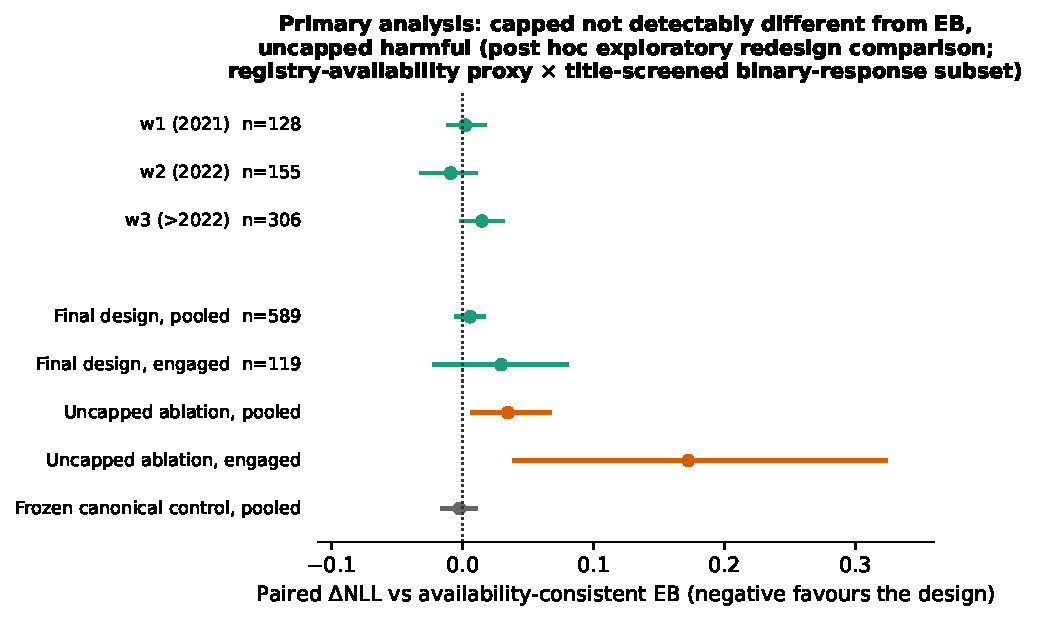
\includegraphics[width=0.92\textwidth]{F13_primary}
  \caption{\textbf{Primary analysis forest plot} (the capped-versus-uncapped
  contrast is a post hoc exploratory redesign comparison). Paired
  $\Delta$NLL versus
  the availability-consistent EB reference (negative favours the design)
  with bootstrap $95\%$ CIs, per window and pooled. The capped version
  (green) was neutral everywhere; the uncapped version (orange) was
  significantly harmful, concentrated in the engaged subgroup; the frozen
  canonical-model control (grey) is neutral, and the
  training-mechanism experiments of the text support attributing the
  uncapped harm to thin as-of-cutoff training pools.}
  \label{fig:primary}
\end{figure}

\paragraph{Availability-consistent detail.}
The non-strict full-corpus version of the availability analysis gives the
same picture and supplies its mechanics. Under
the analysis-time rule (everything an analyst could have used at each
cutoff: training queries and donors restricted to results posted by the
cutoff), the training pools shrink from $632/813/1{,}017$ to $323/494/651$
queries and the surviving donor observations to $27\%/36\%/45\%$; the EB
anchors are almost unchanged ($\mathrm{Beta}(0.68,1.66)$ at the final
cutoff). Retraining in this world and rescoring every forward query under
the per-query proxy rule is neutral (pooled $\Delta$ vs the
availability-consistent EB reference $-0.001$, CI $[-0.017,+0.016]$;
available-donor subgroup $-0.003$, CI $[-0.072,+0.072]$, $n=179$). The
upper-bound analyses of Sections~\ref{sec:headtohead-results}
and~\ref{sec:forward-results} measure what borrowing of registry-posted
results could contribute as availability matures; under the proxy they are
not yet realisable, and claims throughout the paper are scoped accordingly.

\subsection{Hypothetical upper bound I: EB-referenced held-out comparisons}
\label{sec:headtohead-results}
Table~\ref{tab:headtohead} reports every prior on the $20\%$ held-out split
($n = 281$; no method saw these outcomes during fitting) alongside the full
$1{,}407$-query development set (labelled: learned rows and EB fits include
their own training outcomes there), with design-time and outcome-adaptive
priors in separate blocks (Figure~\ref{fig:nll}).

Three comparisons carry the substance. First, \emph{the EB reference
reorders the field}: the two-parameter marginal prior (test NLL $2.9012$)
outperforms every borrowing construction except the learned ones ---
rule-weighted borrowing ($3.0542$; paired $\Delta$ vs EB $+0.153$, $95\%$ CI
$[+0.073,+0.237]$), the best-tuned robust-MAP ($3.0427$), and the classical
comparators all sit \emph{above} it. Much of what borrowing appeared to add
over the flat $\mathrm{Beta}(1,1)$ prior ($3.1641$) was marginal-distribution
information that a two-parameter fit supplies for free. Second, the
selective architecture supplies the only design-time priors below the EB
reference: the final design (capped) at
test NLL $2.8765$, paired $\Delta$ $-0.0247$ (CI $[-0.0588,+0.0097]$), and
its uncapped ablation at $2.8716$, $\Delta$ $-0.0295$
(CI $[-0.0722,+0.0109]$; $-0.0504$, CI $[-0.1066,+0.0003]$ against the
stratified EB variant)
--- consistent leads whose intervals narrowly include zero (stable across
five training seeds: $-0.029$ to $-0.038$ uncapped). Third, the
\emph{architecture matters, and the attribution is now exact}: against the
fixed-budget predecessor the
selective model improves by $-0.0581$ (CI $[-0.1170,-0.0026]$), a significant
paired gain, and the same holds out of time
(Section~\ref{sec:forward-results}). A full $2 \times 2$ factorial over the
two architectural changes (anchor: flat vs EB; total borrowing: fixed vs
learned) shows the gain is a genuine interaction rather than the sum of two
parts. On the pooled forward windows, relative to the intercept-EB reference:
flat anchor + fixed budget $+0.0399$; swapping only the anchor onto the
fixed-budget model erases the deficit but adds nothing ($+0.0002$); making
only the total borrowing learnable while keeping the flat anchor helps not at
all ($+0.0413$) --- a model free to withhold borrowing gains nothing when
withholding means falling back onto a flat prior far from the oncology
marginal; and only the combination is better than the reference ($-0.0266$).
Learnable total borrowing pays exactly when there is a sensible anchor to
fall back on. These results do not show that individual
historical candidates are expert-approved for borrowing.

\begin{table}[htbp]
\centering
\caption{EB-referenced borrowing head-to-head: mean beta-binomial predictive
NLL (lower is better) on the $20\%$ held-out split ($n=281$; the
\emph{principal upper-bound comparison} --- the primary analysis is
Table~\ref{tab:primary}) and on the full development set ($n=1{,}407$;
includes training
outcomes for learned rows and EB fits, reported for context). The final
design row is the capped selective prior; the uncapped selective row is
its ablation. Design-time
priors are fixed before the scored outcome; outcome-adaptive rows consult the
scored outcome through the SAM adapter, carry a partly mechanical advantage
(Section~\ref{sec:sam}), and are not compared as equals --- their proper
evaluation is the simulation of Section~\ref{sec:goldsim-results}.}
\label{tab:headtohead}
\small
\begin{tabular}{llrr}
\toprule
Method & Family & Test NLL ($n{=}281$) & Development NLL ($n{=}1{,}407$) \\
\midrule
\multicolumn{4}{l}{\emph{Design-time priors}}\\
\textbf{Final design (cap $0.5$)} & capped selective & \textbf{2.8765} & 2.8411 \\
selective (uncapped ablation) & learned, EB anchor & 2.8716 & 2.8335 \\
EB (intercept-only) & marginal reference & 2.9012 & 2.8992 \\
EB (disease-stratified) & marginal reference & 2.9221 & 2.8688 \\
two\_head (fixed budget) & learned ablation & 2.9297 & 2.8957 \\
fixed\_discount & rule & 3.0422 & 2.9916 \\
robust\_map ($w{=}0.5$) & robust-MAP & 3.0427 & 3.0019 \\
rule & rule & 3.0542 & 3.0100 \\
commensurate\_like & classical & 3.0900 & 3.0325 \\
weak\_only ($\mathrm{Beta}(1,1)$) & flat & 3.1641 & 3.1641 \\
robust\_map ($w{=}0.9$) & robust-MAP & 3.1978 & 3.0996 \\
map\_like & classical & 3.2687 & 3.2219 \\
power\_prior\_like & classical & 3.2807 & 3.2269 \\
\midrule
\multicolumn{4}{l}{\emph{Outcome-adaptive (not compared as equals; each SAM against its own weak component)}}\\
selective\_sam (anchored) & selective + SAM & 2.7995 & 2.7681 \\
two\_head\_sam & learned + SAM & 2.8154 & 2.7938 \\
rule\_sam & rule + SAM & 2.9226 & 2.9006 \\
\bottomrule
\end{tabular}
\end{table}

Point-prediction
metrics should be interpreted more cautiously than count-level predictive
likelihood: the current ORR point-prediction correlation was low, indicating
the model is better viewed as a borrowing-weight calibration model than as an
ORR regression model.

To answer whether a standard robust prior would suffice,
Table~\ref{tab:headtohead}
includes a tuned robust
meta-analytic-predictive (MAP) prior [5] in the style of the RBesT tools
[15]: its best-tuned configuration ($3.043$) beats flat-anchored borrowing
but not the plain EB reference, so the practical comparison is ``does any
candidate-level construction beat the marginal fit,'' and only the
selective architecture qualifies (tuning details in Supplement~S3).

\begin{figure}[htbp]
  \centering
  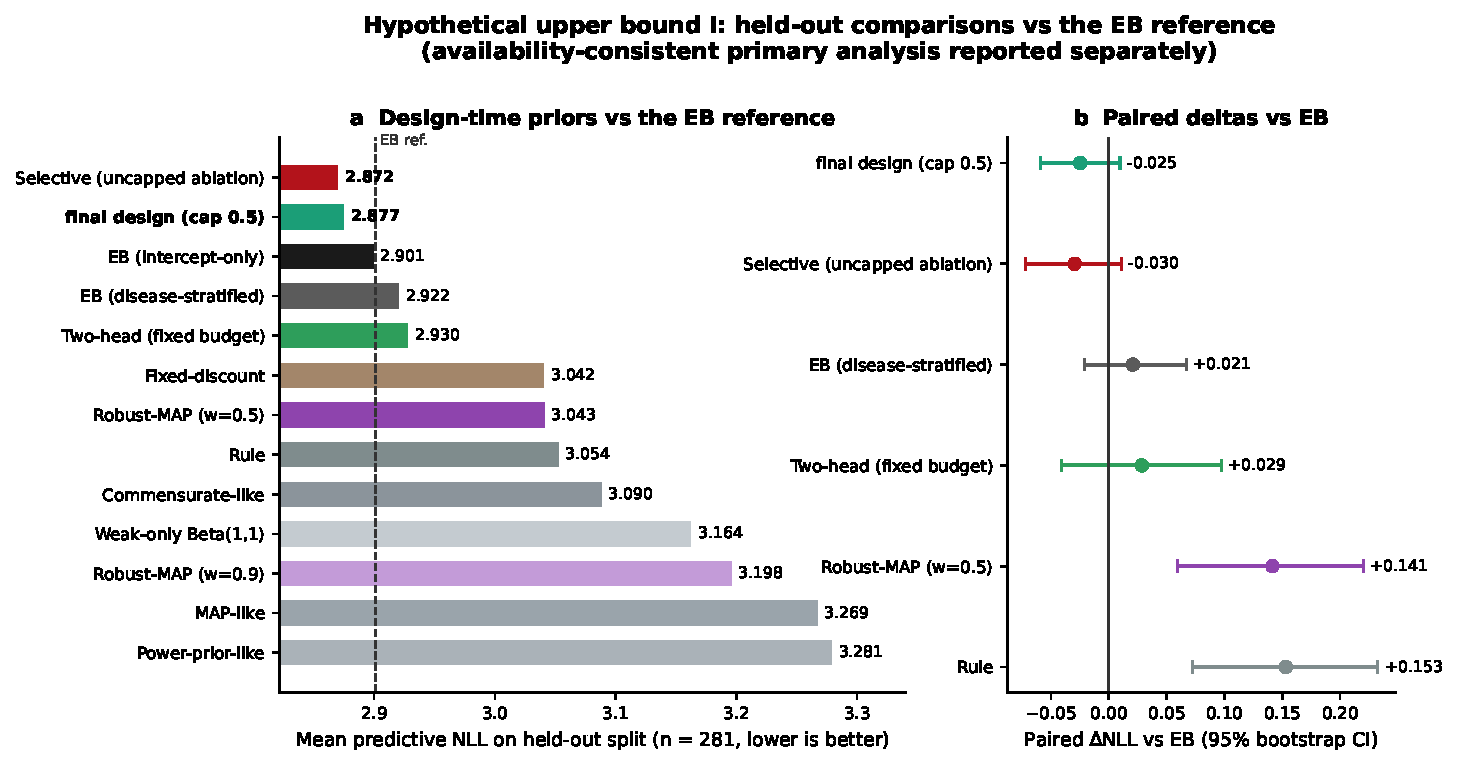
\includegraphics[width=\textwidth]{F1_headtohead_nll}
  \caption{\textbf{EB-referenced borrowing head-to-head (held-out split,
  $n=281$).} (a)~Design-time priors: mean beta-binomial predictive NLL (lower
  is better); the selective prior ($2.872$) is the only design-time prior
  below the intercept-only EB reference ($2.901$, dashed line), and the
  fixed-budget predecessor and all rule/classical/robust-MAP constructions sit
  above it. (b)~Paired deltas versus EB with bootstrap $95\%$ CIs for the
  learned priors and the strongest baselines.}
  \label{fig:nll}
\end{figure}

\subsection{Hypothetical upper bound II: forward validation on disjoint future windows (outcome-fit temporal split)}
\label{sec:forward-results}
To measure temporal generalization without leakage or double-counting, the
future was partitioned into disjoint windows by true primary completion date
--- $(2020\text{-}12\text{-}31, 2021\text{-}12\text{-}31]$ ($n=181$),
$(2021\text{-}12\text{-}31, 2022\text{-}12\text{-}31]$ ($n=204$), and
$>2022\text{-}12\text{-}31$ ($n=390$) --- and each window was scored exactly
once, by the selective model, fixed-budget ablation, and EB anchors refit
strictly on data completed on or before the window's left cutoff (past-only
training sets of $632$, $813$, and $1{,}017$ queries;
Figure~\ref{fig:forward}). Closed-form priors require no fitting and are
free of outcome and fitting leakage by construction; the split alone does not
enforce donor-level availability at decision time (a donor completed before
a cutoff may have posted results later), so we label it an outcome-fit
temporal split without donor-availability control rather than leakage-free.
Outcome-adaptive SAM rows are excluded here by
the partition rule of Section~\ref{sec:eval}. Everything in this subsection
treats all posted results as available and is reported as an upper bound on
what borrowing of registry results \emph{could} contribute as availability
matures; none of it carries decision-time evidential weight
(the availability-consistent primary analysis is
Section~\ref{sec:primary-results}).

Pooled over the $775$ future trials (Table~\ref{tab:forward}), the final
design (capped) achieved NLL $2.8027$ versus $2.8440$ for the past-fit EB
reference (paired $\Delta$ $-0.0413$, $95\%$ CI $[-0.0625,-0.0202]$); its
uncapped ablation reached $2.8175$
($\Delta$ $-0.0266$, CI $[-0.0591,+0.0064]$) and $2.8839$ for
the fixed-budget predecessor ($\Delta$ $-0.0665$, CI $[-0.0993,-0.0346]$ ---
the architectural gain replicates out of time). Per window, the selective
lead over EB was $-0.0062$ (CI $[-0.0874,+0.0855]$), $-0.0074$
($[-0.0704,+0.0565]$), and $-0.0461$ ($[-0.0861,-0.0083]$): significant only
in the most recent window. Because the three windows are examined together,
per-window significance should be judged under multiplicity control
(Bonferroni over three windows, $98.33\%$ intervals), and because ``the
window whose model saw the most training data'' could be confounded with
window composition, we ran the controlled experiment: all three fold models
scored on the \emph{same} $390$ window-3 queries, so that training-pool size
($632/813/1{,}017$) varies with composition fixed. The models improved in
that order --- deltas versus EB of $-0.0255$, $-0.0225$, and $-0.0461$, with
the $1{,}017$-example model beating the $813$-example model on the same
queries by $-0.0236$ (CI $[-0.0424,-0.0057]$) --- so the learning-curve
reading survives the composition control, though window-3 queries may still
differ in other ways. In the pre-specified
information-rich subgroup ($I \ge 8$; $n=291$) the selective lead over EB was
$-0.0585$ (CI $[-0.1240,+0.0127]$, win rate $60\%$), against $-0.0074$
(CI $[-0.0381,+0.0223]$) in the information-poor remainder --- directionally
as pre-specified, though the subgroup interval includes zero. The
disease-stratified EB reference performed strongly here ($2.8152$; $\Delta$ vs
intercept EB $-0.0288$, CI $[-0.0452,-0.0128]$) and was statistically
indistinguishable from the selective prior pooled over windows ($\Delta$
$+0.0022$, CI $[-0.0281,+0.0345]$), though unstable across settings (it was
\emph{worse} than intercept EB on the test split, $+0.0209$).

\paragraph{Stability across seeds and the pre-registered ensemble.} All
single-fit results above use one training seed, so we retrained every fit
under four additional seeds and evaluated the seed-averaged mixture prior.
The ensembling step was written down in advance, within this revision, as the
one remaining mechanical lever, to be reported whichever way it came out;
because that pre-specification is internal to the revision cycle rather than
an independent prospective registration, we label every ensemble result
\emph{exploratory}. The architectural
gain is stable (pooled forward delta versus the fixed-budget predecessor
between $-0.058$ and $-0.075$ across seeds), the triage policy is stable
(borrowed-mass quartiles within $0.15$--$0.21 / 0.36$--$0.47 / 0.62$--$0.73$),
and the selective-versus-EB delta is negative under every seed (pooled
forward $-0.018$ to $-0.035$; test $-0.029$ to $-0.038$), with single-seed
intervals crossing zero for four of five seeds. The five-seed ensemble prior
performs better than the typical single seed: pooled forward NLL $2.8084$
versus $2.8440$ for EB ($\Delta$ $-0.0356$, CI $[-0.0670,-0.0059]$ --- the
single pre-specified aggregate test, now excluding zero, but exploratory in
the sense above and confined to the upper-bound tier), $-0.0755$
(CI $[-0.1051,-0.0442]$) versus the fixed-budget predecessor, and a window-3
delta of $-0.0480$ whose Bonferroni-adjusted $98.33\%$ interval
$[-0.0947,-0.0024]$ still excludes zero; the ensemble's test-split delta
($-0.0336$, CI $[-0.0755,+0.0070]$) remains inconclusive. We report the
single-seed analysis first because it was specified first, and the ensemble
as the exploratory upgrade; both live entirely in the upper-bound tier and
neither carries decision-time evidential weight. Marginal
references remain, in short, hard to beat: the selective model's demonstrated
advantages over them are the significant most-recent-window win (which
survives multiplicity adjustment under the exploratory ensemble), the
ensemble's aggregate lead, the
significant architectural improvement, and the triage behaviour
of Section~\ref{sec:triage-results}, not an across-the-board dominance ---
and none of it survives the registry-availability proxy of the primary
analysis above. Restricting this upper-bound tier to the title-screened binary-response
subset preserves the pattern for the uncapped prior (retrained
title-screened pooled $\Delta$ $-0.034$, CI $[-0.074,+0.007]$; frozen-model
title-screened filtering $-0.033$, CI $[-0.068,+0.001]$) --- so the
direction of the advantage does not depend on the unscreened endpoint mix,
though because the screened subset itself retains $\approx 20\%$ non-ORR
endpoints (Section~\ref{sec:eval}), none of these results should be read
as established for a pure-ORR population.

\begin{figure}[htbp]
  \centering
  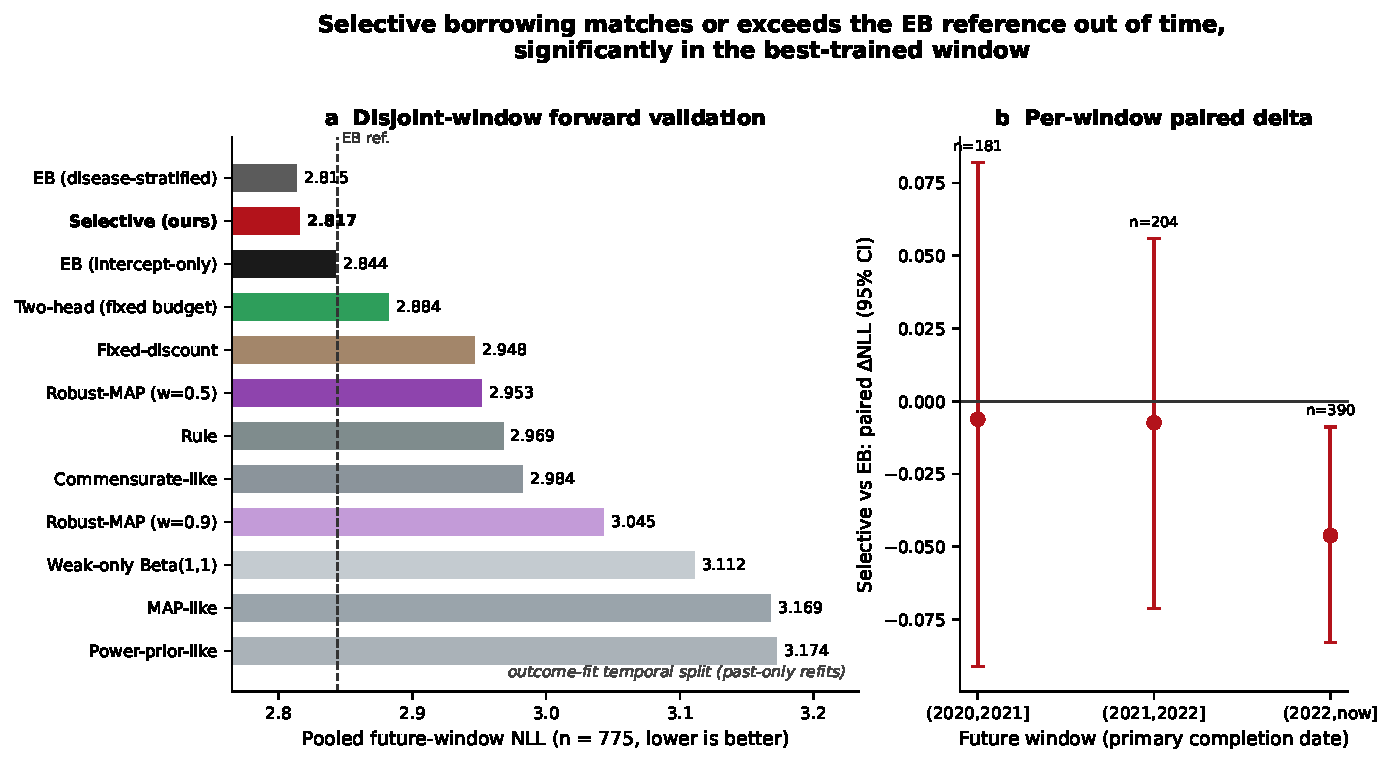
\includegraphics[width=\textwidth]{F2_forward_validation}
  \caption{\textbf{Forward validation on disjoint future
  windows (hypothetical full-information upper bound; the
  availability-consistent primary analysis shows no benefit).} (a)~NLL
  pooled over the three disjoint windows ($n=775$) for
  design-time priors; the selective prior ($2.818$) and the disease-stratified
  EB reference ($2.815$) lead, the intercept EB reference is at $2.844$
  (dashed line), and the fixed-budget predecessor trails at $2.884$.
  (b)~Per-window paired delta of the selective prior versus intercept EB with
  bootstrap $95\%$ CIs; the most recent, best-trained window is significant
  ($-0.046$, CI $[-0.086,-0.008]$).}
  \label{fig:forward}
\end{figure}

\begin{table}[htbp]
\centering
\caption{Forward validation on disjoint future windows --- hypothetical
full-information upper bound (outcome-fit temporal split with past-only
refits; donor availability at decision time NOT enforced; see the primary
analysis of Section~\ref{sec:primary-results} for the availability-consistent
result, which shows no benefit). NLL pooled over the three windows
($n=775$); paired delta versus the past-fit intercept-EB reference with
bootstrap $95\%$ CI. The final design row is the capped selective prior
(cap applied at scoring); the uncapped selective row is its ablation; the
ensemble row is exploratory. Learned rows and EB
anchors are refit on past-only data at each window's left cutoff.}
\label{tab:forward}
\begin{tabular}{lrl}
\toprule
Method & Pooled future NLL & Paired $\Delta$ vs EB [$95\%$ CI] \\
\midrule
\textbf{Final design (cap $0.5$)} & \textbf{2.8027} &
$\mathbf{-0.0413}$ $[-0.0625,-0.0202]$ \\
selective (5-seed ensemble) & 2.8084 & $-0.0356$ $[-0.0670,-0.0059]$ \\
EB (disease-stratified) & 2.8152 & $-0.0288$ $[-0.0452,-0.0128]$ \\
selective (uncapped ablation) & 2.8175 & $-0.0266$ $[-0.0591,+0.0064]$ \\
EB (intercept-only) & 2.8440 & reference \\
two\_head (fixed budget) & 2.8839 & $+0.0399$ $[-0.0071,+0.0872]$ \\
fixed\_discount & 2.9483 & --- \\
robust\_map ($w{=}0.5$) & 2.9535 & --- \\
rule & 2.9694 & --- \\
commensurate\_like & 2.9841 & --- \\
robust\_map ($w{=}0.9$) & 3.0445 & --- \\
weak\_only ($\mathrm{Beta}(1,1)$) & 3.1122 & --- \\
map\_like & 3.1693 & --- \\
power\_prior\_like & 3.1737 & --- \\
\bottomrule
\end{tabular}
\end{table}

\paragraph{The final design on the upper-bound tiers.} Scoring the same
tiers with the mixture-mass cap of the final design
(Section~\ref{sec:cap}; the cap was fixed at $0.5$ in the previous revision,
before any of these numbers were computed) \emph{improves} the upper-bound
results rather than taxing them: pooled forward $\Delta$ versus EB
$-0.0413$ (CI $[-0.0625,-0.0202]$ --- significant, where the uncapped prior's
$-0.0266$ was not), held-out test $-0.0247$ (CI $[-0.0588,+0.0097]$),
retrained title-screened subset $-0.0485$ (CI $[-0.0742,-0.0233]$), and
frozen-model title-screened filtering $-0.0440$ (CI $[-0.0667,-0.0223]$);
neighbouring caps $0.3$ and $0.7$ give the same picture (forward $-0.0365$
and $-0.0380$, both significant), and the intervals survive strongest-donor
block resampling (forward $[-0.0665,-0.0166]$, $365$ blocks;
retrained title-screened $[-0.0815,-0.0189]$ and frozen $[-0.0707,-0.0179]$,
$267$ blocks each). The block rule here --- strongest gated donor by rule
weight, with no-donor queries as singleton blocks --- differs in its
handling of no-donor queries from the earlier released dependence
analysis ($346$ blocks over the same $775$ forward queries), which is why
the counts differ; the forward interval is insensitive to the rule
(strongest-by-rule-weight $[-0.067,-0.017]$; no-donor queries pooled
$[-0.067,-0.018]$; strongest-by-gate $[-0.063,-0.020]$; Supplement~S2). Restricting historical mass evidently acts
as regularisation against over-confident allocations out of time, so the
harm-attenuating mechanism costs nothing on the favourable tiers. One
scoping label governs all of these numbers: the cap was added
\emph{after} the uncapped held-out and forward results of earlier
revisions had been examined, and re-applying it to those same outcome sets
cannot restore a lockbox --- every capped real-data result in this paper
is therefore a \emph{post hoc exploratory redesign evaluation}, not
independent confirmation, which would require a new registry vintage, an
untouched time window, or external data. Within that label, the two
significant title-screened upper-bound intervals are the strongest
real-data evidence for the final design; they remain upper-bound-tier
evidence, and they inherit the title-screened subset's measured
$\approx 80\%$ strict-ORR purity, so they are statements about the
screened binary-response estimand, not about a pure ORR population.

\paragraph{Dependence and unit-provenance sensitivity.} Queries are distinct
registered trials but share donors ($12.7\%$ of forward query pairs share at
least one gated donor), so we recomputed the headline intervals under a
donor-block bootstrap (blocks defined by each query's strongest gated
donor; $346$ blocks, largest $36$): the architectural gain and the
window-3 delta survive (intervals $[-0.105,-0.030]$ and
$[-0.089,-0.007]$), while the pooled
selective-versus-EB interval remains zero-crossing ($[-0.062,+0.008]$),
essentially as under query-level resampling; leaving out all queries touching
any one of the ten most-shared donors moves the pooled delta between
$-0.018$ and $-0.037$. These block schemes are \emph{approximate}
dependence adjustments, not exact ones: the sharing graph is so connected
that coarser blockings degenerate (connected components put $98\%$ of
queries in one block; unioning each query's top-two donors already yields a
block holding $89\%$, whose resampled interval, $[-0.139,-0.017]$, we show
for transparency but regard as unstable rather than evidential), so
residual cross-block correlation through secondary shared donors remains
possible and none of these intervals should be read as fully
dependence-adjusted. Separately, because $54\%$ of donor observations and
$49\%$ of query outcomes are reconstructed from percentage-reported values,
we re-ran the comparison keeping only count-reported data: restricted to
count-reported query outcomes the pooled delta is $-0.003$
(CI $[-0.049,+0.047]$, $n=380$), and dropping percentage-derived donor
observations from the priors gives $-0.001$ (CI $[-0.022,+0.020]$). The
aggregate advantage therefore concentrates in percentage-derived,
predominantly recent, larger trials (their pooled delta $-0.050$, median
year 2023) --- consistent with the availability gradient above. The completed single-rater audit
(Section~6.1) specifically vindicates the percentage-reconstruction path
($42/42$ denominator agreement in that stratum) and shows the headline
comparisons are insensitive to every numeric error it found (shifts under
$0.001$ NLL).
\label{sec:calib-results}
We assessed calibration against the real held-out outcome on the held-out test
split using the randomized probability integral transform (PIT) and the
empirical coverage of equal-tailed \emph{prediction} intervals for the
observed count $y_0$ --- these are prior-predictive intervals for the outcome,
not credible intervals for the latent rate $\theta$
(Figure~\ref{fig:calib}, Table~\ref{tab:calib}). Because the predictive
distribution is discrete, an equal-tailed interval from a \emph{correctly
specified} predictive attains at least its nominal level; empirically the
well-specified methods do over-cover, while the optimistic flat-anchored and
classical priors under-cover despite the discreteness (Table~\ref{tab:calib}:
e.g.\ $0.384$ and $0.936$ at nominal $0.50$ and $0.95$), and we characterize
coverage precisely rather than calling it nominal. The
intercept-only EB reference is, unsurprisingly, the best-calibrated
distribution for the marginal outcome (PIT KS $0.035$). The selective prior
comes closest to it among borrowing methods (KS $0.094$; coverage
$0.683/0.925/0.975$ at nominal $0.50/0.80/0.95$ --- conservative at $50\%$,
partly by discreteness) while achieving lower NLL, whereas the fixed-budget
predecessor (KS $0.173$), rule ($0.252$), and the flat-anchored and classical
priors (KS $0.32$--$0.35$) are systematically optimistic --- the weak-only
prior's $50\%$ intervals covered only $0.46$, and map- and power-prior-like
constructions under-covered even at $95\%$ ($0.947$ and $0.936$). The
selectivity mechanism thus improves calibration and NLL together, rather than
trading one for the other.

\begin{table}[htbp]
\centering
\caption{Predictive calibration diagnostics on the held-out split
($n=281$): PIT Kolmogorov--Smirnov distance to uniformity (smaller is better)
and empirical coverage of equal-tailed $50/80/95\%$ \emph{prediction}
intervals for the observed count (discreteness makes these conservative when
the predictive law is well specified; misspecified priors can and do
under-cover). Design-time and outcome-adaptive blocks as in
Table~\ref{tab:headtohead}. The selective prior approaches the calibration of
the EB reference while achieving lower NLL; flat-anchored and classical priors
are systematically optimistic.}
\label{tab:calib}
\begin{tabular}{lrrrrr}
\toprule
Method & Mean NLL & PIT KS & Cov50 & Cov80 & Cov95 \\
\midrule
\multicolumn{6}{l}{\emph{Design-time priors}}\\
EB (intercept-only) & 2.901 & \textbf{0.035} & 0.680 & 0.911 & 0.979 \\
\textbf{Final design (cap $0.5$)} & \textbf{2.877} & 0.097 & 0.690 & 0.929 & 0.979 \\
selective (uncapped ablation) & 2.872 & 0.094 & 0.683 & 0.925 & 0.975 \\
two\_head (fixed budget) & 2.930 & 0.173 & 0.544 & 0.858 & 0.972 \\
rule & 3.054 & 0.252 & 0.484 & 0.819 & 0.979 \\
weak\_only ($\mathrm{Beta}(1,1)$) & 3.164 & 0.317 & 0.459 & 0.819 & 0.996 \\
map\_like & 3.269 & 0.324 & 0.384 & 0.694 & 0.947 \\
power\_prior\_like & 3.281 & 0.315 & 0.395 & 0.676 & 0.936 \\
\midrule
\multicolumn{6}{l}{\emph{Outcome-adaptive (labelled; not compared as equals)}}\\
selective\_sam (anchored) & 2.800 & 0.094 & 0.708 & 0.932 & 0.982 \\
two\_head\_sam & 2.815 & 0.187 & 0.598 & 0.911 & 0.996 \\
rule\_sam & 2.923 & 0.259 & 0.537 & 0.883 & 0.996 \\
\bottomrule
\end{tabular}
\end{table}

\begin{figure}[htbp]
  \centering
  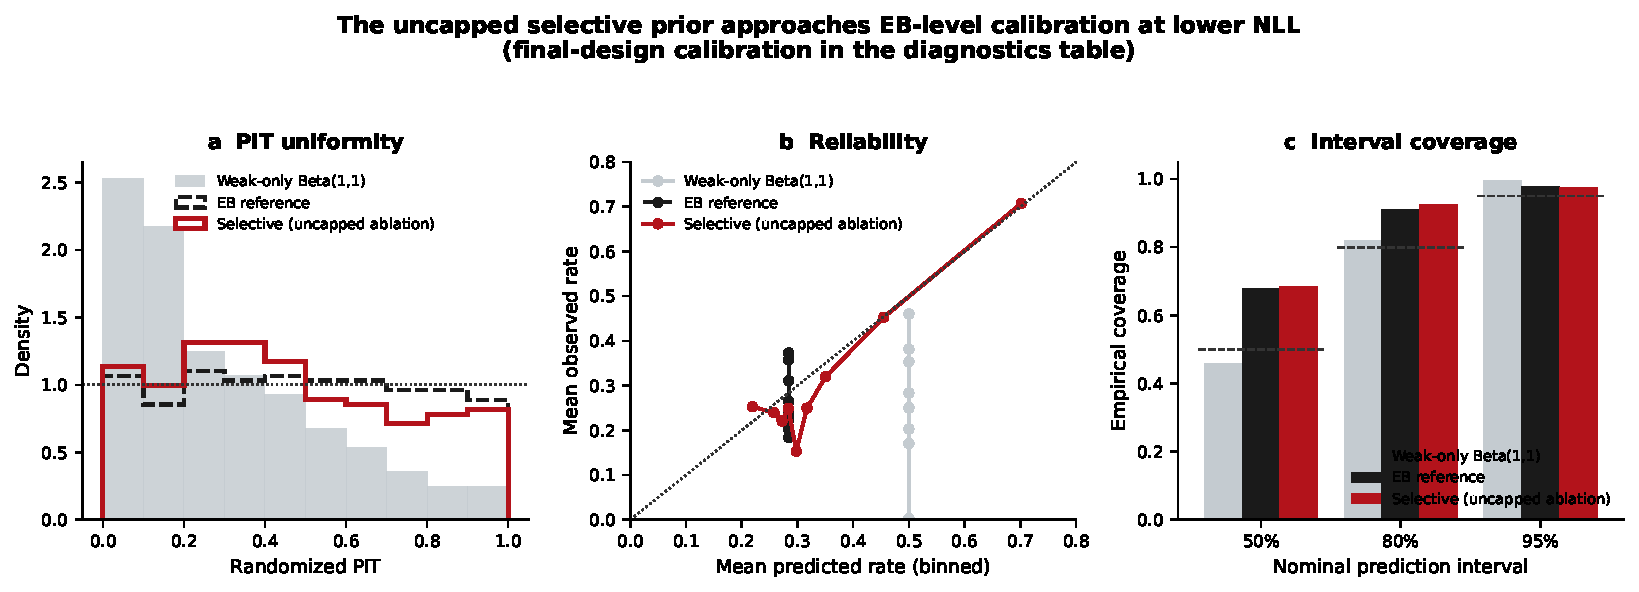
\includegraphics[width=\textwidth]{F3_calibration}
  \caption{\textbf{Predictive calibration (held-out split).} (a)~PIT
  uniformity, (b)~reliability curve (predicted vs.\ observed response rate),
  and (c)~$50/80/95\%$ prediction-interval coverage, comparing the selective
  prior against the intercept-only EB reference and the weak-only prior
  (the fixed-budget predecessor and remaining methods appear in
  Table~\ref{tab:calib}). The selective prior approaches the EB
  reference's PIT uniformity (KS $0.094$ vs $0.035$) at lower NLL, while
  flat-anchored priors are systematically optimistic; the well-specified
  methods over-cover (equal-tailed intervals on a discrete predictive are
  conservative when the predictive law is right), whereas the optimistic
  priors under-cover despite that discreteness.}
  \label{fig:calib}
\end{figure}

\subsection{The learned total borrowing behaves as design-time triage}
\label{sec:triage-results}
The selectivity mechanism is directly inspectable, because the learned
$1-\lamz$ is a number per query. Over the pooled forward windows the borrowed
mass spanned its range (quartiles $0.15/0.36/0.65$) rather than sitting at a
forced constant (the fixed-budget predecessor allocates $\approx 0.79$
whenever any candidate passes its gate), and it tracked the pre-specified
design-time information measure (Spearman $+0.59$ with $I$;
Figure~\ref{fig:triage}). That correlation alone, however, shows only that
the network uses the candidate-information content of its own inputs, so we
test the claim that matters: does the learned mass rank the \emph{realized}
benefit of borrowing on unseen data? Taking per-query benefit as
$\mathrm{NLL}_{\mathrm{EB}} - \mathrm{NLL}_{\mathrm{selective}}$ over the
pooled forward windows, the rank correlation between learned mass and
realized benefit is $+0.16$ (bootstrap CI $[+0.08, +0.24]$) --- modest, but
stable at $+0.16$ in each of the three windows separately, and slightly
better than the hand rule's information measure achieves ($+0.14$).
Where the realized value concentrates is more informative than the
correlation: in the lowest mass tertile (mean mass $0.10$) the selective
prior is exactly neutral against EB ($+0.003$, CI $[-0.007,+0.012]$) where
the fixed-budget predecessor was being badly hurt ($+0.148$ against EB on the
same queries) --- withholding eliminates the forced-borrowing damage --- and
the middle tertile carries a significant win ($-0.054$, CI
$[-0.089,-0.019]$), while the highest tertile is directionally favourable
but noisy ($-0.029$, CI $[-0.117,+0.060]$). Selecting the same number of
queries by top learned mass as the pre-specified $I \ge 8$ rule selects
yields a comparable mean benefit ($+0.035$ versus $+0.058$, both CIs
crossing zero), so the learned triage matches, but does not beat, the hand
rule as a selection device. The model learned, from features alone, the
triage that the subgroup analysis of Section~\ref{sec:forward-results}
imposed by hand --- and its demonstrated value is harm avoidance where
information is thin, more than superiority where information is rich.

\begin{figure}[htbp]
  \centering
  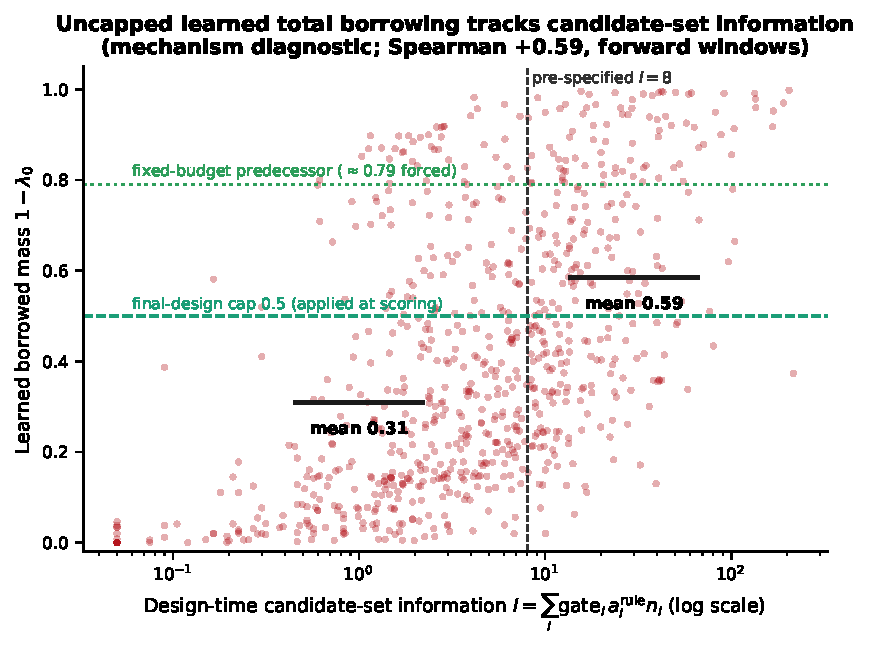
\includegraphics[width=0.72\textwidth]{F12_triage}
  \caption{\textbf{Learned borrowing triage.} Learned borrowed mass
  $1-\lambda_0$ against the pre-specified design-time candidate-set
  information measure $I$ (log scale), one point per forward-window query.
  Mean borrowed mass is $0.31$ below the pre-specified threshold $I=8$ and
  $0.59$ above it (Spearman $+0.59$); the fixed-budget predecessor forces
  $\approx 0.79$ everywhere (dotted line).}
  \label{fig:triage}
\end{figure}

A mechanism check --- diagnostic only, because it conditions on the scored
outcome and can never be a selection rule --- explains why triage is the right
policy: among forward queries whose retrieved donors' consensus rate landed
within $0.15$ of the eventual observed rate, candidate borrowing beat the EB
reference decisively (paired deltas $-0.25$ to $-0.32$, win rates
$82$--$84\%$), whereas for the majority of queries whose donor consensus was
farther away, indiscriminate borrowing hurt ($+0.22$). Candidate-level
borrowing works precisely when the retrieved candidates are genuinely
informative about the query; the selective architecture's contribution is to
predict, before the outcome exists, how much that is likely to be true.

\subsection{Gold-standard simulation: operating characteristics}
\label{sec:goldsim-results}

We now report the simulation set up in Section~\ref{sec:simulation}. The
data-generating mechanism produced the intended structure. Across the five
estimation scenarios, between $8\%$ and $43\%$ of donors were genuinely
exchangeable, trap donors (surface-similar but not exchangeable) accounted for
$19\%$ to $66\%$, and hidden gems for $2\%$ to $15\%$, from $24{,}000$ candidates
per scenario. Surface similarity and borrowability were thus substantially
decoupled by construction, which is the property the simulation exists to test.

Table~\ref{tab:design-oc} reports the design-based operating characteristics,
now including the selective architecture. Three findings matter, and they cut
in different directions.

First, under exchangeability the selective prior converts its predictive
gains into design gains. With no prior-data conflict its \emph{estimated}
type I error was
$0.024$ (nominal $0.025$; no-borrowing reference $0.037$; $2{,}000$
replicates, so this is a point estimate compatible with modest inflation,
not demonstrated control) with power $0.613$
--- the highest observed power among methods whose estimated error was
$\le 0.025$ in that cell, against $0.588$
for the fixed-budget predecessor, $0.556$ for the rule mixture, and $0.536$
without borrowing. The EB-only reference is safe but pays for its ignorance of
the candidates (power $0.497$); full pooling and the power prior remain
unusable ($0.584$ and $0.484$ type I error at zero conflict).

Second --- and this is the central safety finding of the revision --- the
learnable total borrowing \emph{removes the cap} that the fixed budget had
accidentally provided. Under uniform whole-set conflict the standalone
selective prior's type I error rises steeply: $0.056$, $0.145$, and $0.243$ at
logit shifts of $0.5$, $1.0$, and $1.5$, versus $0.072$ and $0.061$ at shifts
$1.0$ and $1.5$ for the fixed-budget predecessor, $0.050$ for the rule, and
$0.047$ for robust-MAP. The mechanism is exactly the one predicted by the
unidentifiability argument of Section~6.2: a uniformly displaced donor set
looks internally consistent and information-rich at design time, so a model
free to raise its total borrowing does so --- the same behaviour that earns
power under exchangeability ($0.766$ at shift $1.0$ in the alternative world,
partly borrowed bias) inflates the null rejection rate when the displacement
is real. The fixed-discount ablation ($0.079$ at shift $1.0$) shows most of
the inflation enters through the total-borrowing head rather than the
discount head.

Third, the anchored SAM adapter mitigates --- but does not eliminate --- the
inflation while keeping the
no-conflict benefit: selective + SAM held type I error to $0.029/0.041/0.070/
0.046$ across the conflict grid --- comparable to the fixed-budget + SAM
variant, but still $2.8\times$ nominal at shift $1.0$ --- with power $0.594$
at zero conflict, still above every
non-selective controlled method. The structural lesson stands ---
the selectivity that makes the prior efficient when
borrowing is warranted is precisely what makes it exploitable by conflict
that design-time features cannot see, so the uncapped prior must never be
deployed bare --- but the component that discharges this obligation in the
final design is the mixture-mass cap, not SAM: the cap achieves a
tighter worst case ($0.044$ versus SAM's $0.070$) without consuming the
outcome, and adding SAM on top of the cap is measurably redundant. What
either mechanism provides is mitigation, not strict control, and we
quantify that distinction next.

\paragraph{Calibrated designs: the impossibility premise, the cap curve,
and the mixture frame.} A complete design must be judged with its
calibrated threshold, and the calibration frame decides what can be won.
The grid is two-dimensional and now two-sided: uniform shifts $-1.5$ to
$+1.5$ at full conflict \emph{and} partial-conflict cells in which only a
fraction $f \in \{0.25, 0.5, 0.75\}$ of donors is displaced (partial
conflict creates within-set heterogeneity and is easier: the standalone
selective prior's worst partial-conflict cell reaches $0.112$, versus
$0.243$ under uniform displacement); per-replicate posterior probabilities
are stored, so every design's rejection rate is available at any threshold.
Three layers of findings follow.

\emph{First, the worst-case frame concedes everything in this setting, for
every borrowing method, ours included.} Empirical-quantile worst-case
calibration (the $97.5\%$ quantile over all null cells; a Monte Carlo
estimate, not an exact threshold) yields $\hat\tau^{*} = 0.9999$ for the
standalone selective prior --- control is technically reachable but
degenerate, with no-conflict power $0.069$ against the no-borrowing
reference's $0.448$ at its own $\hat\tau^{*}$ --- and for every other design
a $\hat\tau^{*}$ at which no material power advantage over no borrowing
survives (the largest apparent gain, $+0.7$ points at cap $0.1$, is within
Monte Carlo error). This is the expected outcome for a one-parameter,
one-sided design of the present kind, where [28]'s conditions apply; we do
not claim the impossibility for settings outside that scope. We therefore
report $\hat\tau^{*}$ for completeness and turn to the corpus-specific
decision analysis of Section~\ref{sec:goldsim}, labelled exploratory.

\emph{Second, the cap--power--error curve} (Table~\ref{tab:capcurve})
answers what the previously fixed cap value trades away. Along
$c \in \{0.1,\dots,0.9\}$, uncalibrated worst-case type~I error rises
monotonically from $0.033$ to $0.070$ (uncapped: $0.243$); mixture power at
the mixture-calibrated threshold is flat at $0.519$--$0.521$ for
$c \le 0.5$ and decays beyond; caps above $0.7$ violate the pre-specified
$0.05$ worst-case ceiling. What distinguishes caps below the flat top is
the \emph{shape} of the power profile: at $c = 0.1$ the design hugs the
references everywhere (favourable-band gain $+1$--$2$ points), while at
the previously fixed $c = 0.5$ the gain where donors are approximately
exchangeable reaches $+5$ points at the same mixture average --- the cap
buys conditional upside with attenuated downside rather than
mixture-average performance. We retain $c = 0.5$ as fixed before any of the round-4 cap
analyses (Section~\ref{sec:cap}) rather than re-tuning on this curve; SAM added to
any capped design changes worst cases by at most $0.004$ while costing
$1$--$2$ points of mixture power (e.g.\ cap $0.5$: $0.5104$ with SAM versus
$0.5210$ without), which is the measured redundancy behind its exclusion
from the final design.

\begin{table}[htbp]
\centering
\small
\caption{Cap--power--error curve on the selection batch ($2{,}000$
replicates per cell; two-sided uniform plus partial-conflict null cells).
$\hat\tau^{*}$: empirical-quantile worst-case threshold (worst null cell
$\le 0.025$), with no-conflict power at $\hat\tau^{*}$.
$\tau_{\mathrm{mix}}$: mixture-calibrated
threshold (drift-weighted average type~I $\le 0.025$), with mixture power
and worst-case type~I at $\tau_{\mathrm{mix}}$; the pre-specified tolerated
pointwise inflation ceiling
for the latter is $0.05$. The final design row is bold; SAM variants shown
for the redundancy measurement.}
\label{tab:capcurve}
\begin{tabular}{lcccccc}
\hline
 & Worst T1 & \multicolumn{2}{c}{Worst-case frame} &
\multicolumn{3}{c}{Mixture frame} \\
Design & @$0.975$ & $\hat\tau^{*}$ & Power$_{s=0}$ & $\tau_{\mathrm{mix}}$ &
Mix.\ power & Worst T1 \\
\hline
No borrowing         & 0.038 & 0.9857 & 0.448 & 0.9805 & 0.511 & 0.032 \\
EB-only reference    & 0.032 & 0.9820 & 0.448 & 0.9750 & 0.516 & 0.032 \\
Selective, cap $0.1$ & 0.033 & 0.9828 & 0.455 & 0.9750 & 0.521 & 0.033 \\
Selective, cap $0.2$ & 0.036 & 0.9840 & 0.453 & 0.9750 & 0.521 & 0.036 \\
Selective, cap $0.3$ & 0.038 & 0.9856 & 0.439 & 0.9755 & 0.519 & 0.038 \\
Selective, cap $0.4$ & 0.042 & 0.9866 & 0.437 & 0.9755 & 0.519 & 0.041 \\
\textbf{Selective, cap $0.5$ (final design)}
                     & 0.044 & 0.9876 & 0.432 & 0.9755 & \textbf{0.521} & 0.044 \\
Selective, cap $0.6$ & 0.047 & 0.9881 & 0.438 & 0.9765 & 0.515 & 0.045 \\
Selective, cap $0.7$ & 0.052 & 0.9903 & 0.418 & 0.9780 & 0.509 & 0.050 \\
Selective, cap $0.8$ & 0.060 & 0.9915 & 0.409 & 0.9795 & 0.502 & 0.052$^{\dagger}$ \\
Selective, cap $0.9$ & 0.070 & 0.9935 & 0.392 & 0.9825 & 0.489 & 0.057$^{\dagger}$ \\
Selective (uncapped) & 0.243 & 0.9999 & 0.069 & 0.9980 & 0.343 & 0.093$^{\dagger}$ \\
Selective + SAM      & 0.070 & 0.9944 & 0.391 & 0.9840 & 0.483 & 0.058$^{\dagger}$ \\
Cap $0.5$ + SAM      & 0.044 & 0.9875 & 0.435 & 0.9780 & 0.510 & 0.040 \\
Rule + SAM           & 0.050 & 0.9891 & 0.430 & 0.9790 & 0.518 & 0.044 \\
Two-head + pro.\ + SAM & 0.070 & 0.9923 & 0.417 & 0.9835 & 0.495 & 0.051$^{\dagger}$ \\
\hline
\multicolumn{7}{l}{\footnotesize $^{\dagger}$ exceeds the pre-specified
$0.05$ worst-case ceiling at $\tau_{\mathrm{mix}}$; ineligible as a final
design.}\\
\end{tabular}
\end{table}

\emph{Third, the corpus-specific decision analysis (exploratory) finds at
most a marginal size-matched average gain, with the conditional structure
as the substantive content} (Figure~\ref{fig:profiles};
Tables~\ref{tab:calibrated} and~\ref{tab:sizematched}). At the frozen
thresholds, on the independent $10{,}000$-replicate batch, the final
design's drift-weighted average type~I error is $0.0258$ (Monte Carlo se
$0.0005$) against calibrated no borrowing's $0.0251$ --- so the frozen
thresholds do \emph{not} deliver a point estimate $\le 0.025$, and the two
designs are not at exactly the same size; both facts matter. Its worst
null cell is $0.0360$ (Clopper--Pearson $95\%$ upper bound $0.0392$;
Bonferroni over all $22$ null cells, $0.0416$ --- inside the tolerated
pointwise inflation ceiling of $0.05$, which is to say: tolerated, not
controlled at nominal). At those unequal sizes the mixture-power
difference is $+0.0066$. Because a $0.0007$ size difference can buy power,
we re-read the same validation data with thresholds adjusted to equal
size --- an \emph{in-validation size-adjusted reanalysis}, distinct from
the frozen-threshold validation above, since the adjusted thresholds are
estimated on the validation batch itself. Single analyses give positive
point estimates: full-batch interpolation (thresholds so every design's
average type~I equals no-borrowing's $0.0251$) gives $+0.0024$
(within-replicate MC se $0.0007$) for the final design, $+0.0057$ for cap
$0.3$, $-0.0015$ for the EB anchor alone (its apparent gain was entirely
liberality), $-0.0010$ for cap $0.5$ + SAM; a single two-fold cross-fit
(thresholds from one half of each cell, evaluation on the other) gives
$+0.0057$ for the final design. But \emph{repeating} the cross-fit under
$200$ random half-splits --- so that threshold-estimation and split
variability actually propagate --- centres the final design's
size-adjusted difference at $-0.0007$ (split SD $0.0011$; $95\%$ split
interval $[-0.0014, +0.0039]$; only $4\%$ of splits positive). The
positive single-analysis point estimates are therefore within
threshold-estimation noise, and we conclude that \emph{no average net
power difference at matched size has been established in either
direction}; mixing-measure estimation error and the deconvolution's
normal form sit unpropagated on top of even this. Under a conservative
calibration requiring the Monte Carlo $95\%$ upper bound of average
type~I to sit below $0.025$ (the \emph{smallest} threshold satisfying the
constraint, since power falls in the threshold), the single-analysis
ordering is unchanged (no borrowing
$0.5028$; final design $0.5055$; cap $0.3$ $0.5090$) and carries the same
caveat. The size-matched
single-analysis point estimates are positive under every corpus-derived
mixing measure examined
(Table~\ref{tab:sizematched}: $+0.0010$ to $+0.0063$; weight bootstrap
$[+0.0006, +0.0044]$) and rise steeply as the assumed
drift distribution narrows ($+0.013$ under $N(0,1)$, $+0.040$ under
$N(0,0.5)$, $+0.077$ at no drift) --- but given the repeated-cross-fit
result above, the honest summary is: \emph{all examined point estimates
were positive, and the sign is not established once threshold-estimation
uncertainty is considered}; only the dependence on drift dispersion (the
average value of borrowing falls as dispersion grows, and this corpus's
dispersion is wide) is robust. What the analysis supports,
exploratorily, is that the final design gives up essentially nothing on
average under this corpus's drift profile, and that its real structure is
\emph{local}. The frozen-threshold profile differences
($+4.4$ to $+5.3$ points at drifts $0$ to $+1.0$) are \emph{rejection-rate
differences at unequal per-cell sizes} (the design's own per-cell type~I
error runs $0.024$--$0.036$ there), so we also computed a
\emph{cell-specific ROC-efficiency diagnostic}: thresholds interpolated
per cell so both designs reject exactly
$2.5\%$ of that cell's null replicates (cross-fitted across batch halves;
achieved per-cell sizes $0.024$--$0.026$ for both). Because each cell
uses its own threshold, this diagnostic conditions on the true drift ---
a quantity unknown in any real trial --- so it describes ROC efficiency
cell by cell and is \emph{not} an implementable conditional power
benefit. Across all $22$ cells (two-sided uniform and partial-conflict)
the diagnostic is roughly symmetric in drift: the final design's
alternative-world rejection advantage over no borrowing is $+0.07$ near
zero drift ($+0.069$ at $0$, $+0.074$ at $-0.25$, $+0.054$ at $+0.25$),
fades through $\pm 0.5$--$0.75$ ($+0.020$ at $+0.5$, $+0.022$ at
$-0.75$, $+0.007$ at $+0.75$), and reverses beyond $|{\rm drift}|
\approx 1$ ($-0.02$ to $-0.03$ at $\pm 1$ to $\pm 1.5$); partial-conflict
cells track their displaced fraction ($+0.060$ at $s{=}0.5, f{=}0.25$
down to $-0.007$ at $s{=}1.5, f{=}0.75$). Values within $\pm 0.01$ are
inside split-to-split noise. The apparent frozen-threshold gains at
drift $\ge 1.0$ were local liberality, and we do not describe any of
these numbers as conditional power gains; at a logit drift of $0.75$
(odds ratio $\approx 2.1$) the donors are in any case not approximately
exchangeable with the query.
Conditionally by query size, the frozen-threshold net difference
is $+0.0$ / $+1.3$ / $+0.7$ points across the $n_0$ strata --- borrowing
needs enough internal data to be adjudicated, and its value peaks in
mid-sized trials. The SAM variant sits below no borrowing under every
frame examined, completing the measured case for its exclusion from the
final design.

\begin{table}[htbp]
\centering
\small
\setlength{\tabcolsep}{4pt}
\caption{In-validation size-adjusted reanalysis (exploratory; thresholds
estimated on the validation batch itself, unlike the frozen-threshold
Table~\ref{tab:calibrated}). Top: adjusted threshold, achieved average
type~I error, mixture power, and paired difference versus no borrowing at
full-batch interpolation to no-borrowing's validated size $0.0251$.
Repeated random cross-fitting ($R = 200$ half-splits; thresholds
re-estimated per split, evaluation out of fold) centres the final
design's difference at $-0.0007$ (split SD $0.0011$; $95\%$ split
interval $[-0.0014, +0.0039]$; $4\%$ of splits positive) --- the positive
single-analysis estimates ($+0.0024$ full batch, $+0.0057$ single
cross-fit) are within threshold-estimation noise, and no average net
difference at matched size is established in either direction. Middle:
conservative
calibration at the smallest threshold whose MC $95\%$ upper bound of
average type~I is $\le 0.025$. Bottom: mixing-measure point estimates
(sign not established; see text) and the cell-specific ROC-efficiency
diagnostic over all $22$ cells (per-cell null rejection $= 0.025$; a
diagnostic conditioning on the unknown true drift, not an implementable
design property).}
\label{tab:sizematched}
\begin{tabular}{lcccc}
\hline
Design & $\tau$ (matched) & Achieved size & Power & $\Delta$ vs no borrow
(se) \\
\hline
No borrowing & 0.98025 & 0.02513 & 0.5088 & --- \\
EB-only & 0.97646 & 0.02498 & 0.5073 & $-0.0015$ (0.0003) \\
Selective, cap $0.1$ & 0.97585 & 0.02514 & 0.5114 & $+0.0026$ (0.0003) \\
Selective, cap $0.3$ & 0.97542 & 0.02513 & 0.5144 & $+0.0057$ (0.0006) \\
\textbf{Final design (cap $0.5$)} & 0.97616 & 0.02512 & 0.5112 &
$+0.0024$ (0.0007) \\
Cap $0.5$ + SAM & 0.97770 & 0.02513 & 0.5077 & $-0.0010$ (0.0006) \\
\hline
\multicolumn{5}{l}{\emph{Conservative (UCB $\le 0.025$) calibration:
$\tau$ / achieved size / UCB / power}}\\
\multicolumn{5}{l}{no borrowing $0.98075$ / $0.0242$ / $0.0249$ /
$0.5028$; \quad EB-only $0.97675$ / $0.0242$ / $0.0249$ / $0.5028$;}\\
\multicolumn{5}{l}{cap $0.3$: $0.97625$ / $0.0242$ / $0.0249$ / $0.5090$;
\quad \textbf{final design: $0.97700$ / $0.0242$ / $0.0250$ /
$0.5055$};}\\
\multicolumn{5}{l}{cap $0.5$ + SAM: $0.97875$ / $0.0240$ / $0.0247$ /
$0.4999$}\\
\hline
\multicolumn{5}{l}{\emph{Final design's size-adjusted $\Delta$: point
estimates under alternative mixing measures}}\\
\multicolumn{5}{l}{corpus-derived: canonical $+0.0024$; nonparametric raw
$+0.0010$; shrunken $+0.0063$;}\\
\multicolumn{5}{l}{\quad era-stratified $+0.0025$; availability-stratified
$+0.0024$; all-pairs $+0.0011$;}\\
\multicolumn{5}{l}{\quad bootstrap of mixing weights: $95\%$ interval
$[+0.0006, +0.0044]$}\\
\multicolumn{5}{l}{canonical alternatives: $U(-1.5,1.5)$ $+0.0059$;
$N(0,1)$ $+0.0127$; $N(0,0.5)$ $+0.0403$;}\\
\multicolumn{5}{l}{\quad point mass at $0$ (no conflict) $+0.0767$
\quad (all before threshold-uncertainty propagation)}\\
\hline
\multicolumn{5}{l}{\emph{Cell-specific ROC-efficiency diagnostic
(per-cell null rejection $=0.025$, cross-fitted; split noise
$\approx\pm0.01$)}}\\
\multicolumn{5}{l}{uniform drift $-1.5\to+1.5$: $-0.020$, $-0.010$,
$+0.003$, $+0.022$, $+0.057$, $+0.074$, $+0.069$,}\\
\multicolumn{5}{l}{\quad $+0.054$, $+0.020$, $+0.007$, $-0.021$,
$-0.022$, $-0.028$}\\
\multicolumn{5}{l}{partial conflict ($s \times f$): $0.5{\times}0.25$:
$+0.060$; $0.5{\times}0.5$: $+0.050$; $0.5{\times}0.75$: $+0.034$;
$1.0{\times}0.25$: $+0.050$;}\\
\multicolumn{5}{l}{\quad $1.0{\times}0.5$: $+0.019$; $1.0{\times}0.75$:
$+0.003$; $1.5{\times}0.25$: $+0.061$; $1.5{\times}0.5$: $+0.024$;
$1.5{\times}0.75$: $-0.007$}\\
\hline
\end{tabular}
\end{table}

\paragraph{What the cap does and does not bound: influence diagnostics and
precision stress.} Because the cap bounds prior mixture probability rather
than information (Section~\ref{sec:cap}), we measured its actual
protection. On real data, the \emph{posterior} historical weight of the
capped design exceeds $0.5$ for $28\%$ of upper-bound forward queries
(exceeds $0.8$ for $1.3\%$; maximum $0.92$) --- Bayes updating can and
does push influence past the prior cap when donors fit the outcome ---
yet the resulting posterior-mean shifts relative to the anchor-only
posterior stay modest (median $0.004$, $99$th percentile $0.063$, maximum
$0.13$ on the rate scale; on the primary rows, median $0$, maximum
$0.085$), and the capped weighted nominal borrowed size has median $6.2$
and maximum $85$ observations. In simulation, a component-precision
stress world with donor arm sizes scaled $\times 4$ \emph{amplifies} the
uncapped prior's failure (type I error $0.14/0.32/0.48$ at shifts
$0.5/1.0/1.5$, versus $0.06/0.15/0.24$ at standard precision) while the
capped design stays at reference level throughout
($0.025$--$0.040$; no borrowing $0.026$--$0.038$): against
information-rich donors the cap's protection \emph{holds}. Its soft spot
is the anchor, not the donors: scaling the \emph{anchor's} precision
$\times 4$ lifts the capped design to $0.0595$ at shift $1.0$ (MC se
$0.0053$; one-sided $95\%$ Clopper--Pearson bound $0.069$) --- exceeding
the tolerated ceiling, and the reason we do not claim robust
type-I-error protection for the cap --- echoing the external-control
lesson that over-precise anchors, not capped donors, are where inflation
enters ($\times 1/4$ anchor precision stays at $0.025$--$0.050$).

\begin{table}[htbp]
\centering
\small
\caption{Independent validation of the calibrated designs
($10{,}000$ replicates per cell, fresh seed base; thresholds FROZEN from
the selection batch --- nothing re-selected). Columns: drift-weighted
average type~I error with Monte Carlo standard error; worst null cell
(over the $22$ two-sided uniform and partial cells) with its
Clopper--Pearson $95\%$ upper confidence bound; mixture power; paired
mixture-power difference versus calibrated no borrowing
(within-replicate MC se $\le 0.0016$ throughout). The pre-specified
worst-case ceiling is $0.05$. SAM rows are outcome-adaptive and shown for
the redundancy measurement.}
\label{tab:calibrated}
\begin{tabular}{lcccc}
\hline
Design ($\tau$ frozen) & Avg.\ T1 (se) & Worst cell [UCB] & Mix.\ power &
$\Delta$ vs no borrow \\
\hline
No borrowing ($0.9805$)      & 0.0251 (5e-4) & 0.0291 [0.0320] & 0.5088 & --- \\
EB-only ($0.9750$)           & 0.0260 (5e-4) & 0.0299 [0.0328] & 0.5133 & $+0.0045$ \\
Selective, cap $0.1$ ($0.9750$) & 0.0261 (5e-4) & 0.0296 [0.0325] & 0.5176 & $+0.0088$ \\
Selective, cap $0.3$ ($0.9755$) & 0.0250 (5e-4) & 0.0314 [0.0344] & 0.5140 & $+0.0052$ \\
\textbf{Final design: cap $0.5$ ($0.9755$)} & 0.0258 (5e-4) & 0.0360 [0.0392]
& \textbf{0.5154} & $\mathbf{+0.0066}$ \\
Cap $0.5$ + SAM ($0.9780$)   & 0.0249 (5e-4) & 0.0322 [0.0353] & 0.5057 & $-0.0031$ \\
Selective, uncapped ($0.9980$) & 0.0234 (5e-4) & 0.0948 [0.0998]$^{\dagger}$ & 0.3392 & $-0.1696$ \\
Selective + SAM ($0.9840$)   & 0.0253 (5e-4) & 0.0452 [0.0488] & 0.4778 & $-0.0310$ \\
Rule + SAM ($0.9790$)        & 0.0256 (5e-4) & 0.0408 [0.0442] & 0.5157 & $+0.0069$ \\
Two-head + pro.\ + SAM ($0.9835$) & 0.0255 (5e-4) & 0.0416 [0.0450] & 0.4913 & $-0.0175$ \\
\hline
\multicolumn{5}{l}{\footnotesize $^{\dagger}$ violates the $0.05$
worst-case ceiling; shown for completeness.}\\
\end{tabular}
\end{table}

\begin{figure}[htbp]
  \centering
  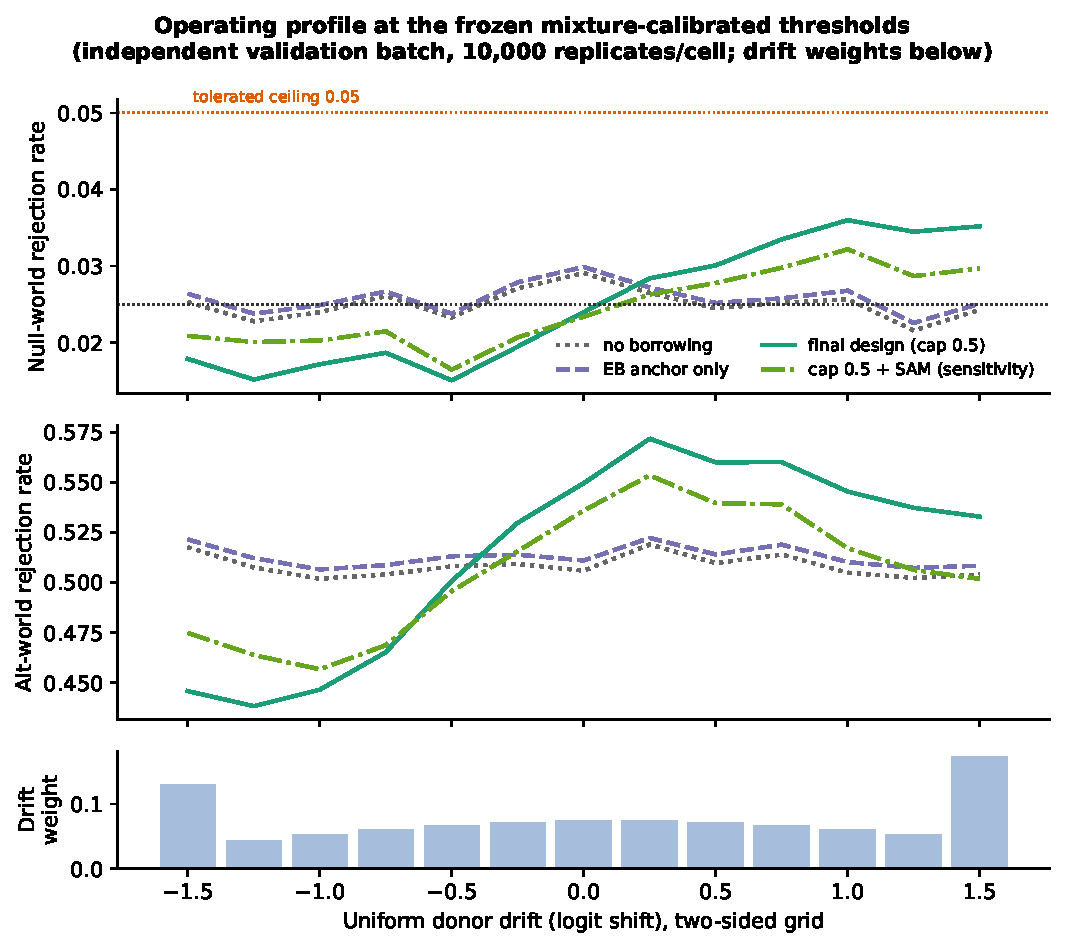
\includegraphics[width=0.9\textwidth]{F14_profiles}
  \caption{\textbf{Operating profile at the frozen mixture-calibrated
  thresholds} (independent validation batch, $10{,}000$ replicates per
  cell). Type I error (top) and power (middle) across the
  two-sided uniform drift grid for calibrated no borrowing, the EB anchor
  alone, the final design (cap $0.5$), and the SAM sensitivity variant; the
  empirical drift weights (bottom) show how the corpus distributes over the
  grid. The final design's power gain concentrates at small-to-moderate
  non-negative drift; its type~I error stays below the
  pre-specified $0.05$ ceiling everywhere.}
  \label{fig:profiles}
\end{figure}

\begin{table}[htbp]
\centering
\small
\caption{Design-based operating characteristics from the gold-standard
simulation ($2000$ replicates per cell). Single-arm design testing
$H_0\!:\theta \le 0.20$ at the one-sided $0.025$ level. Type I error is the
rejection rate in the null world ($\theta_0 = 0.20$); power is the rejection
rate in the alternative world ($\theta_0 = 0.35$). Columns are the
historical-versus-current logit shift. Monte Carlo standard errors are at most
$0.011$. UIP-JS uses the current trial's outcome and is not available at design
time. Alternative-world rejection at high conflict shifts is partly borrowed
bias rather than usable power (the same upward displacement that inflates the
null rejection rate), so the high-shift power of the standalone selective
prior ($0.836$ at shift $1.5$) should be read jointly with its null-world
column, not as a benefit.}
\label{tab:design-oc}
\begin{tabular}{lcccccccc}
\hline
 & \multicolumn{4}{c}{Type I error} & \multicolumn{4}{c}{Power} \\
Method & $0.0$ & $0.5$ & $1.0$ & $1.5$ & $0.0$ & $0.5$ & $1.0$ & $1.5$ \\
\hline
No borrowing                    & 0.037 & 0.029 & 0.034 & 0.028 & 0.536 & 0.544 & 0.561 & 0.546 \\
EB-only reference               & 0.030 & 0.022 & 0.032 & 0.022 & 0.497 & 0.514 & 0.526 & 0.511 \\
Rule mixture                    & 0.029 & 0.030 & 0.050 & 0.049 & 0.556 & 0.609 & 0.635 & 0.624 \\
Rule + SAM                      & 0.030 & 0.030 & 0.048 & 0.042 & 0.555 & 0.600 & 0.603 & 0.579 \\
Two-head + prospective          & 0.025 & 0.039 & 0.072 & 0.061 & 0.588 & 0.628 & 0.627 & 0.606 \\
Two-head + pro.\ + SAM          & 0.029 & 0.040 & 0.070 & 0.051 & 0.588 & 0.622 & 0.600 & 0.571 \\
Two-head + pro., fixed disc.    & 0.027 & 0.032 & 0.056 & 0.057 & 0.573 & 0.620 & 0.643 & 0.625 \\
Selective (prospective)         & 0.024 & 0.056 & 0.145 & 0.243 & 0.613 & 0.700 & 0.766 & 0.836 \\
Selective (no prospective)      & 0.026 & 0.046 & 0.110 & 0.185 & 0.599 & 0.685 & 0.752 & 0.821 \\
Selective, fixed discount       & 0.025 & 0.035 & 0.079 & 0.108 & 0.586 & 0.656 & 0.734 & 0.782 \\
Selective + SAM (anchored)      & 0.029 & 0.041 & 0.070 & 0.046 & 0.594 & 0.616 & 0.582 & 0.548 \\
Robust-MAP ($w=0.5$)            & 0.037 & 0.035 & 0.047 & 0.043 & 0.575 & 0.603 & 0.609 & 0.596 \\
UIP-JS (uses outcome)           & 0.050 & 0.048 & 0.069 & 0.081 & 0.625 & 0.670 & 0.721 & 0.737 \\
Power prior ($a_0=0.3$)         & 0.484 & 0.701 & 0.863 & 0.936 & 0.861 & 0.917 & 0.970 & 0.991 \\
Full pooling                    & 0.584 & 0.777 & 0.904 & 0.959 & 0.880 & 0.930 & 0.974 & 0.993 \\
\hline
\end{tabular}
\end{table}

\begin{figure}[htbp]
  \centering
  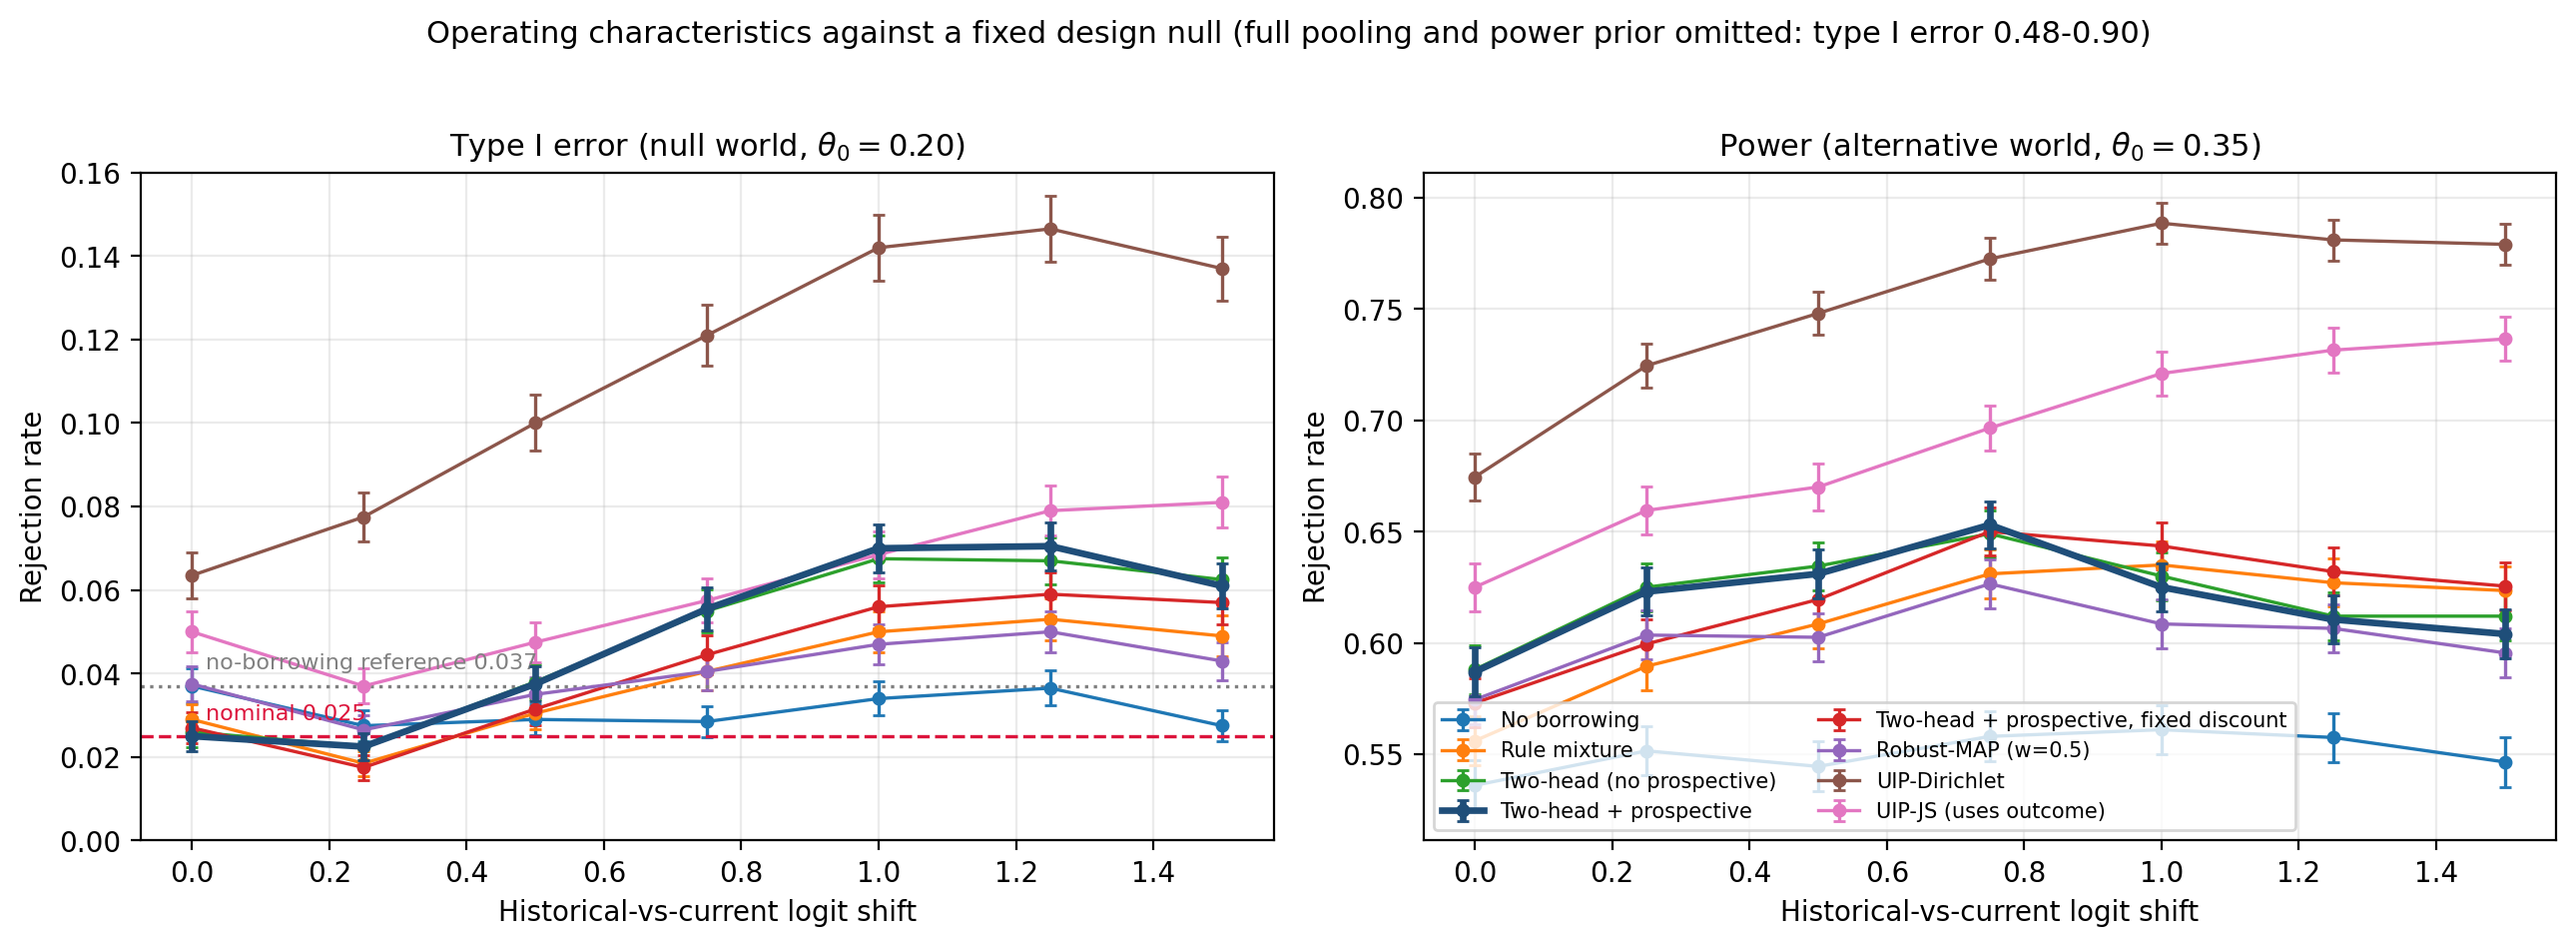
\includegraphics[width=\textwidth]{F8_design_oc}
  \caption{\textbf{Design-based operating characteristics.} Type I error (left,
  null world $\theta_0 = 0.20$) and power (right, alternative world
  $\theta_0 = 0.35$) against increasing prior-data conflict. The dashed red line
  is the nominal $0.025$; the dotted grey line is the no-borrowing rejection
  rate, which is the level actually achievable given binomial discreteness at
  these sample sizes. Full pooling and the power prior are omitted from the
  panel because their type I error ($0.48$ to $0.90$) is off scale.}
  \label{fig:design-oc}
\end{figure}

Scenario S1, in which almost all donors are exchangeable, was included
specifically to give the simple pooled competitors a favourable setting. The
learned prior still attained the lowest RMSE there ($0.0575$ versus $0.0726$
without borrowing and $0.0667$ for robust-MAP), while full pooling and the power
prior achieved worse RMSE ($0.1272$, $0.1132$) with coverage collapsing to
$0.271$ and $0.486$; their apparent efficiency comes at the cost of validity even
when their exchangeability assumption is close to satisfied.

\subsection{What the prospective conflict signal does and does not do}
\label{sec:prospective-results}

This analysis is reported in full, with its two figures, in
Supplement~S4; the findings, unchanged from the previous revision, are
summarised here because the repositioned paper relies on them. The
prospective set-level conflict signal does \emph{not} improve
borrowing-discrimination ROC-AUC (changes $-0.000$ to $+0.017$ across
scenarios, within Monte Carlo error) and cannot: it measures deviation
from the candidate-set consensus, so uniform whole-set displacement moves
the consensus with the conflict and is structurally invisible to it ---
under such conflict every design-time method's ROC-AUC falls below chance
($0.43$--$0.45$ in scenario S4; outcome-using UIP-JS reaches $0.813$). In
the fixed-budget architecture the signal is nevertheless what activates
the per-source discount head (borrowed size declining $31.3 \to 23.6$
with true distance, versus flat at $\approx 43.7$ without it); in the
selective architecture even that role disappears --- the discount
response is flat again, adaptivity migrates entirely to the set-level
total-borrowing head, and per-donor discrimination is no better than the
fixed-budget model's. This is the structural reason the final design
pairs the learned set-level decision with an explicit mixture-mass cap:
uniform displacement deceives the total-borrowing head, design-time
features cannot see it, and something outcome-free must attenuate the
consequences.

\subsection{External control arm}
\label{sec:ec-results}

Table~\ref{tab:ec} and Figure~\ref{fig:ec} report the hybrid-control scenario.
When external controls were substantially worse than the internal control
(logit drift $-1.2$) and there was no true treatment effect, using the internal
control alone gave a type I error of $0.013$ (MCSE $0.003$), reflecting the
conservatism of a small control arm under a flat prior. Full pooling reached
$0.210$ and the power prior $0.150$ --- a sixteen- and eleven-fold inflation
over the internal-only analysis --- with the hybrid
control rate biased downward by $-0.044$ and $-0.039$. The fixed-budget
two-head prior with
the prospective signal held type I error to $0.031$ while borrowing a nominal
$57$ patients; the fixed-discount ablation reached $0.025$ with a nominal $23$.

The selective prior behaved differently, and instructively: trained on an
external-control world in which half the candidate pool is drifted, it learned
to withhold borrowing almost entirely (nominal borrowed size $\approx 0$), and
its operating characteristics coincide with the EB-only reference at every
drift level (type I error $0.010$--$0.019$ across the grid, control bias
$-0.004$). Because the EC training draw has fairly homogeneous control rates,
the EB anchor itself is informative there ($\mathrm{Beta}(19.0, 78.7)$), and
that anchor --- not the external controls --- is what lifts power to $0.631$
versus $0.237$ for the flat-prior internal-only analysis in the
no-drift alternative world. Real control-rate heterogeneity is larger than
this training draw's, so we read the result as qualitative: given a
conflict-rich training distribution, the selective total-borrowing head is
capable of learning that external controls of this kind should mostly not be
borrowed, which is itself the design-relevant behaviour, while its candidate
\emph{ranking} remained the best among design-time methods (primary-label
ROC-AUC $0.642$).

\paragraph{Anchor misspecification: the EC safety is the anchor's, not the
method's.} Because a prior that borrows nothing inherits the operating
characteristics of its anchor, we stress-tested the anchor itself
(Table~\ref{tab:ec-anchor}): mean shifted by $\pm 0.4$ on the logit scale,
precision scaled $\times 4$ and $\times 1/4$, a flat $\mathrm{Beta}(1,1)$,
and new worlds in which the true control rate is heterogeneous across
replicates (SD $0.3$ on the logit scale). The selective prior's rows coincide
with EB-only's everywhere, which is the point: its favourable EC behaviour is
entirely the anchor's. A mis-centred anchor ($-0.4$ logit) inflates type I
error to $0.104$--$0.126$ at every drift --- an informative background prior
below the true control rate is exactly as dangerous as drifted external
controls, with none of the visibility; an over-precise anchor reaches
$0.033$ ($0.076$ under heterogeneity); and heterogeneity alone lifts even the
correctly centred anchor to $0.041$--$0.049$, confirming that the
homogeneous-control world flattered it. The only variant that is
simultaneously safe in every cell (type I $\le 0.029$ including
heterogeneity) and useful (power $0.433$ versus $0.237$ internal-only) is
the deliberately \emph{weakened} anchor (precision $\times 1/4$). The
constructive reading for hybrid-control designs is to down-weight the
marginal anchor rather than trust its fitted precision; the cautionary
reading is that ``the selective prior held type I error in the EC world''
is a statement about one well-specified anchor in one homogeneous world,
and we no longer present it as evidence of method-level safety. Two scopes
must not be conflated, and we are explicit about which this battery is: it
probes \emph{systematic misspecification} of the anchor, not the sampling
uncertainty of fitting it. The latter is quantified separately by a
nonparametric bootstrap of the anchor fit over the $500$-resample EC
training draw: the fitted anchor's logit mean varies within $\pm 0.06$
($95\%$ range) and its precision ratio within $0.70$--$1.24$ --- an order
of magnitude inside the battery's $\pm 0.4$ and $\times 4$ perturbations
--- and propagating that sampling uncertainty into the evaluation (one
bootstrap anchor drawn per replicate) leaves every operating
characteristic unchanged to Monte Carlo precision (null-cell type~I error
$0.011$--$0.019$ versus $0.010$--$0.019$ canonical; heterogeneity cells
$0.036$--$0.044$ versus $0.041$--$0.049$). Anchor-fit sampling
uncertainty is therefore not the risk; systematic mis-centring, over-fit
precision, and unmodelled control-rate heterogeneity are, and none of
them is a claim this battery ``accounts for'' in the propagation sense.

\begin{table}[htbp]
\centering
\small
\caption{External-control anchor-misspecification battery ($2{,}000$
replicates per cell). Type I error of the EB-only / selective prior (their
rows coincide: the selective prior borrows essentially nothing here) under
perturbed anchors, across the drift grid; ``het'' columns are new worlds
with the true control rate heterogeneous across replicates (SD $0.3$,
logit scale). Internal-only reference: $0.013$--$0.021$ across drifts
($0.015$--$0.019$ under heterogeneity). Power is in the no-drift
alternative world (heterogeneous-world power in parentheses).}
\label{tab:ec-anchor}
\begin{tabular}{lccccc}
\hline
Anchor variant & Worst T1 (drift grid) & T1 het $-0.8$ & T1 het $0.0$ & Power & \\
\hline
Canonical $\mathrm{Beta}(19.0,78.7)$ & 0.019 & 0.049 & 0.041 & 0.631 & (0.617) \\
Mean $+0.4$ logit                    & 0.001 & 0.005 & 0.009 & 0.229 & (0.284) \\
Mean $-0.4$ logit                    & 0.126 & 0.166 & 0.150 & 0.878 & (0.862) \\
Precision $\times 4$                 & 0.033 & 0.076 & 0.072 & 0.730 & (0.704) \\
Precision $\times 1/4$               & 0.021 & 0.029 & 0.022 & 0.433 & (0.459) \\
Flat $\mathrm{Beta}(1,1)$            & 0.021 & 0.019 & 0.015 & 0.237 & (0.241) \\
\hline
\end{tabular}
\end{table}

Robust-MAP achieved a low type I error among borrowing methods ($0.015$),
but its false-positive rate for borrowing non-comparable external controls was
$1.000$: it does not discriminate at all, and its safety comes entirely from
borrowing very little (nominal borrowed sample size $7.7$). The fixed-budget
two-head prior had a
false-positive rate of $0.58$ while borrowing seven times as much information.
UIP-JS achieved the best discrimination ($0.20$) but, again, only by using the
current outcome.

\begin{table}[htbp]
\centering
\small
\caption{External control arm, null world (no true treatment effect), external
controls displaced downward by a logit drift of $-1.2$; $2000$ replicates.
Type I error is the rate of declaring superiority. FPR is the proportion of
non-comparable external controls that were nonetheless borrowed
(primary parameter-level labels; shown as --- for the selective prior, which
places essentially zero mass on candidates here, so the borrowed/not
binarisation is vacuous). Control bias is
the posterior mean of the hybrid control rate minus its true value; a negative
value means the borrowed controls dragged the control estimate down, which is
what inflates the apparent treatment effect.}
\label{tab:ec}
\begin{tabular}{lccccc}
\hline
Method & Type I error & (MCSE) & Control bias & Nominal borrowed size & FPR \\
\hline
Internal control only            & 0.013 & (0.003) & $+0.028$ & 0.0   & 0.00 \\
EB-only reference                & 0.018 & (0.003) & $-0.004$ & 0.0   & 0.00 \\
Rule mixture                     & 0.021 & (0.003) & $+0.003$ & 18.9  & 0.61 \\
Two-head + prospective           & 0.031 & (0.004) & $-0.007$ & 56.7  & 0.58 \\
Two-head + prospective + SAM     & 0.031 & (0.004) & $-0.004$ & 53.8  & 0.58 \\
Two-head + pro., fixed discount  & 0.025 & (0.004) & $-0.002$ & 22.6  & 0.53 \\
Selective (prospective)          & 0.018 & (0.003) & $-0.004$ & 0.0   & --- \\
Selective + SAM (anchored)       & 0.018 & (0.003) & $-0.004$ & 0.0   & --- \\
Robust-MAP ($w=0.5$)             & 0.015 & (0.003) & $+0.010$ & 7.7   & 1.00 \\
UIP-JS (uses outcome)            & 0.066 & (0.006) & $+0.000$ & 9.4   & 0.20 \\
Power prior ($a_0=0.3$)          & 0.150 & (0.008) & $-0.039$ & 228.1 & 1.00 \\
Full pooling                     & 0.210 & (0.009) & $-0.044$ & 760.5 & 1.00 \\
\hline
\end{tabular}
\end{table}

\begin{figure}[htbp]
  \centering
  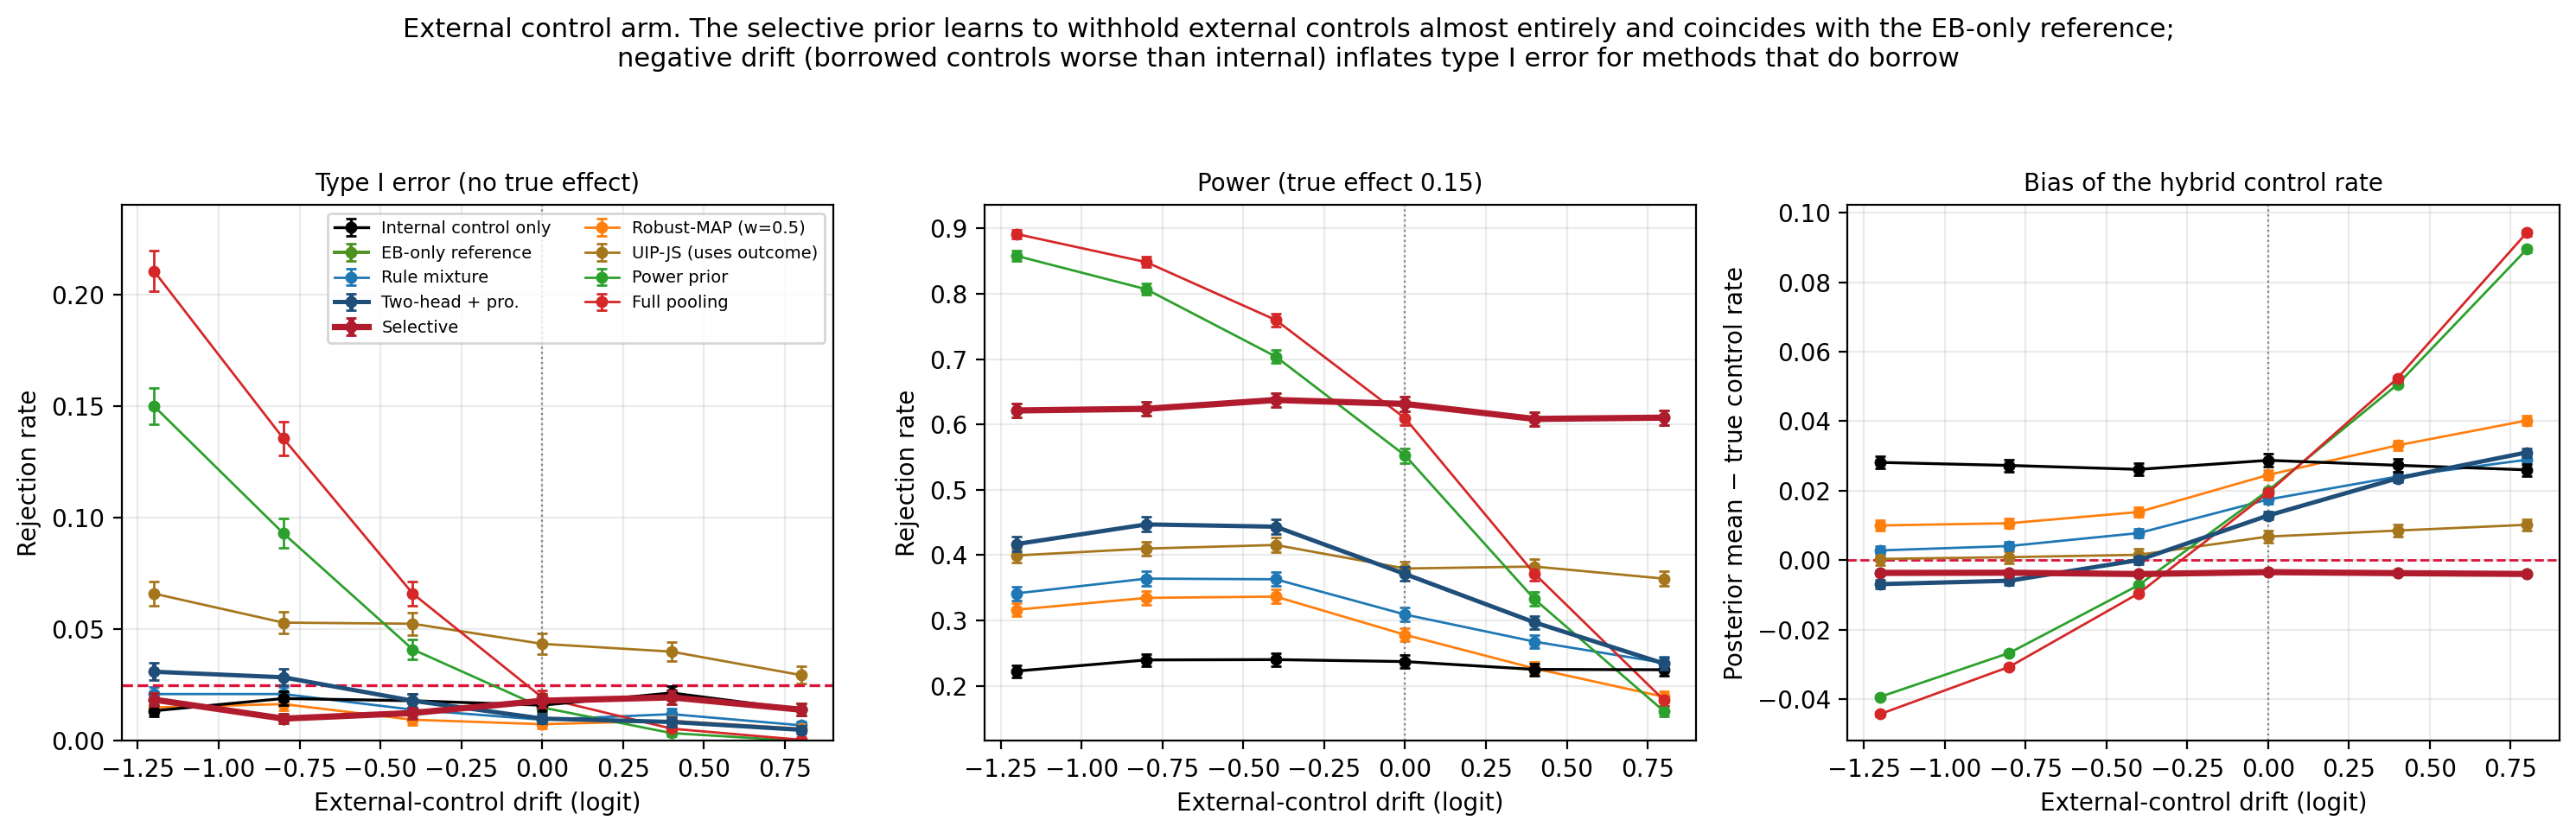
\includegraphics[width=\textwidth]{F11_external_control}
  \caption{\textbf{External control arm operating characteristics.} Type I
  error (left), power (centre) and bias of the hybrid control rate (right) as
  the external controls drift away from the internal control. Negative drift
  means the borrowed controls are worse than the internal control, which biases
  the treatment effect upward. The dashed red line in the left panel is the
  nominal $0.025$.}
  \label{fig:ec}
\end{figure}

The practical reading is that in the external-control setting the quantity that
governs type I error inflation is how much is borrowed at least as much as how
well donors are selected. Under the worst simulated drift ($-1.2$), every
method that actually borrowed exceeded the internal-only rejection rate
(pointwise, some cells elsewhere on the grid sit below $0.025$); methods that
borrowed essentially nothing (EB-only, the selective prior) matched the
reference --- safety by abstention, not by successful selection, and, as the
anchor-misspecification battery below shows, safety that is only as good as
the anchor. This is consistent with regulatory caution about external
controls [8] and with the causal framing of recent reviews [18].

We had also planned a worked external-control case study on real registry data,
mirroring the two ORR case studies. It is not reported here. Constructing it
requires arm-level control outcomes, and auditing the corpus for that purpose
uncovered the endpoint-unit defect described in
Section~\ref{sec:limitations-data}, which affects a subset of arm-level rate
extractions. We judged it wrong to build a new worked example on an extraction
path we had just found to be unreliable, and have deferred it until the
corrected extraction has been re-run end to end.

% ---------------------------------------------------------------------

% ---------------------------------------------------------------------
\section{Case studies}
\label{sec:casestudies}
To make the pipeline concrete we walk through two leakage-controlled
pseudo-queries end to end --- recomputed, like every real-data number in this
paper, on the unit-corrected data with the final models. They were chosen
before the selective architecture existed, and they turned out to illustrate
the two sides of the selectivity story: one query where compatible historical
evidence sharpens the prediction, and one where the marginal reference is the
better bet and the selective model correctly withholds most of its borrowing.

\paragraph{Case 1 (borrowing helps; development-set illustration).}
NCT02551432, a completed single-arm Phase~2
trial of pembrolizumab plus paclitaxel in relapsed/refractory small-cell lung
cancer, had its objective response held out and hidden from retrieval,
reranking, and feature construction (true outcome 6 of 26, observed ORR
$0.231$; this query fell in the training split, so learned rows here are a
development-set illustration). Stage~1--2 admitted six endpoint-compatible
historical arms with usable result tables. As Table~\ref{tab:case}
shows, the flat prior predicts poorly (NLL $3.296$) and the EB reference
improves on it ($3.010$); borrowing helps further --- the rule prior reaches
$2.890$, the selective prior $2.844$ (borrowing $0.46$ of its mass), and the
fixed-budget model, which happens to be right to borrow heavily here, $2.780$.
This is a single retrospective
illustration, not a clinical endorsement: the donors were selected for endpoint
compatibility and result usability rather than adjudicated exchangeability, and
one favorable case does not establish borrowability.

\begin{table}[htbp]
\centering
\caption{Worked case study (NCT02551432, held-out ORR $6/26 = 0.231$;
development-set illustration). Predicted
response rate and held-out beta-binomial NLL for each design-time prior on
this single query. Compatible historical arms sharpen the prediction beyond
the EB reference.}
\label{tab:case}
\begin{tabular}{lrrc}
\toprule
Prior & Predicted ORR & Held-out NLL & 95\% interval covers truth \\
\midrule
Weak-only $\mathrm{Beta}(1,1)$ & 0.500 & 3.296 & yes \\
EB reference (no borrowing) & 0.284 & 3.010 & yes \\
Rule prior & 0.377 & 2.890 & yes \\
Selective (borrowed mass $0.46$) & 0.267 & 2.844 & yes \\
Two-head, fixed budget ($0.80$) & 0.285 & \textbf{2.780} & yes \\
\textit{Observed (held out)} & \textit{0.231} & --- & --- \\
\bottomrule
\end{tabular}
\end{table}

A second worked example --- NCT03046953, a held-out test-split query where
borrowing is \emph{not} clearly warranted --- shows the complementary
behaviour and is reported in full in Supplement~S3: the fixed-budget model,
forced to place $0.80$ of its mass on the candidates, does worse than the
EB reference ($3.182$ vs $3.026$), while the selective model borrows only
$0.40$ and lands within $0.021$ of the reference --- the triage behaviour
of Section~\ref{sec:triage-results} at the level of a single query. Read
together, the two case studies show both halves of the intended
behaviour: borrowing taken up where compatible evidence sharpens the
held-out prediction (Case~1), and largely withheld where the marginal
reference is the better bet, limiting the damage that a forced borrowing
budget would otherwise cause (Supplement~S3). Outcome-adaptive SAM rows
are omitted
here under the partition rule of Section~\ref{sec:eval}; the aggregate
counterpart of this per-query behaviour --- borrowing helping under
exchangeability and doing harm under conflict --- is what the gold-standard
simulation operating characteristics (Section~\ref{sec:goldsim-results}) and the
external-control analysis (Section~\ref{sec:ec-results}) quantify in aggregate.

\section{Discussion}

This study presents an explainable methodology prototype for moving from
oncology trial similarity to Bayesian historical borrowability. The central
contribution is not a new text-retrieval model alone, but a pipeline that
links retrieval, candidate-level borrowability features, endpoint observation
extraction, beta-binomial mixture components, retrospective calibration,
prior-data conflict adaptation, and simulation operating-characteristics
evaluation. This addresses a common gap in historical-borrowing workflows:
retrieved historical trials are often treated as similar before the
statistical consequences of borrowing are assessed.

The results support several bounded observations, and the most important is
also the most cautionary. First, \emph{marginal empirical-Bayes references are
hard to beat}: judged against a two-parameter intercept-only EB prior rather
than a flat $\mathrm{Beta}(1,1)$, every fixed-budget borrowing construction we
evaluated --- rule-weighted, power-prior-, MAP- and commensurate-style, tuned
robust-MAP, and our own earlier fixed-budget learned model --- delivered
\emph{no} average real-data benefit, and most were significantly worse. Much
of the apparent benefit of borrowing in flat-referenced comparisons, our own
earlier drafts included, is marginal-distribution information in disguise.
Second, \emph{selectivity plus an explicit cap is what earns back the
difference, and the observed value is harm attenuation}: making
the total borrowing learnable per query, anchored at the EB fit, produced a
significant paired improvement over the fixed-budget architecture in and out
of time (robust to donor-block resampling), the only design-time prior at or
below the EB reference, and calibration
approaching the EB reference at lower NLL; capping that learned total at
$0.5$ then \emph{improved} the out-of-time results further (the capped
forward and title-screened deltas are the tiers' only significant
selective-versus-EB intervals) while converting the primary analysis from
harmful to neutral --- gaining where
the premise holds and attenuating (not eliminating: pointwise error
inflation up to and, under anchor-precision stress, beyond the tolerated
ceiling remains) losses where it fails; all capped real-data numbers are
post hoc redesign evaluations in the sense of
Section~\ref{sec:forward-results}. The learned
mass ranks
the realized benefit of borrowing on unseen data (rank correlation $+0.16$,
stable across windows), and where it is low the forced-borrowing damage of
the predecessor ($+0.148$ against EB) is eliminated to neutrality
($+0.003$); superiority where information is rich remains directional rather
than demonstrated. Third, \emph{what could be borrowed and what had been
posted are different populations}: under the registry-availability proxy at
each query's design date, most historical results were not yet
posted, predictive gains are undemonstrated (and the
availability-consistently trained model is harmful where it borrows), and
the framework's
addressable population is best understood as growing with registry maturity
--- $31\%$ of latest-window queries already have an available gated donor ---
rather than as the whole retrospective corpus. Fourth, the known-truth
simulation now cuts both ways for the revised architecture: under
exchangeability the selective prior attains the highest observed power
among methods whose \emph{estimated} type I error was $\le 0.025$ in that
cell (a Monte Carlo statement at $2{,}000$ replicates, not proof of
control), but its learnable total borrowing
removes the fixed budget's accidental cap, its standalone type I error
escapes under uniform whole-set conflict ($0.243$ at the strongest shift),
and its per-source discount response is flat; no companion restores strict
control --- the anchored SAM adapter only mitigates the inflation (worst
case $0.070$), and the explicit mixture-mass cap of the final design
attenuates it ($0.044$ at standard settings, but $0.0595$ under
anchor-precision stress; the drift-averaged behaviour is characterised
only in the exploratory decision analysis) --- while in the
external-control world, trained on a conflict-rich draw, the same head
learns to withhold external controls almost entirely, with operating
characteristics that the anchor stress-test battery shows belong to the
anchor. These
simulation analyses do not
establish clinical exchangeability or expert borrowability.

A fifth observation states the evidence boundary of the complete proposal
explicitly. In the previous revision the proposal's two components were
validated in systems that did not compose: the design-time prior had
real-data predictive evidence but no standalone frequentist safety (its
uncalibrated conflict inflation reaches $0.243$ and no threshold in the
searched range rescues it --- extending the search toward $1$ only reaches
control at thresholds where power has collapsed below the no-borrowing
reference, so the rescue is degenerate, not absent by artefact), while the
SAM companion had simulation evidence but could not be scored on real data.
The final design resolves that composition problem \emph{structurally}: the
mixture-mass cap is a deterministic design-time projection, so the capped
selective prior is one and the same object in both evidence systems --- on
real data it is predictively neutral in the primary analysis and
significantly better
than the EB reference on the title-screened upper-bound tiers (post hoc
redesign evaluations throughout), and in
known-truth simulation its worst-case behaviour is measured against a
declared tolerance and its drift-averaged behaviour is characterised in an
exploratory decision analysis. What
remains outside any single evidence stream is expert-level donor
discrimination (not demonstrated anywhere) and strict worst-case safety
with power benefit (unavailable to any borrowing method in one-parameter
settings of this kind [28]). A sixth
observation grades the effectiveness claim by frame, and we commit to this
grading wherever the method is described: \emph{cell by cell}, the
ROC-efficiency diagnostic --- which conditions on the unknown true drift
and is therefore not an implementable power benefit --- locates a real
local advantage at small drift of either sign ($\approx +0.07$ near zero,
fading through $|{\rm drift}| \approx 0.75$, reversing beyond
$|{\rm drift}| \approx 1$); \emph{averaged over the drift actually
observed in this corpus, size-adjusted}, all single-analysis point
estimates were positive but the sign is not established once
threshold-estimation uncertainty is considered (repeated cross-fit:
$-0.0007$, $95\%$ split interval $[-0.0014,+0.0039]$), with only the
dispersion dependence robust; \emph{under adversarial
drift} no design-time method retains a benefit, ours included, and the cap
attenuates --- it does not provably bound --- the cost
of being wrong.

These findings locate the contribution against each of the three families
surveyed in the Introduction. Relative to the statistical borrowing literature
--- power priors, commensurate priors, MAP and robust-MAP constructions, and
SAM [3,~4,~5,~6,~11] --- we do not take the historical set as given: the
pipeline selects candidates and then weights them, separates the
allocation decision (the mixture weight $\lambda_i$) from the information-size
decision (the discount $a_i$), and learns whether to borrow at all, three
quantities those methods typically collapse into one or two. The empirical
form the argument takes here is deliberately strict: a tuned robust-MAP prior
beat flat-anchored borrowing but not the plain EB reference, whereas the
selective model did --- so the case for candidate-level machinery now rests on
selectivity, not on borrowing as such; the closest precedent for per-source
adaptive weights is the unit
information prior of Jin and Yin [19], which we implement and evaluate directly
rather than describe. Relative to machine-learning trial-outcome prediction, the
reranker and the conservative clinical gate are inspectable feature by feature
and the output is a calibrated prior distribution rather than a predicted
label, so the borrowing decision can be audited at the level at which it is
made. Relative to text-similarity retrieval [12,~13,~14], the pipeline adds the
borrowability layer that similarity alone cannot supply, and --- the point on
which we would rest the case --- submits that layer to predictive calibration
rather than assuming it is correct.

The simulation study complements retrospective calibration by examining
operating characteristics under controlled exchangeability and conflict
scenarios. Optimistic historical conflict increased apparent power but also
increased bias and reduced coverage; the SAM-style adapter showed higher
trigger rates under stronger conflict, supporting its role as a transparent
sensitivity mechanism. These findings are consistent with the broader
principle that historical borrowing should be evaluated not only for
predictive fit but also for conflict behavior and decision operating
characteristics [5,~10,~11].

\subsection{A defect in endpoint-unit handling: discovery, scope, and correction}
\label{sec:limitations-data}

While auditing the corpus in preparation for the external-control case study we
found a defect in how arm-level outcome rows were converted into rates. The
extraction divided the reported value by the arm denominator unconditionally.
That is correct when ClinicalTrials.gov reports an outcome as a participant
count, but not when it reports the same outcome as a percentage or a proportion,
which it frequently does for objective response rate. A row reading $26.0$ with
denominator $31$ under the unit ``Percentage of Participants'' denotes an ORR of
$0.26$, whereas the defective extraction produced $0.839$.

We report the scope precisely. Of $3319$ arm-level ORR rows in the corpus,
$2040$ are reported in percentage units and $846$ in participant counts; $804$
rows ($24.2\%$) were assigned a rate above $1$, which is self-evidently
impossible, while the remainder of the affected rows produced values inside
$(0,1)$ that look plausible and are correspondingly more dangerous. Within the
pre-correction borrowing dataset, $9$ of $93$ locatable query outcomes changed
under corrected handling, $8$ of them by more than $0.10$ in absolute rate, the
largest by $0.579$. The
held-out query outcome is the reference against which predictive NLL,
calibration and coverage are computed, and historical component observations
$(y_i, n_i)$ enter every prior directly, so the pre-correction real-data
aggregates were contaminated on both sides: pre-correction training examples
contained fractional ``responder counts'' (percentage values passed through
unconverted, such as $52.3$ of $65$), proportion-reported query outcomes
truncated to zero by integer casting, and percentage rows silently dropped
whenever the reported value exceeded the denominator.

The conversion was corrected at all four call sites to dispatch on the
reported unit of measure, reconstructing responder counts for
percentage-reported rows as $\mathrm{round}(\text{rate} \times n)$ (an error of
at most half a participant, flagged in the data) and refusing to convert rows
whose unit is missing or unrecognised ($29$ rows) rather than guessing. Because
the stored corpus retains the reported unit for every arm-level row, and
because the unit conversion enters neither Stage~1 retrieval nor Stage~2
reranking scores, the full downstream evaluation was regenerated from the
stored pipeline results without re-running retrieval: the same $1{,}470$
leakage-controlled pseudo-queries now yield $1{,}407$ usable examples
(previously $1{,}414$; some queries lost their only convertible row under
strict unit handling while previously dropped percentage rows re-entered). All
real-data numbers reported in this manuscript --- the head-to-head, robust-MAP,
calibration, and forward-validation analyses --- come from the corrected
re-run, executed with the same seeds and pinned environment.

The correction moved NLL levels down for every method (the held-out reference
outcomes are cleaner) while preserving method orderings within the
then-current comparisons, and forward-validation improvements at the time
remained stable with paired bootstrap confidence intervals excluding zero. The
correction also motivated the sharper evaluation reported in this version:
cleaner targets made it possible to fit a meaningful empirical-Bayes
reference, against which the limits of fixed-budget borrowing --- and the case
for the selective architecture --- became visible. Three
things were never affected. The held-out outcomes of the two worked case
studies (Section~\ref{sec:casestudies}) are reported in participant units
($6/26$ and $5/32$) and were never corrupted; their prior computations, like
every real-data analysis, were regenerated on the corrected data with the
final models. The gold-standard simulation and
the external-control simulation do not touch this extraction path at all. And
the direction of the defect was not systematically favourable to our method: it
perturbed the held-out truth for a minority of queries in both directions. The
audit table identifying every affected query, the pre-correction artifacts, and
the corrected regeneration scripts are released with the code so the effect of
the correction is itself reproducible.

We record this in the main text rather than a supplement because a defect that
silently produces plausible-looking numbers is precisely the kind that a reader
cannot detect from reported results alone.

\paragraph{Manual registry audit.} A manual audit of $80$ extracted
observations --- $60$ donor observations from the forward windows and $20$
query outcomes, stratified to oversample percentage-derived rows ($42$) and
the ten most-shared donors (a census of that stratum), each checked against
the live registry on six
items --- completes the extraction-quality picture, and its two halves point
in opposite directions. The audit was performed by a single author-auditor
against the current registry records, without independent duplicate
extraction or adjudication; we therefore describe it as a single-rater
author audit rather than an expert panel, and report design-weighted
corpus-level estimates (stratum sampling fractions applied; finite-population
correction for the census stratum) alongside the raw sample rates.
\emph{Numeric} integrity is high: raw sample rates --- arm identification
$98.8\%$, numerator $97.5\%$, denominator $97.5\%$, analysis population
$97.5\%$; all four simultaneously, $93.8\%$ ($95\%$ CI $86.2$--$97.3\%$)
--- and design-weighted corpus-level estimates of the same joint numeric
integrity: $93.5\%$ (CI $87.1$--$100\%$) for donor observations and
$100\%$ (all $20$ audited) for query outcomes. The
percentage-reconstruction path introduced by the unit correction was
specifically vindicated where the borrowing gains concentrate: in the
percentage-derived stratum, denominator and analysis-population agreement
were $42/42$ and the numerator $41/42$ (one integer-rounding ambiguity). The
audit found two numeric errors. One is a genuine two-stage parse failure on a
proportion-scale row: a registry cell posted as ``.1 (0.6\%)'' was stored
upstream as a count of $1.0$, which the proportion-unit reconstruction then
read as $100\%$ of $18$ --- one candidate observation in one query; a
value-consistency guard now flags this pattern, and identified two further
unverifiable $100\%$-proportion rows. The other is registry-version drift on
the single most-shared donor: our snapshot stores $4/12$, internally
consistent with its then-posted ``4 (33.3\%)'', while the current registry
reports the same four responders over $13$ --- an instance of the
as-of-snapshot limitation of Section~6.2 rather than a parser error, but one
touching $307$ examples. Correcting both errors and dropping the flagged
rows changes the headline comparisons by less than $0.001$ NLL (test
$\Delta$ vs EB $-0.0295 \to -0.0298$; forward $-0.0266 \to -0.0273$): the
conclusions are insensitive to every numeric error the audit found.

The dominant discordance is \emph{semantic}, not numeric. Agreement that the
extracted endpoint is strictly an objective response rate (CR+PR or a
disease-appropriate equivalent) was $77.5\%$ in the sample ($62/80$; CI
$67.2$--$85.3\%$); design-weighted, $75.9\%$ (CI $64.6$--$87.1\%$) of donor
observations and $70.4\%$ (CI $52.7$--$88.1\%$) of query outcomes ---
internally consistent with the canonicaliser's corpus-level rate of
$73.1\%$ (Section~\ref{sec:eval}), though the two are not independent
corroboration: the canonicaliser's rules were informed by this same
audit. Agreement was
lower for count-reported rows ($60.7\%$) than percentage-reported ones
($83.3\%$): complete-response-only rates, clinical-benefit and pathological
response rates, composite remission and molecular-response endpoints, and in
one query a non-tumour ``complete response'' (absence of emesis after
chemotherapy) were admitted as ORR. The corpus endpoint is therefore better
described as a \emph{primary binary response-type endpoint} with roughly
three-quarters strict-ORR purity. Queries and donors carry the same heterogeneity,
so the predictive evaluation remains internally consistent, but
cross-family borrowing (a complete-response-only donor informing an ORR
query) contributes systematic distance that the endpoint gate only partly
captures; endpoint-definition canonicalisation --- parsing measure
descriptions rather than titles --- is the highest-priority data-quality
improvement this audit identifies. The completed audit table is released
with the code.

\paragraph{Out-of-sample endpoint audit.} Because the canonicaliser's rules
were iterated against the $80$-row audit above, a second, frozen-rule audit
was performed on $60$ fresh records (trials untouched by the first audit;
stratified by role $\times$ frozen prediction; predictions withheld from
the auditor; same single rater, judging against the registry's full
outcome descriptions). Two records were adjudicated indeterminate and set
aside. On the remaining $58$: accuracy $82.8\%$ (exact $95\%$ CI
$70.6$--$91.4$; corpus-weighted $81.9\%$), sensitivity $85.7\%$,
specificity $80.0\%$ --- confirming that the $98.6\%$ resubstitution figure
was optimistic, and quantifying by how much. The error anatomy is
informative on both sides. The six false positives are ``response
rate''-titled endpoints that are not tumour objective response ---
prostate-specific-antigen-based response (twice, one a PSA-or-radiographic
composite), bone-scan response, an
abscopal-lesion response, and two ``participants with a response'' titles
concealing haematologic CR-variant composites; the four false negatives
are conservatively excluded titles (``clinical response'', a vague
``assessment of tumour response'', a criteria-spelling variant) whose
registry definitions turn out to be genuine CR+PR objective response. The
positive predictive value, $80.0\%$ (CI $61.4$--$92.3$), is the measured
purity of the title-screened subset: enriched over the unscreened corpus's
roughly three-quarters, with the systematically biased families (pCR,
PFS-defined, disease-control, molecular) removed wholesale, but not pure.
The rules were not retuned on these errors; both audit tables and the
scoring script are released with the code.

\subsection{Limitations}
First, no expert borrowability labels were available; the evaluation cannot
establish that any individual retrieved historical trial is clinically
appropriate for borrowing. The reranking scores, compatibility gates,
borrowed-size discounts, and mixture weights are heuristic and unvalidated;
retrospective predictive calibration is not clinical validation, and expert
clinical and statistical review together with external validation are
prerequisites for any decision-informing use. Results should be interpreted as
retrospective predictive-calibration, simulation operating-characteristics,
and internal-validation evidence rather than expert adjudication or regulatory
qualification. Second, and more fundamentally, the design-time layer is not
sufficient on its own. Per-donor features computed before the current outcome is
seen describe design similarity only, and are in principle unable to identify a
prior--data conflict that displaces the entire retrieved set uniformly: the
consensus of the remaining donors moves with the displacement, so no donor
appears deviant. This is not a shortcoming of the particular signal we
constructed but a property of any criterion built, as ours is, from these
design features and within-set donor consensus --- an unmeasured uniform
displacement of the whole set is unidentifiable to it in principle --- and it
is visible in
the results: under such conflict (scenario~S4) the borrowing-discrimination
ROC-AUC of every design-time method we evaluated fell below chance
($0.43$--$0.45$ under the primary parameter-level labels), while UIP-JS,
which computes its weights against the current data, attained $0.813$
(Section~\ref{sec:prospective-results}). For the selective architecture this
is not an abstract caveat but a quantified failure mode: precisely because
its total borrowing is learnable, uniform conflict that design-time features
cannot see inflates its standalone type I error to $0.243$ at the strongest
shift we simulated --- four times the fixed-budget predecessor's --- and its
per-source discount response is flat, so nothing at the donor level
compensates. We therefore do not claim that
prospective selection can stand alone: the mixture-mass cap of the final
design is the component that attenuates this failure mode (worst case
$0.044$
against $0.243$ uncapped at standard settings, $0.0595$ under
anchor-precision stress --- attenuation, not a demonstrated bound), the
outcome-dependent SAM layer is a simulation-evaluated sensitivity analysis
for the uncapped prior that mitigates but does not eliminate the inflation,
and unrestricted worst-case calibration erases the net power benefit of any
borrowing method [28] --- the design's power case lives in the
empirical-mixture frame, whose own limitation is stated below
(Table~\ref{tab:calibrated}). Third, the availability-controlled primary
analysis of
Section~\ref{sec:primary-results} bounds what the forward validation can
claim: under the registry-availability proxy applied at each query's design
date, most
of the pooled advantage over the EB reference is not realisable, because the
donor results had not yet been posted, and the availability-consistently
trained model is harmful where it borrows. The proxy itself has two known
defects, both of which make it an approximation rather than a replay. It is
a trial-level date: it cannot certify that the specific endpoint row existed
in its current form at that date, and the stored registry records are
current versions rather than as-of-cutoff snapshots, so endpoint text edited
after completion can differ from what a contemporaneous user saw --- the
audit's most-shared donor ($4/12$ in our snapshot, $4/13$ today, touching
$307$ examples) is the concrete demonstration that snapshot reconstruction,
which remains future work, is needed for a true historical replay. And it
ignores the literature channel (results are often published before registry
posting); we have not implemented or validated a literature-retrieval
pipeline, so we treat this strictly as an unimplemented extension and do not
use it to discount the null primary result. Fourth, marginal
references set a high bar that should temper enthusiasm for borrowing
machinery in general: a disease-stratified EB prior matched the selective
model on the pooled forward windows (while being unstable across settings),
the \emph{uncapped} selective-versus-EB aggregate intervals include zero
under every resampling scheme we tried (query-level and donor-block
bootstrap alike; the capped final design's forward and title-screened
upper-bound intervals are the ones that exclude zero),
the information-subgroup threshold, though fixed before the final window was
examined, derives from exploratory analysis, and the aggregate advantage
concentrates in percentage-derived, recent, larger trials
(Section~\ref{sec:forward-results}); multi-seed stability and the
pre-registered seed-ensemble result are reported in
Section~\ref{sec:forward-results}. A related limitation attaches to the
empirical-mixture calibration itself: its mixing measure is estimated from
the same corpus the method is evaluated on (among gated, title-screened
donor--query pairs, with a method-of-moments deconvolution that leans on an
approximate normal law), so the mixture guarantee is relative to
\emph{this} corpus's drift profile, not a universal one; the worst-case
ceiling and the per-shift profile are reported precisely so a reader can
re-weight by their own prior over drift. Fifth, automated extraction from ClinicalTrials.gov introduces errors
that are now measured at two levels. The automated audit quantifies gross
invalidity (about 44\% of raw arm-level rows are not valid binary
observations; an admission rule passing a synthetic round-trip check removes
them), and the stratified single-rater author audit of Section~\ref{sec:limitations-data}
bounds the residual: numeric extraction in the admitted subset is
$93.8\%$ clean on all four numeric items jointly, the two errors found move
the headline comparisons by under $0.001$ NLL, but only $77.5\%$ of admitted
``ORR'' rows are strictly objective response rates --- endpoint-family
heterogeneity, not numeric corruption, is the main residual data-quality
limitation. The title-screened subset is the implemented mitigation, with
its own limitations stated in Section~\ref{sec:eval} (single-rater,
title-level, resubstitution-validated with a frozen-rule out-of-sample
check); description-level canonicalisation with independent dual-rater
adjudication remains the identified full fix.
Sixth, the framework and its evidence are limited to binary endpoints;
applying the full retrieval and two-head pipeline to progression-free survival
at fixed time points and other endpoints remains to be demonstrated. Seventh, the SECRET-style
backend is a deterministic section-based minimum viable product, and
Trial2Vec-style retrieval remains optional. Finally, simulation scenarios
simplify oncology-trial complexity and should be viewed as stress tests rather
than substitutes for protocol-specific operating-characteristics studies.

\subsection{Regulatory and practical implications}
Historical borrowing for decision-informing trials requires pre-specification
of evidence selection, prior construction, conflict assessment, and
operating-characteristics evaluation. These expectations are made explicit in
the FDA draft guidance on Bayesian methodology in drug and biologic trials
[16,~17], which calls for pre-specified success criteria and decision
thresholds, justified priors with quantified influence (for example, effective
sample size), simulation-based operating characteristics including type~I error,
prior sensitivity and prior-data-conflict analyses, and reproducible
computation; the ICH~E9(R1) estimand framework [9] and the external-controls
guidance [8], together with causal-inference framings of external borrowing
[18], impose related requirements. The present framework instantiates several
of these elements retrospectively: transparent, auditable candidate features; an
explicit separation of the mixture weight $\lambda_i$ from the
borrowed-size discount $a_i$, with the weighted nominal borrowed sample size
reported as bookkeeping (not a Morita-style prior ESS); simulation operating
characteristics with Monte Carlo standard errors and a prior-data-conflict
sweep; a prior-sensitivity and weight-tuning analysis; an explicit
mixture-mass cap with a calibrated threshold; and a pinned, reproducible
evidence package. We emphasize that this is
a retrospective methodological \emph{alignment with}, not a demonstration of
\emph{compliance under}, that guidance. Any use in a real trial would require
disease-specific expert review, endpoint-specific validation, protocol-level
pre-specification, and formal operating-characteristics evaluation tailored to
the intended decision. The repository should be used as a reproducible
methodology prototype and calibration evidence package, not a clinical borrowing
recommendation system.

% ---------------------------------------------------------------------
\section{Conclusion}
We developed a reproducible methodology prototype that separates three
questions usually merged in historical borrowing: whether a past trial
\emph{can be found} (retrievability), whether it \emph{should be borrowed
from} (borrowability), and \emph{how much to borrow at all}. The core
contribution is a selective two-head DeepSets model that, for each retrieved
candidate, learns a mixture weight and a separate information discount, and,
through a set-level head anchored at an empirical-Bayes prior, a per-query
total borrowing fraction --- an architecture that \emph{permits} ``which
donor,'' ``how much information,''
and ``whether to borrow'' to be decided separately. The evidence supports
less than the architecture permits: in the final selective model the
learned per-source discount response was empirically flat, and the
observed gain is attributable primarily to the EB anchor and the
set-level total-borrowing head.

Because expert borrowability labels do not exist at scale, we evaluated the
pipeline without them, against an intercept-only empirical-Bayes reference and
under a strict partition between design-time and outcome-adaptive priors:
held-out-split and disjoint-window forward NLL, calibration diagnostics,
robust-MAP and classical baselines, and gold-standard and external-control
simulations with known truth, alongside automated and single-rater extraction
audits. The
empirical accounting is deliberately unsparing, and the supportable
conclusion is precise, stated in the order of its evidential weight. The
primary real-data analysis --- registry-availability proxy on the
audit-informed, title-screened binary-response subset --- demonstrates \emph{no}
predictive gain on decision-time-available data, and grades the harm: the
uncapped availability-trained model is significantly harmful where borrowing
engages (a training-pool-size effect, reproduced at matched pool sizes
without the availability restriction), while the final capped design is
neutral there --- predictively neutral but not yet useful. The favourable
real-data
evidence lives above the primary tier, on the title-screened estimand
(measured $\approx 80\%$ strict-ORR purity): the capped design's forward
and title-screened upper-bound deltas are the evaluation's only significant
selective-versus-EB intervals; selective borrowing improves substantially
on the flawed fixed-budget predecessor in and out of time under every
resampling scheme and seed; an exploratory five-seed ensemble exceeds the
intercept-EB reference; the advantage is attributable to the interaction of
the EB anchor with learnable total borrowing; and the demonstrated
per-query value is triage --- above all the elimination of forced-borrowing
harm where the candidate set carries little usable information. That upper
bound becomes realisable only as registry reporting matures. The
known-truth simulation adds the design-side account in two frames. Under
strict worst-case calibration over the two-sided conflict grid, no
borrowing design retains a material power advantage --- the uncapped
selective prior is rescuable only degenerately ($\hat\tau^{*} = 0.9999$,
power $0.069$) --- the expected consequence of [28] in this one-parameter
one-sided setting, not a defect specific to this architecture. The
accompanying corpus-specific decision analysis is exploratory and we state
it as such, keeping its two parts distinct. The independent part:
thresholds were frozen before a five-fold-larger validation batch, on
which the final design's worst null cell was $0.036$ against the
tolerated $0.05$ ceiling --- tolerated, not controlled at nominal. The
in-validation part: size-adjusted comparisons, whose thresholds are
estimated on the validation batch itself, gave positive point estimates
throughout ($+0.002$ to $+0.006$), but repeated cross-fitting centres the
size-adjusted difference at zero ($-0.0007$, $95\%$ split interval
$[-0.0014, +0.0039]$) --- no average net power difference at matched
size is established in either direction. The cell-specific
ROC-efficiency diagnostic locates the design's local advantage at small
drift of either sign ($\approx +0.07$ near zero, reversing beyond
$|{\rm drift}| \approx 1$), but it conditions on the unknown true drift
and is not an implementable power benefit; and the mixing measure itself
is estimated from this corpus, not from a
deployment population. The SAM adapter is
measured to be redundant under the cap and is retained only as a
sensitivity analysis. What the evidence supports, in one sentence: across
the evaluated retrospective datasets and canonical simulation settings the
cap \emph{attenuated} the observed harm of learned borrowing --- neither a
general harm bound nor robust type-I-error protection has been
demonstrated --- and a decision-time benefit has not been demonstrated.

These are calibration and simulation results, not clinical ones. They do not
establish average superiority of candidate-level borrowing over marginal
priors, nor that any individual historical trial is appropriate to borrow
from; that decision still requires expert clinical and statistical review,
external validation, and protocol-specific operating-characteristics
evaluation.

% ---------------------------------------------------------------------
\section*{Data and Code Availability}
{\sloppy
The analysis uses ClinicalTrials.gov trial records and result tables; raw trial
records and associated protocol or statistical-analysis-plan PDFs are not
redistributed. Code for the full pipeline together with lightweight summary
tables and manuscript figures is archived at
\href{https://doi.org/}{DOI: to be assigned on Zenodo release}. A release
manifest (\texttt{RELEASE\_MANIFEST.md}), a reproduction guide
(\texttt{docs/rep\-ro\-du\-ci\-bi\-li\-ty.md}), an evidence guide
(\texttt{docs/EVIDENCE\_GUIDE.md}), and a pinned environment
(\texttt{requirements.lock.txt}) are included in the archive.
\par}

\section*{Acknowledgements}
[To be completed by the authors.]

\section*{Conflicts of Interest}
[To be completed by the authors.]

% ---------------------------------------------------------------------
\begin{thebibliography}{99}
\small
% Bibliographic metadata verified against publisher/arXiv/Federal Register
% records (2026-07). Full author lists for ref14 (SECRET), ref17 (Ji), and
% ref18 (Zhu et al.) transcribed from the arXiv/ACL records (verified 2026-07-13);
% all titles, venues, and identifiers below are verified.
\bibitem{ref1} Pocock SJ. The combination of randomized and historical controls
in clinical trials. \emph{J Chronic Dis}. 1976;29(3):175--188.
doi:10.1016/0021-9681(76)90044-8.
\bibitem{ref2} Viele K, Berry S, Neuenschwander B, et al. Use of historical
control data for assessing treatment effects in clinical trials. \emph{Pharm
Stat}. 2014;13(1):41--54. doi:10.1002/pst.1589.
\bibitem{ref3} Ibrahim JG, Chen M-H. Power prior distributions for regression
models. \emph{Statist Sci}. 2000;15(1):46--60. doi:10.1214/ss/1009212673.
\bibitem{ref4} Neuenschwander B, Capkun-Niggli G, Branson M, Spiegelhalter DJ.
Summarizing historical information on controls in clinical trials. \emph{Clin
Trials}. 2010;7(1):5--18. doi:10.1177/1740774509356002.
\bibitem{ref5} Schmidli H, Gsteiger S, Roychoudhury S, O'Hagan A, Spiegelhalter
D, Neuenschwander B. Robust meta-analytic-predictive priors in clinical trials
with historical control information. \emph{Biometrics}. 2014;70(4):1023--1032.
doi:10.1111/biom.12242.
\bibitem{ref6} Hobbs BP, Carlin BP, Mandrekar SJ, Sargent DJ. Hierarchical
commensurate and power prior models for adaptive incorporation of historical
information in clinical trials. \emph{Biometrics}. 2011;67(3):1047--1056.
doi:10.1111/j.1541-0420.2011.01564.x.
\bibitem{ref7} Morita S, Thall PF, M\"uller P. Determining the effective sample
size of a parametric prior. \emph{Biometrics}. 2008;64(2):595--602.
doi:10.1111/j.1541-0420.2007.00888.x.
\bibitem{ref8} U.S. Food and Drug Administration. Considerations for the Design
and Conduct of Externally Controlled Trials for Drug and Biological Products.
Draft Guidance for Industry. Silver Spring, MD: FDA; February 2023.
\bibitem{ref9} International Council for Harmonisation. ICH E9(R1): Addendum on
Estimands and Sensitivity Analysis in Clinical Trials to the Guideline on
Statistical Principles for Clinical Trials. Geneva: ICH; 2019.
\bibitem{ref10} O'Hagan A, Pericchi L. Bayesian heavy-tailed models and conflict
resolution: a review. \emph{Braz J Probab Stat}. 2012;26(4):372--401.
doi:10.1214/11-BJPS164.
\bibitem{ref11} Yang P, Zhao Y, Nie L, Vallejo J, Yuan Y. SAM: self-adapting
mixture prior to dynamically borrow information from historical data in clinical
trials. \emph{Biometrics}. 2023;79(4):2857--2868. doi:10.1111/biom.13927.
\bibitem{ref12} Wang Z, Sun J. Trial2Vec: zero-shot clinical trial document
similarity search using self-supervision. In: \emph{Findings of the Association
for Computational Linguistics: EMNLP 2022}. 2022:6377--6390.
doi:10.18653/v1/2022.findings-emnlp.476. arXiv:2206.14719.
\bibitem{ref13} Alsentzer E, Murphy J, Boag W, et al. Publicly available
clinical BERT embeddings. In: \emph{Proceedings of the 2nd Clinical Natural
Language Processing Workshop (NAACL-HLT)}. 2019:72--78.
doi:10.18653/v1/W19-1909.
\bibitem{ref14} Das T, Shafquat A, Beigi M, Aptekar J, Sun J. SECRET:
semi-supervised clinical trial document similarity search. In: \emph{Proceedings
of the 63rd Annual Meeting of the Association for Computational Linguistics
(ACL 2025)}. 2025. arXiv:2505.10780.
\bibitem{ref15} Weber S, Li Y, Seaman JW III, Kakizume T, Schmidli H. Applying
meta-analytic-predictive priors with the R Bayesian evidence synthesis tools.
\emph{J Stat Softw}. 2021;100(19):1--32. doi:10.18637/jss.v100.i19.
\bibitem{ref16} U.S. Food and Drug Administration. Use of Bayesian Methodology
in Clinical Trials of Drug and Biological Products. Draft Guidance for Industry.
Silver Spring, MD: FDA; January 2026. Availability announced in \emph{Fed
Regist}. 2026 Jan 12 (FR Doc.\ 2026-00325).
\bibitem{ref17} Ji Y. Regulatory expectations for Bayesian methods in
drug and biologic clinical trials: a practical perspective on FDA's 2026 draft
guidance. arXiv:2601.14701; 2026.
\bibitem{ref18} Zhu K, Izem R, Yang P, Yuan Y, Pang H, van der Laan M, Nie L,
Emir B, Mishra-Kalyani P, Lee H, Yang S. Externally controlled trials: a
review of design and borrowing through a causal lens. arXiv:2605.03282; 2026.

\bibitem{ref19} Jin H, Yin G. Unit information prior for adaptive information
borrowing from multiple historical datasets. \emph{Statistics in Medicine}
2021;40(25):5657--5672.

\bibitem{ref20} Wang C, Li H, Chen WC, Lu N, Tiwari R, Xu Y, Yue LQ.
Propensity score-integrated power prior approach for incorporating real-world
evidence in single-arm clinical studies. \emph{Journal of Biopharmaceutical
Statistics} 2019;29(5):731--748.

\bibitem{ref21} Wang C, Lu N, Chen WC, Li H, Tiwari R, Xu Y, Yue LQ.
Propensity score-integrated composite likelihood approach for incorporating
real-world evidence in single-arm clinical studies. \emph{Journal of
Biopharmaceutical Statistics}; 2020.

\bibitem{ref22} Schwartz H. Dynamic borrowing from historical controls via the
synthetic prior with covariates in randomized clinical trials.
\emph{Statistics in Medicine} 2026. doi:10.1002/sim.70567.

\bibitem{ref23} Callegaro A, Luo W, Karkada N, Zahaf T. Dynamic borrowing of
historical controls adjusting for covariates in vaccine efficacy clinical
trials. \emph{Pharmaceutical Statistics} 2024. doi:10.1002/pst.2384.

\bibitem{ref24} Zaheer M, Kottur S, Ravanbakhsh S, P\'oczos B, Salakhutdinov R,
Smola AJ. Deep sets. In: \emph{Advances in Neural Information Processing
Systems 30}; 2017:3391--3401.

\bibitem{ref25} Morris TP, White IR, Crowther MJ. Using simulation studies to
evaluate statistical methods. \emph{Statistics in Medicine}
2019;38(11):2074--2102.

\bibitem{ref26} Fu T, Huang K, Xiao C, Glass LM, Sun J. HINT: Hierarchical
interaction network for clinical-trial-outcome prediction. \emph{Patterns}
2022;3(4):100445. doi:10.1016/j.patter.2022.100445.

\bibitem{ref27} Claret L, Girard P, Hoff PM, et al. Model-based prediction of
phase III overall survival in colorectal cancer on the basis of phase II tumor
dynamics. \emph{Journal of Clinical Oncology} 2009;27(25):4103--4108.
doi:10.1200/JCO.2008.21.0807.
\bibitem{ref28} Kopp-Schneider A, Calderazzo S, Wiesenfarth M. Power gains by
using external information in clinical trials are typically not possible when
requiring strict type I error control. \emph{Biometrical Journal}.
2020;62(2):361--374. doi:10.1002/bimj.201800395.
\end{thebibliography}

% =====================================================================
\appendix
\section{Terminology}
\begin{longtable}{p{0.24\textwidth} p{0.50\textwidth} p{0.18\textwidth}}
\toprule
\textbf{Term} & \textbf{Definition} & \textbf{Notes} \\
\midrule
\endhead
Historical borrowing & Use of historical trial evidence to construct or inform
a prior for a new trial. & Not a synonym for ``trial matching''. \\
Borrowability & Suitability of a historical trial to contribute prior evidence
after clinical, endpoint, result, and conflict dimensions. & Distinct from text
similarity. \\
Stage~1 retrieval & High-recall retrieval of candidate historical trials. &
Hashing, ClinicalBERT, Trial2Vec-style, SECRET-style. \\
SECRET pool & Section-weighted candidate pool for borrowability-relevant
retrieval. & Deterministic, section based. \\
Stage~2 reranker & Explainable candidate reranking on borrowability features. &
Not an expert decision. \\
Endpoint observation & Extracted pair $(y_i,n_i)$ from a candidate endpoint. &
Builds beta-binomial components. \\
Borrowed-size discount & Candidate discount $a_i$ inside the beta
component; $a_i n_i$ is that donor's nominal borrowed sample size. & Distinct
from mixture weight; not a Morita-style prior ESS. \\
Mixture weight & Candidate component weight $\lambda_i$. & From the joint
softmax with the weak-component logit. \\
Total borrowing & $1-\lamz$, the prior mass placed on historical components.
& Learned per query by the selective model; fixed at $0.8$ in the
fixed-budget ablation. \\
EB anchor & Intercept-only empirical-Bayes $\mathrm{Beta}(a_0,b_0)$ fitted to
training-era queries; the weak component and the reference baseline. & Uses no
candidate information. \\
Weighted nominal borrowed sample size & $\sum_i \lambda_i a_i n_i$, a
bookkeeping summary of prior parameters. & Not the prior's effective sample
size in the sense of Morita et al. \\
Outcome-fit temporal split & Forward validation on disjoint future windows
with past-only refits; outcome and fitting leakage controlled, donor
availability at decision time not enforced. & The hypothetical
full-information upper bound. \\
Registry-availability proxy & Donor usable only if its results-first-posted
date precedes the query's start date; a trial-level approximation, not a
snapshot replay. & Defines the primary real-data analysis. \\
Title-screened binary-response subset & Queries and donors whose endpoint titles pass
the audit-informed canonicaliser (frozen rules; resubstitution and
out-of-sample audit both reported; measured out-of-sample purity $80\%$,
CI $61$--$92$). & Operationalises the strict-ORR
estimand; primary; full binary-response corpus is a sensitivity
population. \\
Corpus-specific decision analysis & Drift-weighted operating
characteristics under the corpus-estimated drift distribution, with
size-matched between-design comparisons. & Exploratory throughout; not a
verified average frequentist guarantee. \\
Tolerated pointwise inflation ceiling & Pre-specified bound ($0.05$, twice
nominal) that per-cell type I error may not exceed at the calibrated
threshold. & A declared tolerance, not a derived or safety-justified
quantity. \\
Final design & Capped selective prior: selective allocation, EB anchor,
mixture-mass cap $0.5$, mixture-calibrated threshold; no outcome-adaptive
component. & The design every ``final design'' row refers to; uncapped
selective is its ablation. \\
SAM adapter & Prior-data conflict adapter used as a sensitivity analysis for
the uncapped prior; conflict ratio and returned mass defined against the
prior's own weak component. & Not part of the final design (the cap
supersedes it); not a regulatory qualification. \\
\bottomrule
\end{longtable}

% The Claim--Evidence Map has been moved to the Supplementary Material
% (supplement.tex, Table~S1) as a cross-check aid, per pre-submission review.
% A full claim-to-evidence table with the boundary of each claim is provided
% there.

\end{document}
